\documentclass[reqno]{amsart}
%\usepackage{hyperref}
\usepackage{fullpage}
\usepackage{amsrefs}
\usepackage{verbatim}
\usepackage{tikz}
\usepackage{graphicx}
\usepackage[type={CC},modifier={by-nc-sa},version={3.0}]{doclicense}

\newif\ifscreen
\newif\iftwo
\newif\ifshowall
\newif\ifshowkeys
\screenfalse
\twotrue
\showallfalse
\showkeystrue

\input xypic

\ifshowkeys
\newcommand{\lbl}[1]{\label{#1}\textup{[\texttt{#1}]}\ \\}
\else
\newcommand{\lbl}{\label}
\fi

\definecolor{olivegreen}{cmyk}{0.64,0,0.95,0.40}
\definecolor{rawsienna}{cmyk}{0,0.72,1,0.45}

\newcommand{\GREENYELLOW}[1]{{\color{greenyellow}#1}}
\newcommand{\YELLOW}[1]{{\color{yellow}#1}}
\newcommand{\YLW}[1]{{\color{yellow}#1}}
\newcommand{\GOLDENROD}[1]{{\color{goldenrod}#1}}
\newcommand{\DANDELION}[1]{{\color{dandelion}#1}}
\newcommand{\APRICOT}[1]{{\color{apricot}#1}}
\newcommand{\PEACH}[1]{{\color{peach}#1}}
\newcommand{\MELON}[1]{{\color{melon}#1}}
\newcommand{\YELLOWORANGE}[1]{{\color{yelloworange}#1}}
\newcommand{\ORANGE}[1]{{\color{orange}#1}}
\newcommand{\BURNTORANGE}[1]{{\color{burntorange}#1}}
\newcommand{\BITTERSWEET}[1]{{\color{bittersweet}#1}}
\newcommand{\REDORANGE}[1]{{\color{redorange}#1}}
\newcommand{\MAHOGANY}[1]{{\color{mahogany}#1}}
\newcommand{\MAROON}[1]{{\color{maroon}#1}}
\newcommand{\BRICKRED}[1]{{\color{brickred}#1}}
\newcommand{\RED}[1]{{\color{red}#1}}
\newcommand{\ORANGERED}[1]{{\color{orangered}#1}}
\newcommand{\RUBINERED}[1]{{\color{rubinered}#1}}
\newcommand{\WILDSTRAWBERRY}[1]{{\color{wildstrawberry}#1}}
\newcommand{\SALMON}[1]{{\color{salmon}#1}}
\newcommand{\CARNATIONPINK}[1]{{\color{carnationpink}#1}}
\newcommand{\MAGENTA}[1]{{\color{magenta}#1}}
\newcommand{\VIOLETRED}[1]{{\color{violetred}#1}}
\newcommand{\RHODAMINE}[1]{{\color{rhodamine}#1}}
\newcommand{\MULBERRY}[1]{{\color{mulberry}#1}}
\newcommand{\REDVIOLET}[1]{{\color{redviolet}#1}}
\newcommand{\FUCHSIA}[1]{{\color{fuchsia}#1}}
\newcommand{\LAVENDER}[1]{{\color{lavender}#1}}
\newcommand{\THISTLE}[1]{{\color{thistle}#1}}
\newcommand{\ORCHID}[1]{{\color{orchid}#1}}
\newcommand{\DARKORCHID}[1]{{\color{darkorchid}#1}}
\newcommand{\PURPLE}[1]{{\color{purple}#1}}
\newcommand{\PLUM}[1]{{\color{plum}#1}}
\newcommand{\VIOLET}[1]{{\color{violet}#1}}
\newcommand{\ROYALPURPLE}[1]{{\color{royalpurple}#1}}
\newcommand{\BLUEVIOLET}[1]{{\color{blueviolet}#1}}
\newcommand{\PERIWINKLE}[1]{{\color{periwinkle}#1}}
\newcommand{\CADETBLUE}[1]{{\color{cadetblue}#1}}
\newcommand{\CORNFLOWERBLUE}[1]{{\color{cornflowerblue}#1}}
\newcommand{\MIDNIGHTBLUE}[1]{{\color{midnightblue}#1}}
\newcommand{\NAVYBLUE}[1]{{\color{navyblue}#1}}
\newcommand{\ROYALBLUE}[1]{{\color{royalblue}#1}}
\newcommand{\BLUE}[1]{{\color{blue}#1}}
\newcommand{\CERULEAN}[1]{{\color{cerulean}#1}}
\newcommand{\CYAN}[1]{{\color{cyan}#1}}
\newcommand{\PROCESSBLUE}[1]{{\color{processblue}#1}}
\newcommand{\SKYBLUE}[1]{{\color{skyblue}#1}}
\newcommand{\TURQUOISE}[1]{{\color{turquoise}#1}}
\newcommand{\TEALBLUE}[1]{{\color{tealblue}#1}}
\newcommand{\AQUAMARINE}[1]{{\color{aquamarine}#1}}
\newcommand{\BLUEGREEN}[1]{{\color{bluegreen}#1}}
\newcommand{\EMERALD}[1]{{\color{emerald}#1}}
\newcommand{\JUNGLEGREEN}[1]{{\color{junglegreen}#1}}
\newcommand{\SEAGREEN}[1]{{\color{seagreen}#1}}
\newcommand{\GREEN}[1]{{\color{green}#1}}
\newcommand{\FORESTGREEN}[1]{{\color{forestgreen}#1}}
\newcommand{\PINEGREEN}[1]{{\color{pinegreen}#1}}
\newcommand{\LIMEGREEN}[1]{{\color{limegreen}#1}}
\newcommand{\YELLOWGREEN}[1]{{\color{yellowgreen}#1}}
\newcommand{\SPRINGGREEN}[1]{{\color{springgreen}#1}}
\newcommand{\OLIVEGREEN}[1]{{\color{olivegreen}#1}}
\newcommand{\OLG}[1]{{\color{olivegreen}#1}}
\newcommand{\RAWSIENNA}[1]{{\color{rawsienna}#1}}
\newcommand{\SEPIA}[1]{{\color{sepia}#1}}
\newcommand{\BROWN}[1]{{\color{brown}#1}}
\newcommand{\TAN}[1]{{\color{tan}#1}}
\newcommand{\GRAY}[1]{{\color{gray}#1}}
\newcommand{\LGRAY}[1]{{\color{gray!40}#1}}
\newcommand{\WHITE}[1]{{\color{white}#1}}
\newcommand{\BLACK}[1]{{\color{black}#1}}


\newcommand{\bbm}       {\left[\begin{matrix}}
\newcommand{\ebm}       {\end{matrix}\right]}
\newcommand{\bsm}       {\left[\begin{smallmatrix}}
\newcommand{\esm}       {\end{smallmatrix}\right]}
\newcommand{\bpm}       {\begin{pmatrix}}
\newcommand{\epm}       {\end{pmatrix}}
\newcommand{\bcf}[2]{\left(\begin{array}{c}{#1}\\{#2}\end{array}\right)}


\newcommand{\csch}     {\operatorname{csch}}
\newcommand{\sech}     {\operatorname{sech}}
\newcommand{\arcsinh}  {\operatorname{arcsinh}}
\newcommand{\arccosh}  {\operatorname{arccosh}}
\newcommand{\arctanh}  {\operatorname{arctanh}}

\newcommand{\range}     {\operatorname{range}}
\newcommand{\trans}     {\operatorname{trans}}
\newcommand{\trc}       {\operatorname{trace}}
\newcommand{\adj}       {\operatorname{adj}}

\newcommand{\dv}        {\operatorname{div}}
\newcommand{\grad}      {\operatorname{grad}}
\newcommand{\curl}      {\operatorname{curl}}

\newcommand{\tint}{\textstyle\int}
\newcommand{\tm}{\times}
\newcommand{\sse}{\subseteq}
\newcommand{\st}{\;|\;}
\newcommand{\sm}{\setminus}
\newcommand{\iffa}      {\Leftrightarrow}
\newcommand{\xra}{\xrightarrow}

\newcommand{\half}{\tfrac{1}{2}}

\renewcommand{\:}{\colon}

\newcommand{\N}         {{\mathbb{N}}}
\newcommand{\Z}         {{\mathbb{Z}}}
\newcommand{\Q}         {{\mathbb{Q}}}
\newcommand{\R}         {{\mathbb{R}}}
\newcommand{\C}         {{\mathbb{C}}}

\newcommand{\va}        {\mathbf{a}}
\newcommand{\vb}        {\mathbf{b}}
\newcommand{\vc}        {\mathbf{c}}
\newcommand{\vd}        {\mathbf{d}}
\newcommand{\ve}        {\mathbf{e}}
\newcommand{\vf}        {\mathbf{f}}
\newcommand{\vg}        {\mathbf{g}}
\newcommand{\vh}        {\mathbf{h}}
\newcommand{\vi}        {\mathbf{i}}
\newcommand{\vj}        {\mathbf{j}}
\newcommand{\vk}        {\mathbf{k}}
\newcommand{\vl}        {\mathbf{l}}
\newcommand{\vm}        {\mathbf{m}}
\newcommand{\vn}        {\mathbf{n}}
\newcommand{\vo}        {\mathbf{o}}
\newcommand{\vp}        {\mathbf{p}}
\newcommand{\vq}        {\mathbf{q}}
\newcommand{\vr}        {\mathbf{r}}
\newcommand{\vs}        {\mathbf{s}}
\newcommand{\vt}        {\mathbf{t}}
\newcommand{\vu}        {\mathbf{u}}
\newcommand{\vv}        {\mathbf{v}}
\newcommand{\vw}        {\mathbf{w}}
\newcommand{\vx}        {\mathbf{x}}
\newcommand{\vy}        {\mathbf{y}}
\newcommand{\vz}        {\mathbf{z}}

\newcommand{\hva}       {\widehat{\mathbf{a}}}
\newcommand{\hvb}       {\widehat{\mathbf{b}}}
\newcommand{\hvc}       {\widehat{\mathbf{c}}}
\newcommand{\hvd}       {\widehat{\mathbf{d}}}
\newcommand{\hve}       {\widehat{\mathbf{e}}}
\newcommand{\hvf}       {\widehat{\mathbf{f}}}
\newcommand{\hvg}       {\widehat{\mathbf{g}}}
\newcommand{\hvh}       {\widehat{\mathbf{h}}}
\newcommand{\hvi}       {\widehat{\mathbf{i}}}
\newcommand{\hvj}       {\widehat{\mathbf{j}}}
\newcommand{\hvk}       {\widehat{\mathbf{k}}}
\newcommand{\hvl}       {\widehat{\mathbf{l}}}
\newcommand{\hvm}       {\widehat{\mathbf{m}}}
\newcommand{\hvn}       {\widehat{\mathbf{n}}}
\newcommand{\hvo}       {\widehat{\mathbf{o}}}
\newcommand{\hvp}       {\widehat{\mathbf{p}}}
\newcommand{\hvq}       {\widehat{\mathbf{q}}}
\newcommand{\hvr}       {\widehat{\mathbf{r}}}
\newcommand{\hvs}       {\widehat{\mathbf{s}}}
\newcommand{\hvt}       {\widehat{\mathbf{t}}}
\newcommand{\hvu}       {\widehat{\mathbf{u}}}
\newcommand{\hvv}       {\widehat{\mathbf{v}}}
\newcommand{\hvw}       {\widehat{\mathbf{w}}}
\newcommand{\hvx}       {\widehat{\mathbf{x}}}
\newcommand{\hvy}       {\widehat{\mathbf{y}}}
\newcommand{\hvz}       {\widehat{\mathbf{z}}}

\newcommand{\vA}        {\mathbf{A}}
\newcommand{\vB}        {\mathbf{B}}
\newcommand{\vC}        {\mathbf{C}}
\newcommand{\vD}        {\mathbf{D}}
\newcommand{\vE}        {\mathbf{E}}
\newcommand{\vF}        {\mathbf{F}}
\newcommand{\vG}        {\mathbf{G}}
\newcommand{\vH}        {\mathbf{H}}
\newcommand{\vI}        {\mathbf{I}}
\newcommand{\vJ}        {\mathbf{J}}
\newcommand{\vK}        {\mathbf{K}}
\newcommand{\vL}        {\mathbf{L}}
\newcommand{\vM}        {\mathbf{M}}
\newcommand{\vN}        {\mathbf{N}}
\newcommand{\vO}        {\mathbf{O}}
\newcommand{\vP}        {\mathbf{P}}
\newcommand{\vQ}        {\mathbf{Q}}
\newcommand{\vR}        {\mathbf{R}}
\newcommand{\vS}        {\mathbf{S}}
\newcommand{\vT}        {\mathbf{T}}
\newcommand{\vU}        {\mathbf{U}}
\newcommand{\vV}        {\mathbf{V}}
\newcommand{\vW}        {\mathbf{W}}
\newcommand{\vX}        {\mathbf{X}}
\newcommand{\vY}        {\mathbf{Y}}
\newcommand{\vZ}        {\mathbf{Z}}

\newcommand{\ddx}       {\frac{\partial}{\partial x}}
\newcommand{\ddy}       {\frac{\partial}{\partial y}}
\newcommand{\ddz}       {\frac{\partial}{\partial z}}
\newcommand{\ddr}       {\frac{\partial}{\partial r}}
\newcommand{\ddt}       {\frac{\partial}{\partial\theta}}
\newcommand{\ddp}       {\frac{\partial}{\partial\phi}}

\newcommand{\al}        {\alpha}
\newcommand{\bt}        {\beta} 
\newcommand{\gm}        {\gamma}
\newcommand{\dl}        {\delta}
\newcommand{\ep}        {\epsilon}
\newcommand{\zt}        {\zeta}
\newcommand{\et}        {\eta}
\newcommand{\tht}       {\theta}
\newcommand{\io}        {\iota}
\newcommand{\kp}        {\kappa}
\newcommand{\lm}        {\lambda}
\newcommand{\ph}        {\phi}
\newcommand{\ch}        {\chi}
\newcommand{\ps}        {\psi}
\newcommand{\rh}        {\rho}
\newcommand{\sg}        {\sigma}
\newcommand{\om}        {\omega}

%%% Note: remember the macros \ddt and \ddp as well
\newcommand{\zen}       {\phi}   % zenith angle
\newcommand{\azi}       {\theta} % azimuth angle

\newcommand{\CH}[1]     {\left[\vphantom{\int}#1\right]}
\newcommand{\ov}        {\overline}

\renewcommand{\ss}      {\scriptstyle}

\newcommand{\EMPH}[1]{\emph{\RED{#1}}}
\newcommand{\DEFN}[1]{\emph{\PURPLE{#1}}}
\newcommand{\VEC}[1]    {\mathbf{#1}}

\newcommand{\ghost}{{\tiny $\color[rgb]{1,1,1}.$}}

\newcommand{\uc}{\uncover}

\newcommand{\bbox}[1]{
\[ \mbox{\begin{tikzpicture}%
   \draw(0,0) node[draw,thick,olivegreen,rectangle] {\color{black} #1};%
  \end{tikzpicture}} \]
}

\newcommand{\cbox}[1]{
\begin{center}\begin{tikzpicture}%
   \draw(0,0) node[draw,thick,olivegreen,rectangle] {\color{black} #1};%
\end{tikzpicture}\end{center}
}

% Foreground and background for tikz.
% This default is for screen mode.
\newcommand{\fg}{white}
\newcommand{\bg}{black}
\newcommand{\mg}{gray}


\newtheorem{theorem}{Theorem}[section]
\newtheorem{conj}[theorem]{Conjecture}
\newtheorem{lemma}[theorem]{Lemma}
\newtheorem{proposition}[theorem]{Proposition}
\newtheorem{corollary}[theorem]{Corollary}
\theoremstyle{definition}
\newtheorem{remark}[theorem]{Remark}
\newtheorem{predefinition}[theorem]{Predefinition}
\newtheorem{definition}[theorem]{Definition}
\newtheorem{example}[theorem]{Example}
\newtheorem{algorithm}[theorem]{Algorithm}
\newtheorem{method}[theorem]{Method}
\newtheorem{fact}[theorem]{Fact}
% Exercises are numbered separately
\newtheorem{exercise}{Exercise}[section]

%\renewenvironment{solution}{\SolutionAtEnd}{\endSolutionAtEnd}
%\renewenvironment{solution}{\SolutionHidden}{\endSolutionHidden}

\title{MAS243 Mathematics IV (Electrical)}
\author{Neil Strickland\\School of Mathematics and Statistics, The University of Sheffield}

\begin{document}

\maketitle

\begin{center}
 This work is licensed under a 
 \href{https://creativecommons.org/licenses/by-nc-sa/3.0/deed.en}{
  Creative Commons Attribution-NonCommercial-ShareAlike license}.
 
 \bigskip

 \doclicenseImage 
\end{center}


\section{Introduction}
\label{sec-intro}

There are two main themes in this course, with some mathematical
techniques shared between them.  

The first is the problem of optimisation: we have some function $f$ of
one or more variables, and we want to choose the values of those
variables so as to make $f$ as large as possible.  (Sometimes we want
to make $f$ as small as possible instead, but that is the same as
making $-f$ as large as possible, so the techniques are essentially
the same.)  There are many applications for this.  For example, we may
have designed some kind of device, and we want to adjust the sizes of
various parts or the values of various electrical components to make
it function as effectively as possible; this can be formulated
mathematically as an optimisation problem of the type that we will
discuss.  In another class of applications, we may not actually want
$f$ to be maximised, but we need to know the maximum possible value
for other reasons.  For example, it can happen that the force on a
component of our device is given by a function $f$ of certain inputs.
To make sure that the component is strong enough, we need to know the
maximum force that could be imposed on it, or in other words the
maximum possible value of $f$.

The second main theme is the theory of vector calculus.  This is the
main mathematical language used in formulating the laws of physics.
In electrical engineering the most important example is Maxwell's
system of equations, which govern the behaviour of time-varying
electric and magnetic fields.  These are central for understanding the
behaviour of electric generators and motors, radio transmitters and
receivers, and so on.  The same mathematical ideas are also used in
continuum mechanics to understand stresses and strains in elastically
deformed solids, and they appear again in the Navier-Stokes equations
for the flow of liquids and gasses, and the magnetohydrodynamic
equations for the behaviour of the solar plasma.  

One of the ingredients in Maxwell's equations is the electric field
$\mathbf{E}$.  This will typically depend on the three spatial
coordinates $x$, $y$ and $z$ and also on the time $t$.  Moreover,
$\mathbf{E}$ is a vector quantity, with a direction as well as a
magnitude.  Another ingredient is the charge density $\rho$, which is
a scalar quantity, again depending on position and time.  There are
various different ways in which we can differentiate a scalar or
vector quantity with respect to position or time to get another scalar
or vector quantity.  Three of the most important are called the
gradient (written $\grad(f)$ or $\nabla f$), the divergence
($\dv(\vu)$ or $\nabla\cdot\vu$) and the curl ($\curl(\vu)$ or
$\nabla\tm\vu$).  A large part of our task will be to understand the
geometric and physical meaning of these operators, and their
mathematical properties.

Next, in applications we do not just want to know the value of the
electric potential or fluid pressure at particular points; we also
want to calculate bulk quantities like the total energy stored in the 
electric field in a certain region, or the total flow of fluid through
a pipe.  To do these calculations, we need to perform some kind of
integral.  In multivariable calculus we have several different kinds
of integration to go along with the several different kinds of
differentiation.  We can integrate along a curve, for example to find
the total magnetic force on a wire carrying a current.  We can
integrate a charge density over a curved surface to find the total
charge.  We can perform a different kind of integral to find the total
magnetic flux crossing a curved surface.  We can also integrate the
square of the electric field strength over a three-dimensional region
to find the total energy.  We will need to understand all these
different kinds of integrals.

With functions of one variable, there is a simple relationship between
integration and differentiation, expressed by the so-called
Fundamental Theorem of Calculus:
\[ \int_a^b f'(x)\,dx = f(b) - f(a). \]
In the multivariable context, the relationship is equally important
but more complicated to describe.  It is encapsulated by results known
as Stokes's theorem and the Divergence theorem, which we will study at
the end of this course.  As we will explain, they are not too hard to
understand in the context of electromagnetism.

\section{Optimisation}
\label{sec-optimisation}

Often we have a function $f$ of one or more variables, and we want to
know the maximum and minimum possible values of $f$.  In
section~\ref{subsec-opt-one} we review the familiar case where there
is only one variable.  Later, our main task will be to understand the
more complicated case where there are two or more variables.  This
will have many applications.  For example, suppose we have some device
involving strong electric fields, with the field strength at each
point $(x,y,z)$ being given by a function $E(x,y,z)$.  If we want to
know whether arcing is likely to happen, we need to find the maximum
value of $E$.  For another kind of example, suppose we have designed a
circuit involving resistors $R_1$, $R_2$ and $R_3$ and capacitors
$C_1$ and $C_2$, and we want to choose the values of these components
to make the circuit work as well as possible.  We first need to come
up with some kind of numerical measure $Q$ of the quality of the
circuit.  This will depend on the component values, so we can think of
it as a function $Q(R_1,R_2,R_3,C_1,C_2)$, and the general theory of
circuits should give us a formula for this function.  We then have the
problem of finding values of $R_i$ and $C_j$ that make $Q$ as large as
possible.  This is an optimisation problem of the type that we will
study in this course.

\subsection{Optimisation in one variable}
\label{subsec-opt-one}

Given a function $f(x)$, the \emph{critical points} are the values of
$x$ where $f'(x)=0$.  Recall that $f'(x)$ is the slope of the graph at
the point $(x,f(x))$, so the condition $f'(x)=0$ means that the
tangent line at that point is horizontal.  In the picture below, $a$,
$b$ and $c$ are critical points.

\begin{center}
 \begin{tikzpicture}[scale=1.5]
  \def\ff{.425+(5.625+(-5.25+(2.083333333+(-.375+0.025*\x)*\x)*\x)*\x)*\x}
  \def\dff{5.625+(-10.5+(6.25+(-1.5+.125*\x)*\x)*\x)*\x}
  \draw[->] (-0.1,0) -- (6,0);
  \draw[->] (0,-0.1) -- (0,4);
  \draw[red,domain=0:6,samples=300,smooth,variable=\x] plot({\x},{\ff});
  \foreach \x in {1,3,5} {
   \draw[blue]  (\x,0) -- (\x,{\ff});
   \draw[green] ({\x-0.5},{\ff-0.5*(\dff)}) -- ({\x+0.5},{\ff+0.5*(\dff)});
   \fill[black] (\x,0) circle(0.03);
   \fill[black] (\x,{\ff}) circle(0.03);
  }
  \draw (6.1,0) node{$x$};
  \draw (6.15,2.6) node{$f(x)$};
  \draw (1,-0.15) node{$a$};
  \draw (1,2.75)  node{$(a,f(a))$};
  \draw (3,-0.15) node{$b$};
  \draw (3,2.25)  node{$(b,f(b))$};
  \draw (5,-0.15) node{$c$};
  \draw (5,1.70)  node{$(c,f(c))$};
 \end{tikzpicture}
\end{center}

In the simplest case, the maximum and minimum values of $f(x)$ will
occur at critical points.  Indeed, if $f'(x)>0$ then we can make
$f(x)$ larger by increasing $x$ slightly, and if $f'(x)<0$ then we can
make $f(x)$ bigger by decreasing $x$ slightly.  If $f(x)$ is already
as large as possible then neither of these cases can occur, so we must
have $f'(x)=0$.  The same kind of argument works for the minimum.

In the picture below, the critical points are $x=a$ and $x=b$.  The
maximum value of $f(x)$ is $p$, which occurs at $x=a$.  The minimum
value is $q$, which occurs at $x=b$. 
\begin{center}
 \begin{tikzpicture}[scale=2]
  \draw[->] (-0.1,0) -- (4,0);
  \draw[->] (0,-0.1) -- (0,3);
  \draw[red,domain=0:4,samples=300,smooth,variable=\x] plot({\x},{2*\x*\x*\x/8-5*\x*\x/4+2*\x/2+2});
  \draw[blue] (0.464,0) -- (0.464,2.22);
  \draw[blue] (0,2.22) -- (4,2.22);
  \draw[green] (2.868,0) -- (2.868,0.484);
  \draw[green] (0,0.484) -- (4,0.484);
  \fill[black] (0.464,0) circle(0.03);
  \fill[black] (2.868,0) circle(0.03);
  \fill[black] (0,2.220) circle(0.03);
  \fill[black] (0,0.484) circle(0.03);
  \draw (4.1,0) node{$x$};
  \draw (4.15,1.9) node{$f(x)$};
  \draw (0.464,-0.15) node{$a$};
  \draw (2.868,-0.15) node{$b$};
  \draw (-0.4,0.484) node{$q=f(b)$};
  \draw (-0.4,2.220) node{$p=f(a)$};
 \end{tikzpicture}
\end{center}

There are a number of wrinkles in this picture.
\begin{itemize}
 \item[(a)] The function $f(x)$ need not have a maximum or minimum.
  For example, the function $f(x)=x^2+1$ has a minimum (namely $1$,
  which occurs at $x=0$) but it does not have a maximum; it can be as
  large as you like.  The function $f(x)=x^3$ has neither a maximum
  nor a minimum.
 \item[(b)] More subtly, there are functions like $f(x)=e^{-x^2}$
  (which is important in statistics and also in the theory of
  diffusion of heat).  The maximum value of $f(x)$ is one, which
  occurs at $x=0$, which is the only critical point.  In a sense, the
  minimum value is zero.  However, $f(x)$ is never actually equal to
  zero.  Instead, it is always strictly positive, but it approaches
  zero arbitrarily closely when $x$ is large.  Because of this, we
  cannot find the minimum value by looking for critical points.
  \begin{center}
   \begin{tikzpicture}[scale=2]
    \draw[->] (-2,0) -- (2,0);
    \draw[->] (0,-0.1) -- (0,1.1);
    \draw[red,domain=-2:2,samples=300,smooth,variable=\x] plot({\x},{exp(-\x*\x)});
    \draw (2.1,0) node{$x$};
    \draw (0.25,1.1) node{$e^{-x^2}$};
   \end{tikzpicture}
  \end{center}
 \item[(c)] The function $f(x)$ can have local maxima or minima that
  need not be global maxima or minima.  For example, consider the
  following picture:
  \begin{center}
   \begin{tikzpicture}[scale=2]
    \def\ff{(sin(114.6*\x)+\x)/3}
    \draw[->] (-0.1,0) -- (5,0);
    \draw[->] (0,0) -- (0,2);
    \draw[red,domain=0:5,samples=300,smooth,variable=\x] plot({\x},{\ff});
    \draw[blue] (1.047,0) -- (1.047,0.638);
    \draw[blue] (4.189,0) -- (4.189,1.685);
    \fill[black] (1.047,0) circle(0.03);
    \fill[black] (4.189,0) circle(0.03);
    \fill[black] (1.047,0.638) circle(0.03);
    \fill[black] (4.189,1.685) circle(0.03);
    \draw (5.2,0) node{$x$};
    \draw (5.2,1.7) node{$f(x)$};
    \draw (1.047,-0.15) node{$a$};
    \draw (4.189,-0.15) node{$b$};
   \end{tikzpicture}
  \end{center}
  The function has a local maximum at $x=a$, in the sense that
  $f(a)\geq f(x)$ for all $x$ close to $a$.  However, this is not a
  global maximum, because there are points $x$ far from $x=a$ with
  $f(x)>f(a)$.  For example, we have $f(b)>f(a)$.  Note that local
  maxima and minima are still critical points.
 \item[(d)] If only a finite range of values of $x$ is relevant (say
  $u\leq x\leq v$) then the maximum or minimum value might occur at
  $x=u$ or $x=v$ even if these are not critical points.  For example,
  in this picture the minimum occurs at $x=b$ (which is a critical
  point) but the maximum occurs at the endpoint $x=v$ (which is not a
  critical point).  
  \begin{center}
   \begin{tikzpicture}[scale=2]
    \draw[->] (-0.1,0) -- (4.5,0);
    \draw[->] (0,0) -- (0,3);
    \draw[red,domain=0:4.3,samples=300,smooth,variable=\x] plot({\x},{2*\x*\x*\x/8-5*\x*\x/4+2*\x/2+2});
    \draw[blue] (0.464,0) -- (0.464,2.22);
    \draw[blue] (2.868,0) -- (2.868,0.484);
    \draw[blue] (4.300,0) -- (4.300,3.064);
    \fill[black] (0.000,0) circle(0.03);
    \fill[black] (0.464,0) circle(0.03);
    \fill[black] (2.868,0) circle(0.03);
    \fill[black] (4.300,0) circle(0.03);
    \fill[black] (0.000,2.000) circle(0.03);
    \fill[black] (0.464,2.220) circle(0.03);
    \fill[black] (2.868,0.484) circle(0.03);
    \fill[black] (4.300,3.064) circle(0.03);
    \draw (4.6,0) node{$x$};
    \draw (2,1.9) node{$f(x)$};
    \draw (0.000,-0.15) node{$u$};
    \draw (0.464,-0.15) node{$a$};
    \draw (2.868,-0.15) node{$b$};
    \draw (4.300,-0.15) node{$v$};
   \end{tikzpicture}
  \end{center}
 \item[(e)] If $f(x)$ jumps discontinuously (for example
  $f(x)=\tan(x)$) then the situation becomes much more complex; we
  will not discuss it here.  Similar remarks apply if $f(x)$ does not
  have a well-defined derivative.  For example the function $f(x)=|x|$
  has $f'(x)=1$ for $x>0$ and $f'(x)=-1$ for $x<0$ but $f'(0)$ is
  undefined.  
\end{itemize}

Another important question is how to recognise whether a critical
point is a (local) maximum or a minimum.  The simplest case is
illustrated in the following picture:
\begin{center}
 \begin{tikzpicture}[scale=2]
  \def\ff{1.+(-1.+(.75-.125*\x)*\x)*\x}
  \draw[->] (-0.1,0) -- (4,0);
  \draw[->] (0,0) -- (0,2);
  \draw[red,domain=0:4,samples=300,smooth,variable=\x] plot({\x},{\ff});
  \draw[blue] (0.845,0) -- (0.845,2);
  \draw[blue] (3.155,0) -- (3.155,2);
  \fill[black] (0.845,0) circle(0.03);
  \fill[black] (3.155,0) circle(0.03);
  \fill[black] (0.845,0.615) circle(0.03);
  \fill[black] (3.155,1.384) circle(0.03);
  \draw (4.2,0) node{$x$};
  \draw (4.2,1) node{$f(x)$};
  \draw (0.845,-0.15) node{$a$};
  \draw (3.155,-0.15) node{$b$};
  \draw (0.42,1.9) node{$\scriptstyle f'(x)<0$};
  \draw (2.00,1.9) node{$\scriptstyle f'(x)>0$};
  \draw (3.70,1.9) node{$\scriptstyle f'(x)<0$};
 \end{tikzpicture}
\end{center}
The function has a minimum at $x=a$.  To the left of $x=a$ the
function is decreasing so $f'(x)<0$.  To the right of $x=a$ the
function is increasing so $f'(x)>0$.  Thus, at $x=a$ the function
$f'(x)$ changes from being negative to being positive, so $f'(x)$ is
increasing at $a$, so $f''(a)>0$.  Similarly, $f'(x)$ switches from
being positive to negative at $x=b$, so $f''(b)<0$.  This is the usual
situation: at a local minimum we have $f''>0$, and at a local minimum
we have $f''<0$.  It can also happen that we have a critical point $a$
where $f''(a)$ is zero (as well as $f'(a)$ being zero, which is true
by definition for a critical point).  In this case we may have either
a local minimum (as with $f(x)=x^4$ at $x=0$) or a local minimum (as
with $f(x)=-x^4$) or neither (as with $f(x)=x^3$).  A critical point
that is neither a local minimum nor a local maximum is called an
\emph{inflection point}.
\begin{center}
 \begin{tikzpicture}[scale=2]
  \begin{scope}
   \draw[->] (-1,0) -- (1,0);
   \draw[->] (0,-1) -- (0,1);
   \draw[red,domain=-1:1,samples=300,smooth,variable=\x] plot({\x},{\x*\x*\x*\x});
   \draw (0.5,0.9) node{$y=x^4$};
  \end{scope}
  \begin{scope}[xshift=3cm]
   \draw[->] (-1,0) -- (1,0);
   \draw[->] (0,-1) -- (0,1);
   \draw[red,domain=-1:1,samples=300,smooth,variable=\y] plot({\y},{-1*\y*\y*\y*\y});
   \draw (0.5,0.9) node{$y=-x^4$};
  \end{scope}
  \begin{scope}[xshift=6cm]
   \draw[->] (-1,0) -- (1,0);
   \draw[->] (0,-1) -- (0,1);
   \draw[red,domain=-1:1,samples=300,smooth,variable=\x] plot({\x},{\x*\x*\x});
   \draw (0.5,0.9) node{$y=x^3$};
  \end{scope}
 \end{tikzpicture}
\end{center}

\begin{example}
 Suppose we want to understand the critical points of the function
 $f(x)=(2x+1)e^{-x^2}$.  Using the product rule and the chain rule, we
 see that 
 \begin{align*}
  \tfrac{d}{dx}e^{-x^2} &= e^{-x^2} \tfrac{d}{dx}(-x^2) = -2xe^{-x^2} \\
  f'(x) &= (2x+1)\tfrac{d}{dx}e^{-x^2} + e^{-x^2}\tfrac{d}{dx}(2x+1) 
         = -2x(2x+1)e^{-x^2} + 2e^{-x^2}  \\
        &= -(4x^2+2x-2)e^{-x^2}.
 \end{align*}
 Note that $e^{-x^2}$ is never zero, so the critical points are just
 the roots of the quadratic $4x^2+2x-2$, which are $x=-1$ and $x=1/2$.
 The values of $f$ at these points are $f(-1)=-1/e\simeq -0.37<0$ and
 $f(1/2)=2e^{-1/4}\simeq 1.56>0$.  It is also a standard fact that
 $e^{-x^2}$ decays very rapidly for large $x$, more than enough to
 wipe out the growth of $2x+1$, so $f(x)$ is small for large $x$.
 From this it follows that we have a global maximum at $x=1/2$ and a
 global minimum at $x=-1$.  The picture is as follows:
 \begin{center}
  \begin{tikzpicture}[scale=2]
   \def\ff{(2*\x+1)/exp(\x*\x)}
   \draw[->] (-3,0) -- (3,0);
   \draw[->] (0,-0.5) -- (0,1.5);
   \draw[red,domain=-3:3,samples=300,smooth,variable=\x] plot({\x},{\ff});
   \draw (3.2,0) node{$x$};
   \draw[blue] (-1,0) -- (-1,-0.37);
   \draw[blue] (0.5,0) -- (0.5,1.56);
   \fill (-1.0, 0.00) circle(0.03);
   \fill (-1.0,-0.37) circle(0.03);
   \fill ( 0.5, 0.00) circle(0.03);
   \fill ( 0.5, 1.56) circle(0.03);
   \draw (-1.0, 0.15) node{$-1$};
   \draw ( 0.5,-0.15) node{$1/2$};
  \end{tikzpicture}
 \end{center} 
 We could alternatively classify the critical points using the second
 derivative, as follows.  We have
 \begin{align*}
  f''(x) &= -e^{-x^2}\tfrac{d}{dx}(4x^2+2x-2)
             -(4x^2+2x-2)\tfrac{d}{dx}(e^{-x^2}) \\
   &= (-8x-2)e^{-x^2} -(4x^2+2x-2)(-2x)e^{-x^2} \\
   &= (8x^3+4x^2-12x-2)e^{-x^2}.
 \end{align*}
 This gives $f''(-1)=6e^{-1}>0$ and $f''(1/2)=-6e^{-1/4}<0$, so there
 is a local minimum at $x=-1$ and a local maximum at $x=1/2$, as we
 have already seen.
\end{example}

\begin{example}
 Consider instead the function $f(x)=x^4e^{-x}$ for $x\geq 0$.
 Note that $f(x)\geq 0$ for all $x$.  The derivative is 
 \[ f'(x) = 4x^3e^{-x}- x^4e^{-x} = (4-x)x^3e^{-x}, \]
 which is zero for $x=0$ and $x=4$, so these are the critical
 points.  When $0<x<4$ we see that all the terms $4-x$,
 $x^3$ and $e^{-x}$ are positive, so $f'(x)>0$, so $f(x)$ is
 increasing.  For $x>4$ we have $4-x<0$ and the other factors are
 still positive so $f'(x)<0$ and $f(x)$ is decreasing.  It follows
 that the minimum value of $f(x)$ is $f(0)=0$, and the maximum value
 is $f(4)=4^{4}e^{-4}\simeq 4.69$.  The picture is as
 follows:  
 \begin{center}
  \begin{tikzpicture}[scale=1]
   \def\ff{(\x*\x/exp(\x/2))*(\x*\x/exp(\x/2))}
   \draw[->] (0,0) -- (12,0);
   \draw[->] (0,-0.1) -- (0,5);
   \draw[red,domain=0:12,samples=300,smooth,variable=\x] plot({\x},{\ff});
   \draw (12.4,0) node{$x$};
   \draw[blue] (4,0) -- (4,4.69);
   \fill ( 0.0, 0.00) circle(0.05);
   \fill ( 4.0, 0.00) circle(0.05);
   \fill ( 4.0, 4.69) circle(0.05);
   \draw ( 4.0,-0.30) node{$4$};
  \end{tikzpicture}
 \end{center} 
 Note also that 
 \[ f''(x) =
     e^{-x} \frac{d}{dx}(4x^3-x^4) + (4x^3-x^4)\frac{d}{dx}(e^{-x}) = 
      (12x^2-8x^3+x^4) e^{-x},
 \]
 which gives $f''(4)=-64e^{-4}$.  This is negative, as we expect for a
 local maximum. 
\end{example}

\begin{example}
 Suppose we want to understand the critical points of the function
 $f(x)=x^5/5-x^3/3$.  The derivative is
 $f'(x)=x^4-x^2=x^2(x^2-1)=x^2(x-1)(x+1)$.  The critical points are
 the values of $x$ where $f'(x)=0$, namely $x=0$, $x=1$ and $x=-1$.
 We can classify these by looking at the second derivative
 $f''(x)=4x^3-2x$.  We have $f''(1)=2>0$, so there is a local minimum
 at $x=1$.  We have $f''(-1)=-2$, so there is a local maximum at
 $x=-1$.  We have $f''(0)=0$, so it is not clear what happens at
 $x=0$.  However, from the formula $f'(x)=x^4-x^2$ we can see that
 $f'(x)\leq 0$ for $-1\leq x\leq 1$, so $f(x)$ is decreasing all
 through that range, so $x=0$ cannot be a local maximum or minimum; it
 must be an inflection point.  Note also that when $x$ is large, the
 term $x^5/5$ will be much bigger than $x^3/3$ and so $f(x)$ will be
 very large and positive.  Similarly, when $x$ is large and negative,
 the same will be true of $f(x)$.  This means that there is no global
 maximum or minimum.  The picture is as follows:
 \begin{center}
  \begin{tikzpicture}[scale=2]
   \def\ff{3*(\x*\x*\x*\x*\x/5-\x*\x*\x/3)}
   \draw[->] (-1.5,0) -- (1.5,0);
   \draw[->] (0,-1.2) -- (0,1.2);
   \draw[red,domain=-1.5:1.5,samples=300,smooth,variable=\x] plot({\x},{\ff});
   \fill[black] (-1,0) circle(0.03);
   \fill[black] (+1,0) circle(0.03);
   \draw (1.7,0) node{$x$};
   \draw (-1,-0.15) node{$-1$};
   \draw (+1,-0.15) node{$+1$};
  \end{tikzpicture}
 \end{center} 
\end{example}

\begin{example}
 We now consider the function $f(x)=\pi x-\sin(\pi x)$.  The first
 term $\pi x$ increases linearly, and the second term $-\sin(\pi x)$
 adds an oscillating wiggle.  You should be able to see that if we
 take a linearly increasing function and add a small slow wiggle then
 the resulting function will still be strictly increasing and so will
 not have any local maxima or minima.  If instead we add a large fast
 wiggle then we will create lots of local maxima and minima.  Which of
 these cases applies to our function $f(x)$?  To find out, we note
 that the derivative is $f'(x)=\pi-\pi\cos(\pi x)=\pi(1-\cos(\pi x))$.
 It is standard that $-1\leq\cos(\tht)\leq 1$ for all $\tht$, so
 $f'(x)\geq 0$.  The critical points occur where $f'(x)=0$, or in
 other words, where $\cos(\pi x)=1$.  It is also also standard that
 $\cos(\theta)$ is equal to one precisely when $\tht$ is a multiple of
 $2\pi$, so $\cos(\pi x)=1$ precisely when $x$ is an even integer.  In
 other words, the critical points are $x=\dotsc,-4,-2,0,2,4,\dotsc$.
 As $f'(x)\geq 0$ for all $x$ we see that none of these can be local
 maxima or minima.  Another way to see this is to observe that
 $f''(x)=\pi^2\sin(\pi x)$, and this is zero whenever $x$ is an even
 integer.  The picture is as follows:
 \begin{center}
  \begin{tikzpicture}[scale=1.2]
   \def\ff{(3.1416*\x-sin(180*\x))/4}
   \draw[->] (-3,0) -- (3,0);
   \draw[->] (0,-2.5) -- (0,2.5);
   \draw[red,domain=-3:3,samples=300,smooth,variable=\x] plot({\x},{\ff});
   \fill[black] (-2,0) circle(0.03);
   \fill[black] ( 0,0) circle(0.03);
   \fill[black] (+2,0) circle(0.03);
   \draw (3.2,0) node{$x$};
   \draw (-2,-0.15) node{$-2$};
   \draw (0.2,-0.15) node{$0$};
   \draw (+2,-0.15) node{$+2$};
  \end{tikzpicture}
 \end{center} 
 We are just on the boundary between the two cases that we mentioned
 previously.  If we added a wiggle that was any smaller, we would not
 have any critical points.  If we added a wiggle that was any larger,
 we would have local maxima and minima.
\end{example}

\begin{example}
 Functions of the form $f(t)=e^{-\lm t}\sin(\om t)$ represent
 oscillations that die down over time, so they occur very frequently
 in physics and engineering.  The function $\sin(\om t)$ has local
 maxima at $t=(2n+\half)\pi/\om$ and local minima at
 $t=(2n-\half)\pi/\om$.  If the oscillations are reasonably fast
 relative to the decay then $f(t)$ will have local maxima and minima
 close to those of $\sin(\om t)$, but shifted slightly.  
 \begin{center}
  \begin{tikzpicture}[scale=2]
   \def\ff{2*exp(-\x)*sin(214*\x)}
   \draw[->] (0,0) -- (5,0);
   \draw[->] (0,-1.5) -- (0,1.5);
   \draw[red,domain=0:5,samples=300,smooth,variable=\x] plot({\x},{\ff});
   \draw (5.2,0) node{$x$};
  \end{tikzpicture}
 \end{center} 
 We can find an exact formula as follows.  We have
 \[ f'(t) = -\lm e^{-\lm t}\sin(\om t) + e^{-\lm t} \om\cos(\om t),
 \]
 so $f'(t)=0$ when
 $\lm e^{-\lm t}\sin(\om t)=e^{-\lm t}\om\cos(\om t)$, which can be
 rearranged as $\tan(\om t)=\om/\lm$.  The obvious solution is to
 take $\om t=\arctan(\om/\lm)$ so $t=\arctan(\om/\lm)/\om$.  More
 generally, as $\tan(\tht)$ is a periodic function of period $\pi$ it
 is also valid to take $\om t=n\pi+\arctan(\om/\lm)$ for any integer
 $n$, so the critical points are the numbers
 $t_n=(n\pi+\arctan(\om/\lm))/\om$.  Note that if the decay is slow
 relative to the oscillations then $\om/\lm$ will be large, so
 $\arctan(\om/\lm)$ will be close to $\pi/2$, so
 $t_n\simeq(n+\half)\pi/\om$.  This means that $t_{2n}$ is close to
 the local maximum of $\sin(\om t)$ at $(2n+\half)\pi/\om$, and
 $t_{2n-1}$ is close to the local minimum at $(2n-\half)\pi/\om$, as
 expected.  
\end{example}

\subsection{Reminder on partial derivatives}
\label{subsec-partial}

Throughout this course we will be considering functions of several
variables, such as $u=x^2y+y^3z$ for example.  Such a function
can be differentiated with respect to any of the variables involved.
If we treat $y$ and $z$ as constants and differentiate $u$ with
respect to $x$, we just get 
\[ \frac{\partial u}{\partial x} = 2xy. \]
If instead we hold $x$ and $z$ constant and differentiate with respect
to $y$ we get 
\[ \frac{\partial u}{\partial y} = x^2+3y^2z. \]
Finally, we can hold $x$ and $y$ constant and differentiate with
respect to $z$ to get
\[ \frac{\partial u}{\partial z} = y^3. \]

We have followed the usual practice of writing $\partial u/\partial x$
rather than $du/dx$ and so on to indicate that $u$ depends on other
variables as well as $x$.  We call these functions the \emph{partial
 derivatives} of $u$.  We can interpret them as measures of the
sensitivity of $u$ to small changes in $x$, $y$ and $z$.  More
precisely, if we change $x$, $y$ and $z$ by small amounts $\dl x$,
$\dl y$ and $\dl z$ then the resulting change $\dl u$ in $u$ is
approximately given by 
\[ \dl u \simeq
     \frac{\partial u}{\partial x}\dl x +
     \frac{\partial u}{\partial y}\dl y +
     \frac{\partial u}{\partial z}\dl z. 
\]

Recall that in the single variable case, there are two different kinds
of notation in common use.  We can either write things like $u=x^3$
and $du/dx=3x^2$, or we can write $f(x)=x^3$ and $f'(x)=3x^2$.  In the
case of several variables we need some way of indicating which of the
different partial derivatives we want, so we cannot simply use a
dash.  The usual convention is to write $u_x$ or $u_x(x,y,z)$ for
$\partial u/\partial x$, and so on.

In the single variable case, we often need to consider the second
derivative $u''$, obtained by taking the first derivative $u'$ and
differentiating it again.  When there are several variables, there are
several different iterated derivatives, such as $u_{xx}$, $u_{xy}$,
$u_{yx}$ and $u_{yy}$.  In the other notation these would be written
as $\partial^2u/\partial x^2$, $\partial^2u/\partial y\partial x$, 
$\partial^2u/\partial x\partial y$ and $\partial^2u/\partial y^2$.  If
we differentiate with respect to two different variables, it turns out
not to matter which one we do first.  In symbols, of $u$ is a function
of $x$ and $y$ (and possibly some other variables as well) then
$u_{xy}=u_{yx}$, or
$\partial^2u/\partial y\partial x=\partial^2u/\partial x\partial y$.
For example, if we take $u=x^2y+y^3z$ then we have seen that
\begin{align*}
 u_x &= 2xy & u_y &= x^2+3y^2z & u_z &= y^3.
\end{align*}
To find $u_{yx}$ we differentiate the function $u_y=x^2+3y^2z$ with
respect to $x$, treating $y$ and $z$ as constants.  This gives
$u_{yx}=2x$.  We can calculate the other double derivatives in the
same way, giving the following table:
\begin{align*}
 u_{xx} &= 2y & u_{yx} &= 2x   & u_{zx} &= 0 \\
 u_{xy} &= 2x & u_{yy} &= 6yz  & u_{zy} &= 3y^2 \\
 u_{xz} &= 0  & u_{yz} &= 3y^2 & u_{zz} &= 0. 
\end{align*}
We find that $u_{xy}=u_{yx}$, $u_{xz}=u_{zx}$ and $u_{yz}=u_{zy}$ as
expected.  We can collect these answers together as a matrix:
\[ H =
    \bbm u_{xx} & u_{yx} & u_{zx} \\
         u_{xy} & u_{yy} & u_{zy} \\
         u_{xz} & u_{yz} & u_{zz} \ebm = 
    \bbm 2y & 2x & 0 \\ 2x & 6yz & 3y^2 \\ 0 & 3y^2 & 0 \ebm.
\]
This is called the \emph{Hessian matrix} for $u$.  The fact that
$u_{xy}=u_{yx}$ and so on means that it is a symmetric matrix.

Many of the most important mathematical relationships in physics and
engineering can be expressed as equations relating partial derivatives
of various functions.  For example, Maxwell's equations for
electromagnetic fields are of this type, as are the Navier-Stokes
equations for fluid flow.

\begin{example}
 Suppose we have a voltage $V$ across a resistor $R$; then the power
 dissipated in the resistor is $P=V^2/R$.  If we treat $R$ as a
 constant and let $V$ vary, the derivative is
 \[ P_V = \frac{\partial P}{\partial V} = 2V/R. \]
 If instead we treat $V$ as a constant and let $R$ vary, we get
 \[ P_R = \frac{\partial P}{\partial R} = -V^2/R^2. \]
 We can now calculate $P_{VV}$ by looking at $P_V=2V/R$, treating $R$
 as a constant and differentiating with respect to $V$ again.  The
 result is just $P_{VV}=2/R$.  Similarly, we can calculate $P_{RR}$ by
 looking at $P_R=-V^2/R^2$, treating $V$ as a constant and
 differentiating again with respect to $R$.  The result is
 $P_{RR}=2V^2/R^3$.  For the mixed derivatives, we can calculate
 $P_{VR}$ by differentiating $P_V=2V/R$ with respect to $R$ to get
 $P_{VR}=-2V/R^2$.  Alternatively, we can differentiate $P_R=-V^2/R^2$
 with respect to $V$ to get $P_{RV}=-2V/R^2$.  As expected, we have
 $P_{VR}=P_{RV}$.  In summary, we have
 \begin{align*}
  P_{VV} = \frac{\partial^2P}{\partial V^2} &= 2/R \\
  P_{RR} = \frac{\partial^2P}{\partial R^2} &= 2V^2/R^3 \\
  P_{VR}=P_{RV}
   =\frac{\partial^2P}{\partial V\partial R} 
   =\frac{\partial^2P}{\partial R\partial V} &= -2V/R^2. 
 \end{align*}
\end{example}
\begin{example}
 Consider the function $u=a+ab^2+ab^2c^3$.  We have
 \begin{align*}
  u_a &= 1+b^2+b^2c^3 \\
  u_b &= 2ab+2abc^3 \\
  u_c &= 3ab^2c^2 \\
  u_{aa}          &= 0 \\
  u_{ab} = u_{ba} &= 2b+2bc^3 \\
  u_{ac} = u_{ca} &= 3b^2c^2 \\
  u_{bb}          &= 2a+2ac^3 \\
  u_{bc} = u_{cb} &= 6abc^2 \\
  u_{cc}          &= 6ab^2c.
 \end{align*}
 The Hessian is therefore
 \[ H = \bbm 0        & 2b+2bc^3 & 3b^2c^2 \\
             2b+2bc^3 & 2a+2ac^3 & 6abc^2  \\
             3b^2c^2  & 6abc^2   & 6ab^2c \ebm. 
 \]
\end{example}
\begin{example}
 Consider the function $f(x,y,z)=\ln(ax+by+cz)$, where $a$, $b$ and
 $c$ are constants.  Using the chain rule, we obtain
 \begin{align*}
  f_x(x,y,z) &= \ln'(ax+by+cz)\ddx(ax+by+cz) 
              = \frac{a}{ax+by+cz} \\
  f_y(x,y,z) &= \ln'(ax+by+cz)\ddy(ax+by+cz) 
              = \frac{b}{ax+by+cz} \\
  f_z(x,y,z) &= \ln'(ax+by+cz)\ddz(ax+by+cz) 
              = \frac{c}{ax+by+cz}.
 \end{align*}
 For the second derivatives, we have
 \begin{align*}
  f_{xy}(x,y,z) &= \ddy f_x(x,y,z) 
    = \ddy\left(\frac{a}{ax+by+cz}\right) \\
   &= \frac{-a}{(ax+by+cz)^2} \ddy(ax+by+cz) 
    = \frac{-ab}{(ax+by+cz)^2}.
 \end{align*}
 Proceeding in the same way, we see that 
 \begin{align*}
  f_{xx}(x,y,z) &= \frac{-a^2}{(ax+by+cz)^2} & 
  f_{xy}(x,y,z) &= \frac{-ab }{(ax+by+cz)^2} & 
  f_{xz}(x,y,z) &= \frac{-ac }{(ax+by+cz)^2}  \\
  f_{yx}(x,y,z) &= \frac{-ab }{(ax+by+cz)^2} & 
  f_{yy}(x,y,z) &= \frac{-b^2}{(ax+by+cz)^2} & 
  f_{yz}(x,y,z) &= \frac{-bc }{(ax+by+cz)^2}  \\
  f_{zx}(x,y,z) &= \frac{-ac }{(ax+by+cz)^2} & 
  f_{zy}(x,y,z) &= \frac{-bc }{(ax+by+cz)^2} & 
  f_{zz}(x,y,z) &= \frac{-c^2}{(ax+by+cz)^2}
 \end{align*}
 This means that the Hessian matrix is 
 \[ H = \frac{-1}{(ax+by+cz)^2}
         \bbm a^2 & ab & ac \\ ab & b^2 & bc \\ ac & bc & c^2 \ebm.
 \]
\end{example}
\begin{example}
 Consider a function of the form $f(x,y)=u(x)+v(y)$.  Here we just
 \begin{align*}
  f_x(x,y) &= u'(x) &&& f_y(x,y) &= v'(y) \\
  f_{xx}(x,y) &= u''(x) & f_{xy}(x,y) &= 0 & f_{yy}(x,y) &= v''(y).
 \end{align*}
 This means that the Hessian is $\bbm u''(x) & 0 \\ 0 & v''(y)\ebm$.

 Consider instead a function of the form $g(x,y)=u(x)v(y)$.  Here we
 have 
 \begin{align*}
  g_x(x,y) &= u'(x)v(y) &&& g_y(x,y) &= u(x)v'(y) \\
  g_{xx}(x,y) &= u''(x)v(y) &
  g_{xy}(x,y) &= u'(x)v'(y) &
  g_{yy}(x,y) &= u(x)v''(y).
 \end{align*}
 This means that the Hessian is
 $\bbm u''(x)v(y) & u'(x)v'(y) \\ u'(x)v'(y) & u(x)v''(y)\ebm$.
\end{example}

\subsection{Optimisation with two variables}
\label{subsec-opt-two}

Now suppose we have a function of two variables, say $f(x,y)$.  We say
that a point $(a,b)$ is a \emph{critical point} of $f$ if
$f_x(a,b)=f_y(a,b)=0$.  

\begin{example}
 Consider the function $f(x,y)=2x^2+2xy-6x+y^2-4y+5$.  We have
 \begin{align*}
  f_x(x,y) &= 4x+2y-6 \\
  f_y(x,y) &= 2x+2y-4.
 \end{align*}
 Thus, for $(a,b)$ to be a critical point, we must have $4a+2b-6=0$
 and $2a+2b-4=0$.  By subtracting these two equations we get $2a-2=0$,
 so $a=1$, and we can substitute this back into the first equation to
 get $b=1$ as well.  This means that there is precisely one critical
 point, namely $(1,1)$. 
\end{example}

The key fact about critical points is that if $f$ has a local maximum
or a local minimum at $(a,b)$, then $(a,b)$ is a critical point.  To
see why, recall that if we make small changes to $x$ and $y$, the
resulting change in $f$ is approximately $f_x.\dl x+f_y.\dl y$.  If
$f_x$ or $f_y$ is nonzero then by choosing $\dl x$ and $\dl y$ with
the same sign as $f_x$ and $f_y$ we can arrange to have $\dl f>0$.
However, if we are already at a local maximum then it is impossible to
increase $f$ by a small change in $x$ and $y$.  The only way this can
be consistent is if $f_x=f_y=0$ at the local maximum.  Essentially the
same argument works for minima.  

In the previous section we listed a number of issues that complicate
the relationship between critical points and maxima/minima, in the
case of a single variable.  There are similar issues in the case of
two variables, plus some extra ones.  Although these points are
important, we will not discuss them very much here.  Instead, we will
focus on finding and classifying critical points.

The main new ingredient is that we can have saddle points as well as
local maxima and minima.  
\[ \begin{array}{ccc}
 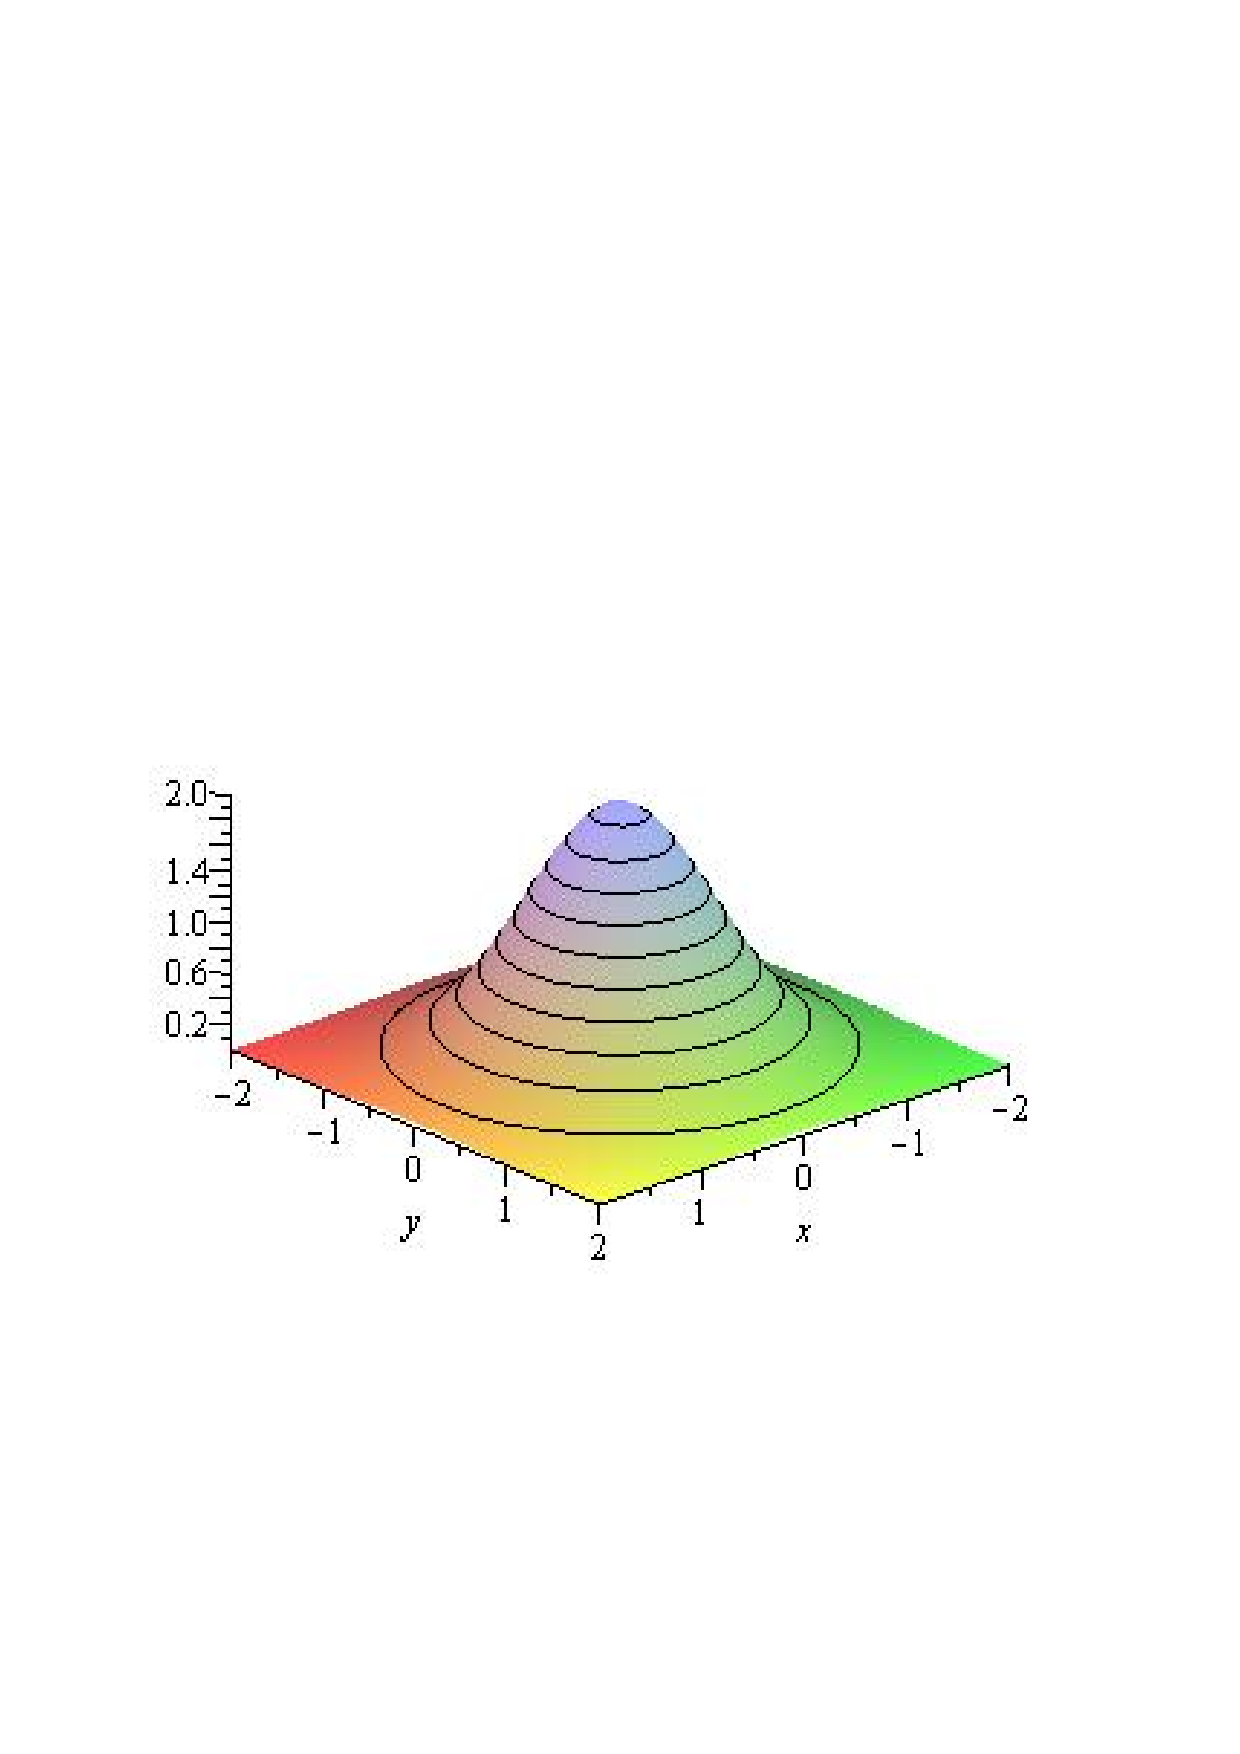
\includegraphics[scale=0.3]{images/max.jpg} & 
 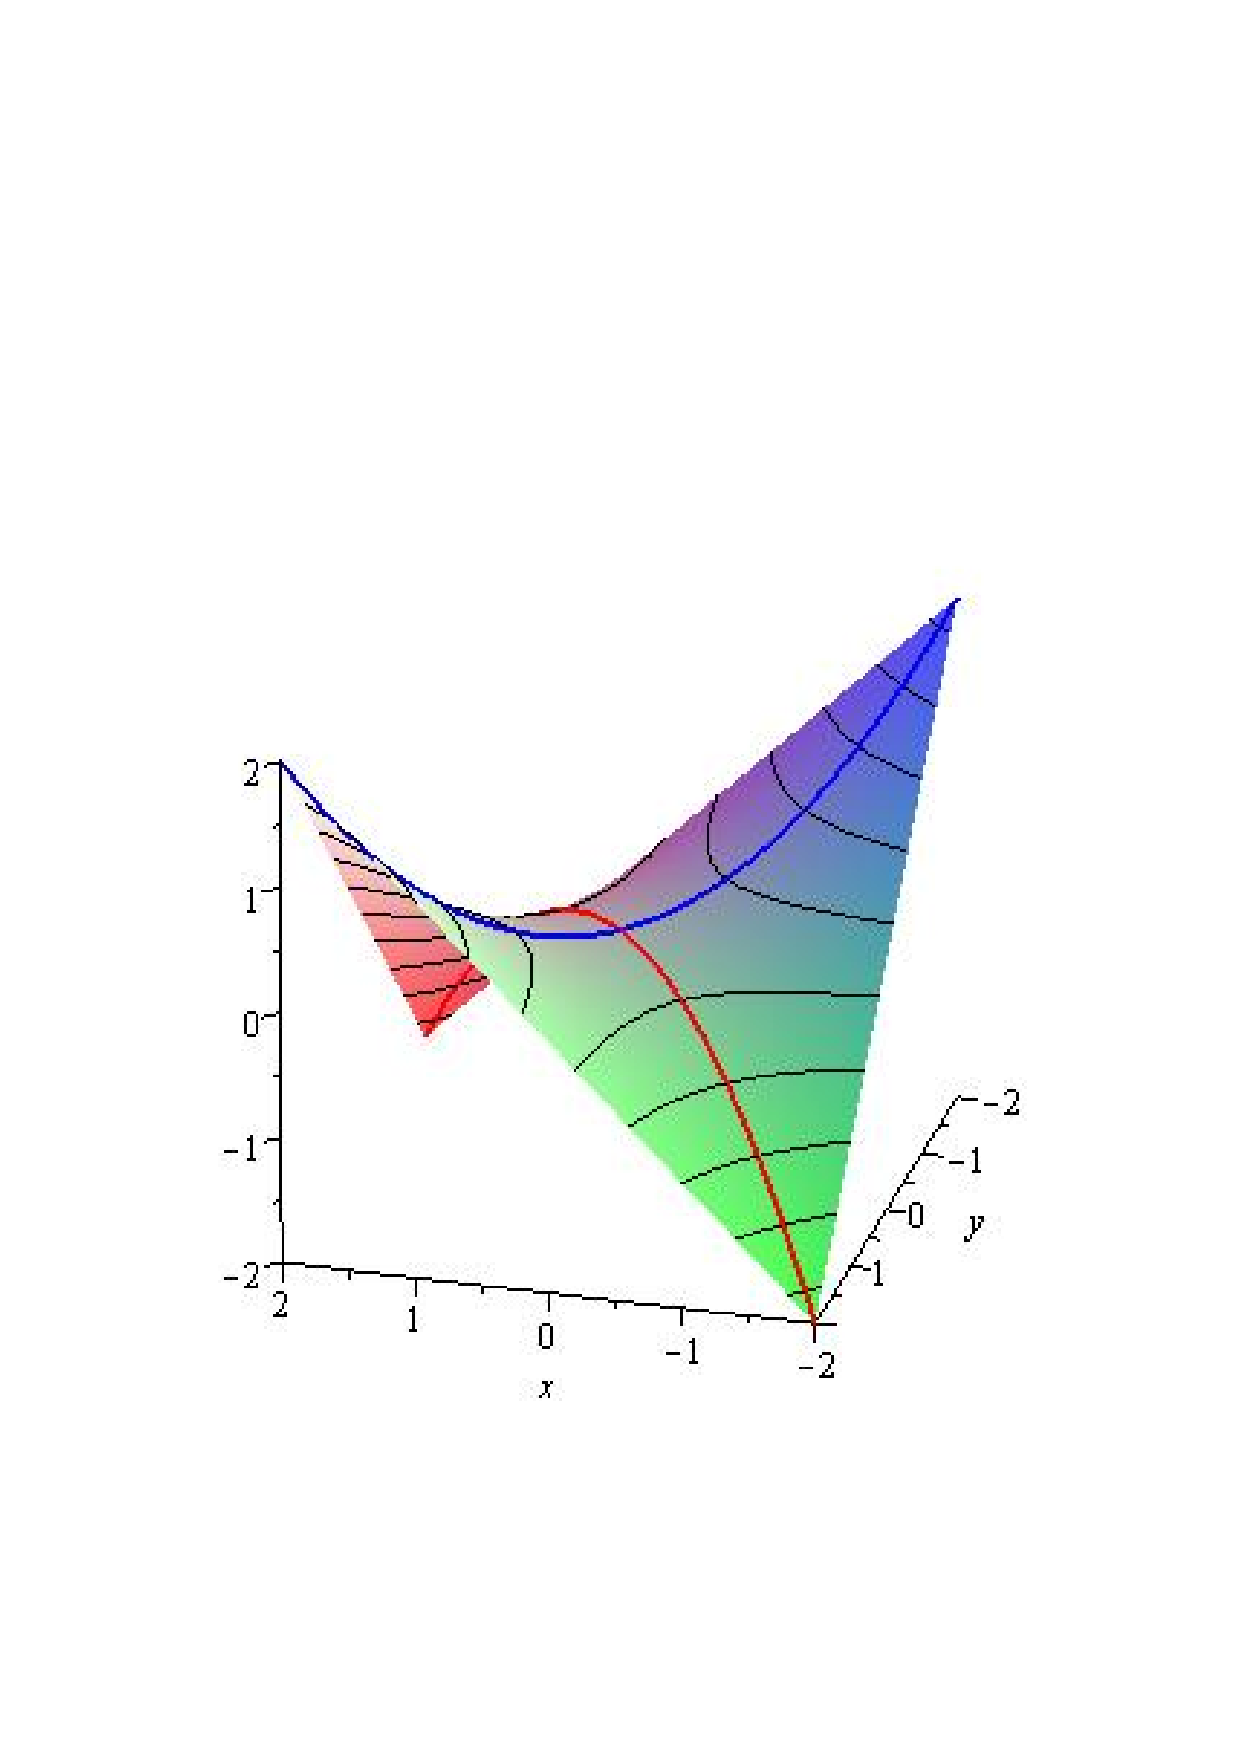
\includegraphics[scale=0.3]{images/saddle.jpg} & 
 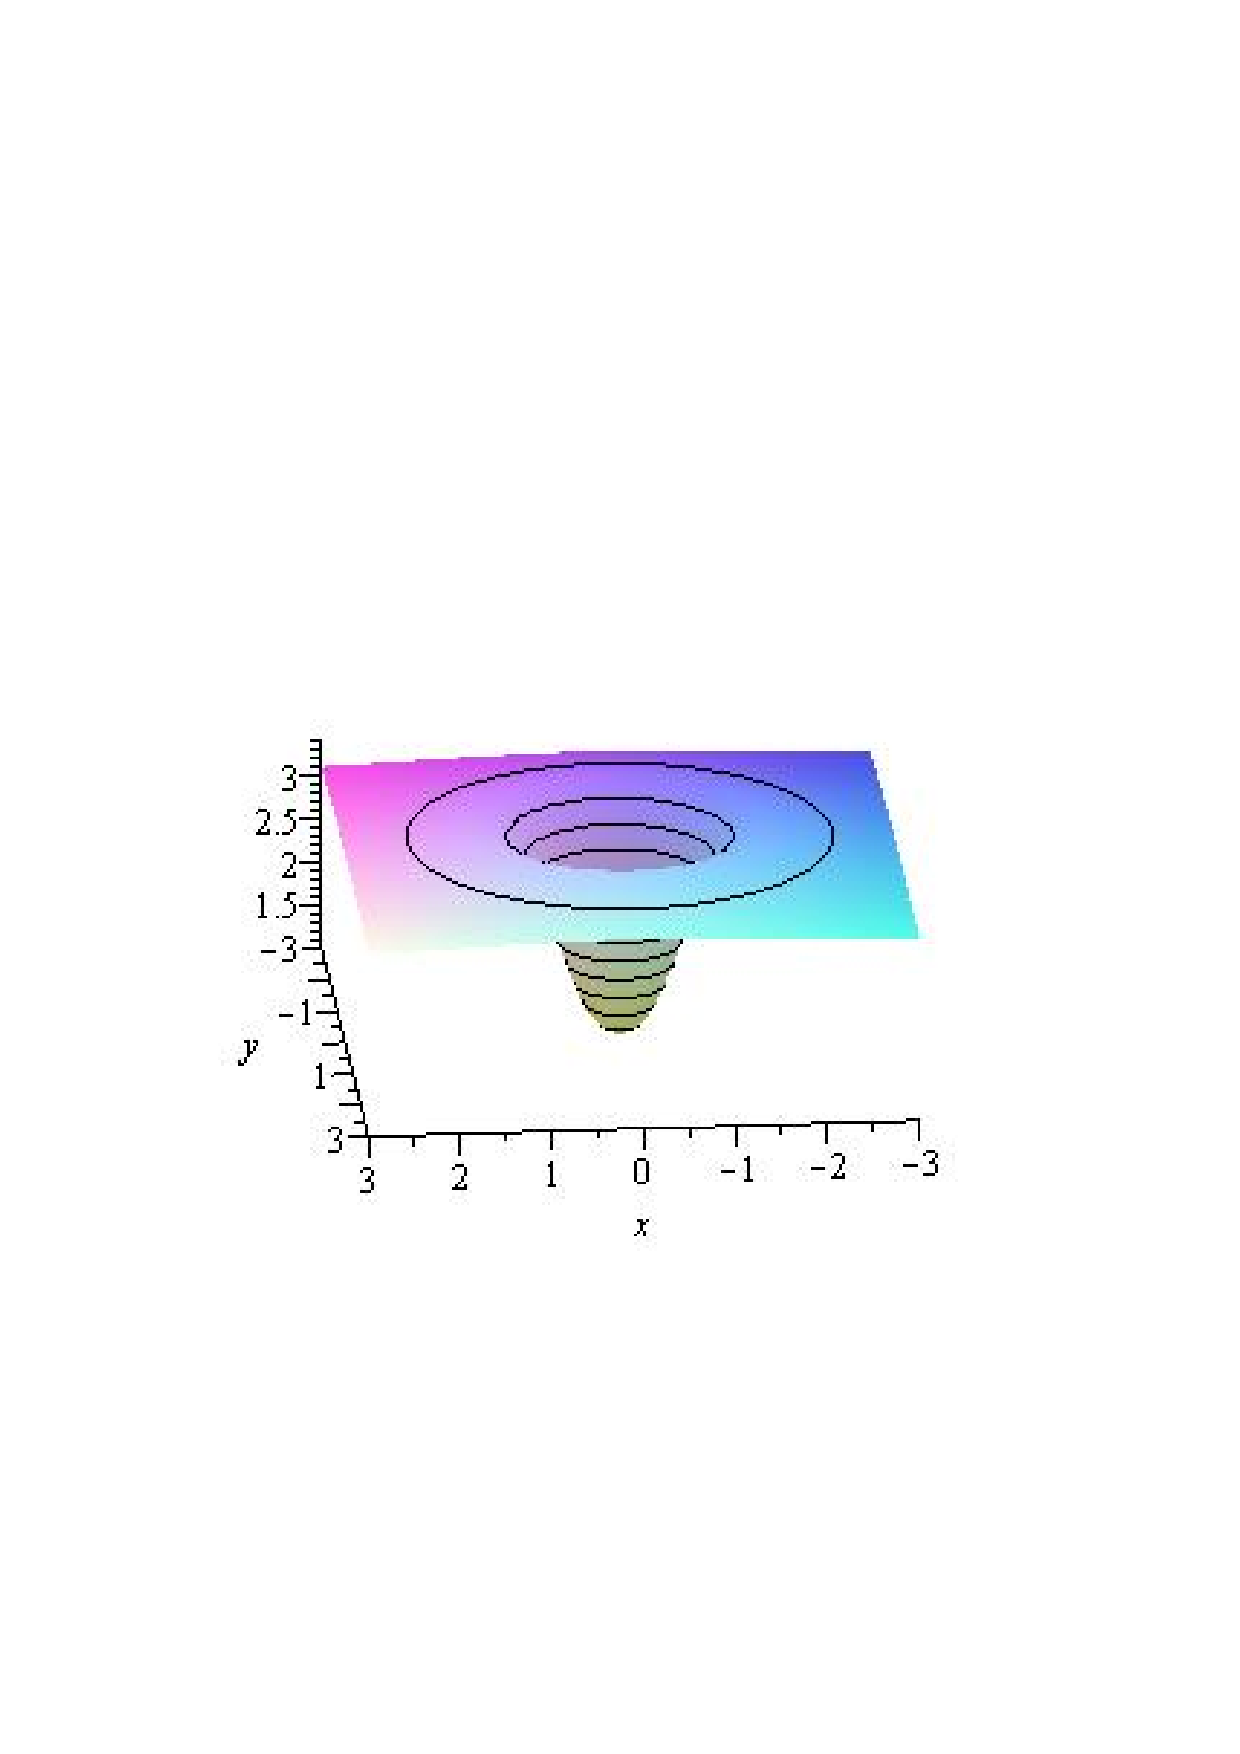
\includegraphics[scale=0.3]{images/min.jpg} \\
 \text{maximum} & \text{saddle point} & \text{minimum}
   \end{array}
\]

At a saddle point we have a local maximum in some directions and a
local minimum in other directions.  

In the one variable case we can classify critical points by looking at
the sign of the second derivative.  In the two variable case, the
analogous criterion involves the Hessian matrix
\[ H = \bbm f_{xx} & f_{xy} \\ f_{xy} & f_{yy} \ebm. \]
The criterion can be stated in terms of the eigenvalues of $H$ or in
terms of the entries of $H$.  The first version is more precise and
more illuminating, but computationally less efficient.  We will state
both versions but we will work mainly with the second one.

\begin{method}\label{meth-hessian-eigenvalues}
 Let $(a,b)$ be a critical point of $f(x,y)$, and let $H$ be the
 Hessian matrix at $(a,b)$.  Let $s$ and $t$ be the eigenvalues of
 $H$.  Then $s$ and $t$ are always real numbers; there is never an
 imaginary part.  Moreover:
 \begin{itemize}
  \item[(a)] If $s,t<0$ then we have a local maximum at $(a,b)$.
  \item[(b)] If $s<0<t$ or $t<0<s$ then we have a saddle point at $(a,b)$.
  \item[(c)] If $0<s,t$ then we have a local minimum at $(a,b)$.
  \item[(d)] If one of $s$ and $t$ is zero, then there are many
   possibilities, and we will not consider them further.  This
   situation rarely occurs in practice.
 \end{itemize}
\end{method}

\begin{method}\label{meth-hessian-entries}
 Alternatively, we can put $A_1=f_{xx}(a,b)$ and 
 \[ A_2 = \det(H)=
     \det\bbm f_{xx}(a,b) & f_{xy}(a,b) \\
              f_{xy}(a,b) & f_{yy}(a,b) \ebm = 
    f_{xx}(a,b) f_{yy}(a,b) - f_{xy}(a,b)^2.
 \]
 \begin{itemize}
  \item[(a)] If $A_1<0$ and $A_2>0$ then we have a local maximum at
   $(a,b)$. 
  \item[(b)] If $A_2<0$ then we have a saddle point at $(a,b)$.
  \item[(c)] If $A_1>0$ and $A_2>0$ then we have a local minimum at
   $(a,b)$. 
  \item[(d)] If $A_2=0$, then there are many possibilities, and we
   will not consider them further.  This situation rarely occurs in
   practice. 
 \end{itemize}
\end{method}

\begin{example}\label{eg-poly-crit-i}
 Consider the function $f(x,y)=x^3+3xy+y^3$.
 The derivatives are
 \begin{align*}
  f_x(x,y)    &= 3x^2+3y & & & f_y(x,y) &= 3x+3y^2 \\
  f_{xx}(x,y) &= 6x & f_{xy}(x,y) &= 3 & f_{yy}(x,y) &= 6y. 
 \end{align*}
 Thus, the critical points are the points $(a,b)$ where $3a^2+3b=0$
 and $3a+3b^2=0$, or equivalently $b=-a^2$ and $a=-b^2$.  Substituting
 the first of these in the second gives $a=-a^4$, so $a^4+a=0$, so
 $(a^3+1)a=0$.  This can only happen if $a=-1$ (in which case
 $b=-a^2=-1$) or $a=0$ (in which case $b=-a^2=0$).  Thus, there are
 two critical points, namely $p=(-1,-1)$ and $q=(0,0)$.  The Hessian
 matrix is $H=\bsm 6x&3\\3&6y \esm$, so $A_1=6x$ and the determinant
 is $A_2=36xy-9=9(4xy-1)$.  At $p$ we have $A_1=-6<0$ and $A_2=27>0$
 so we are in case~(a) of method~\ref{meth-hessian-entries} and we
 have a local maximum.  At $q$ we have $A_1=0$ and $A_2=-9<0$ so we
 are in case~(b) so we have a saddle point.  We can display this
 graphically as follows:
 \[ \includegraphics[scale=0.25]{images/poly_crit_i.jpg} 
     \hspace{5em}
    \includegraphics[scale=0.25]{images/poly_crit_i_contour.jpg} 
 \]
 The picture on the left shows the surface $z=f(x,y)$. The one on the
 right is the corresponding contour plot, which is what you would see
 by looking vertically downwards at the picture on the left.
\end{example}

\begin{example}\label{eg-poly-crit-ii}
 Consider the function 
 \[ f(x,y) = 3x^2+3y^2+2xy(x+y) = 3x^2+3y^2+2x^2y+2xy^2. \]
 The derivatives are 
 \begin{align*}
  f_x(x,y)    &= 6x+4xy+2y^2 & & & f_y(x,y) &= 6y+4xy+2x^2 \\
  f_{xx}(x,y) &= 6+4y & f_{xy}(x,y) &= 4x+4y & f_{yy} &= 6+4x. 
 \end{align*}
 Thus, the critical points are the points $(a,b)$ where
 $6a+4ab+2b^2=0$ and $6b+4ab+2a^2=0$.  If we subtract these two
 equations we get $6a-6b+2b^2-2a^2=0$, which factors as
 $2(a-b)(3-a-b)=0$.  This means that either $a=b$ or $3-a-b=0$.  If
 $a=b$ then our equations become $6a+6a^2=0$, so $a(a+1)=0$, so $a=0$
 or $a=-1$.  We now see that there are critical points at $p_0=(0,0)$
 and $p_1=(-1,-1)$.  Suppose instead that $3-a-b=0$, so $b=3-a$.  In
 this case we have
 \begin{align*}
  0 &= 6a+4ab+2b^2 = 6a+4a(3-a)+2(3-a)^2 \\
    &= 6a+12a-4a^2+2(9-6a+a^2) = -2a^2+6a+18.
 \end{align*}
 By the standard quadratic formula this happens for
 $a=3(1\pm\sqrt{5})/2$, and because $b=3-a$ this gives
 $b=3(1\mp\sqrt{5})/2$.  We therefore have two more critical points:
 \begin{align*}
  p_2 &= (3(1+\sqrt{5})/2,3(1-\sqrt{5})/2) \\
  p_3 &= (3(1-\sqrt{5})/2,3(1+\sqrt{5})/2).
 \end{align*}
\end{example}

\begin{example}\label{eg-sin-crit}
 Consider the function $f(x,y)=\sin(x)\sin(y)$.  The derivatives are 
 \begin{align*}
  f_x(x,y)    &= \cos(x)\sin(y) & & & f_y(x,y) &= \sin(x)\cos(y) \\
  f_{xx}(x,y) &= -\sin(x)\sin(y) & f_{xy}(x,y) &= \cos(x)\cos(y) & f_{yy}(x,y) &= -\sin(x)\sin(y). 
 \end{align*}
 For $f_x$ to be zero, we must have either $\cos(x)=0$ or
 $\sin(y)=0$.  For $f_y$ to be zero, we must have either $\sin(x)=0$
 or $\cos(y)=0$.  At a critical point, both $f_x$ and $f_y$ must be
 zero, so we have one of the following four cases:
 \begin{itemize}
  \item[(p)] $\cos(x)=\sin(x)=0$
  \item[(q)] $\cos(x)=\cos(y)=0$
  \item[(r)] $\sin(y)=\sin(x)=0$
  \item[(s)] $\sin(y)=\cos(y)=0$.
 \end{itemize}
 However, case~(p) cannot actually happen, because
 $\cos(x)^2+\sin(x)^2$ is always equal to one.  Similarly, case~(s)
 cannot happen because $\cos(y)^2+\sin(y)^2$ is always equal to one.

 In case~(r) we have $x=n\pi$ and $y=m\pi$ for some integers $n$ and
 $m$, and $f(x,y)=\sin(n\pi)\sin(m\pi)=0$.  After noting that
 $\cos(k\pi)=(-1)^k$ we see that the Hessian matrix is
 \[ H =
     \bbm -\sin(n\pi)\sin(m\pi) & \cos(n\pi)\cos(m\pi) \\
          \cos(n\pi)\cos(m\pi) & -\sin(n\pi)\sin(m\pi) \ebm = 
     \bbm 0 & (-1)^{n+m} \\ (-1)^{n+m} & 0 \ebm.
 \]
 Thus, in Method~\ref{meth-hessian-entries} we have $A_1=0$ and
 \[ A_2 = 0\tm 0 - (-1)^{n+m}\tm (-1)^{n+m} = -1, \]
 so there is a saddle point at $(n\pi,m\pi)$

 Similarly, in case~(q) we have
 $x=(n+\half)\pi$ and $y=(m+\half)\pi$ for some $n$ and $m$.  From the
 graph of $\sin(x)$ we can observe that $\sin((n+\half)\pi)=(-1)^n$,
 so in these cases we have 
 \[ f(x,y)=\sin((n+\half)\pi)\sin((m+\half)\pi) = (-1)^{n+m}. \]
 The Hessian matrix is
 \[ H =
     \bbm -\sin((n+\half)\pi)\sin((m+\half)\pi) &
          \cos((n+\half)\pi)\cos((m+\half)\pi) \\
          \cos((n+\half)\pi)\cos((m+\half)\pi) &
          -\sin((n+\half)\pi)\sin((m+\half)\pi) \ebm = 
     \bbm (-1)^{n+m+1} & 0 \\ 0 & (-1)^{n+m+1} \ebm.
 \]
 This gives $A_1=(-1)^{n+m+1}$ and 
 \[ A_2 = (-1)^{n+m+1}\tm (-1)^{n+m+1} - 0\tm 0 = 1. \]
 If $n+m$ is even then $A_1=-1<0$ so we have a local maximum (and in
 fact $f=1$).  If $n+m$ is odd then $A_1=1>0$ so we have a local
 minimum (and in fact $f=-1$).  
 \[ \includegraphics[scale=0.5,clip=true,trim=0cm 9cm 0cm 9cm]{images/sinsin_crit.jpg}  \]
\end{example}

\begin{example}\label{eg-gauss-crit}
 Consider the function $f(x,y)=e^{-x^2-y^2-2y}$.  By the chain rule we
 have $f_x(x,y)=-2xe^{-x^2-y^2-2y}$.  The second factor here is
 just $f(x,y)$ again, and it is convenient to write it that way, so
 that $f_x=-2xf$.  For the second derivative we then get 
 \begin{align*}
   f_{xx} &= (-2xf)_x = (-2x)_x\,f + (-2x)\, f_x \\
          &= -2f + (-2x)\,(-2x) f = (4x^2-2)f.
 \end{align*}
 If we write all the other derivatives in terms of $f$ in the same way
 we get
 \begin{align*}
  f_x    &= -2xf & & & f_y &= (-2y-2)f \\
  f_{xx} &= (4x^2-2)f & f_{xy} &= (4xy+4x)f & f_{yy} &= (4y^2+8y+2)f. 
 \end{align*}
 Note that $f$ itself is never zero, so for $f_x=-2xf$ to be zero
 we must have $-2x=0$ or in other words $x=0$.  Similarly, for
 $f_y$ to be zero we must have $(-2y-2)f=0$ and so $y=-1$.  Thus, there is
 only one critical point, namely $p=(0,-1)$.  At this critical point
 we have $-x^2-y^2-2y=-(0)^2-(-1)^2+2=1$ so $f=e^{1}=e$.  The Hessian
 matrix is 
 \[ H = \bbm 4x^2-2 & 4xy+4x \\ 4xy+4x & 4y^2+8y+2 \ebm f =
     \bbm -2e & 0 \\ 0 & -2e \ebm.  
 \]
 In Method~\ref{meth-hessian-entries} we therefore have $A_1=-2e<0$ and
 $A_2=4e^2>0$ so there is a local maximum.
 \[ 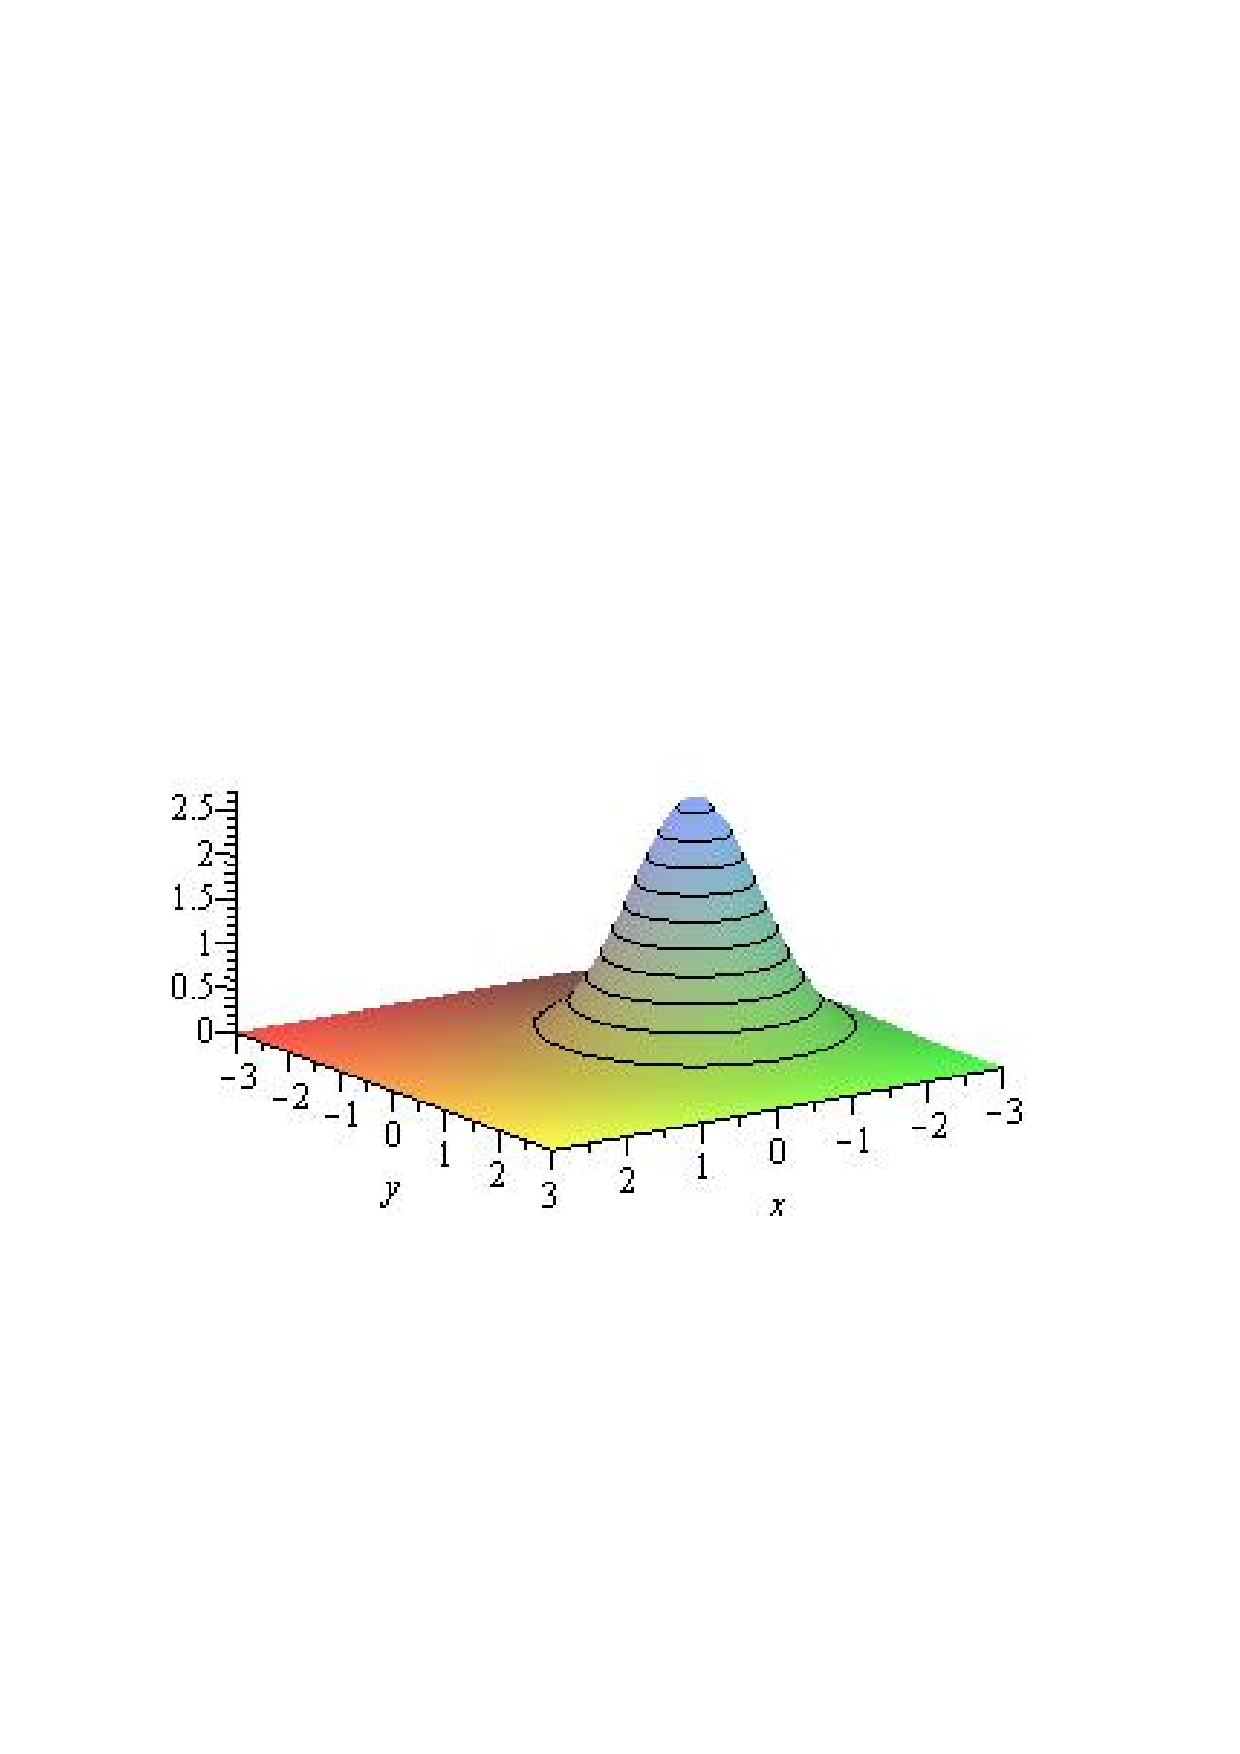
\includegraphics[scale=0.45]{images/gauss_crit.jpg}  \]

\end{example}

\subsection{Functions of three or more variables}
\label{subsec-opt-three}

If $f$ is a function of several variables, then the maximum value of
$f$ (if there is one) will occur at a point where the partial
derivatives with respect to all those variables are zero.  The same
condition will hold for the minimum value.  For example, if $f$ is a
function of $x$, $y$ and $z$, then the maximum and minimum will occur
at a point where $f_x=f_y=f_z=0$.  

It is again possible to classify critical points using the Hessian.
In the three variable case, the Hessian matrix is
\[ H = \bbm f_{xx} & f_{xy} & f_{xz} \\
            f_{yx} & f_{yy} & f_{yz} \\
            f_{zx} & f_{zy} & f_{zz} \ebm 
\]

In terms of eigenvalues, we can say the following:
\begin{method}
 Let $p=(a,b,c)$ be a critical point of $f(x,y,z)$.  Then all the
 eigenvalues of $H$ at $p$ are real.  
 \begin{itemize}
  \item[(a)] If all the eigenvalues are positive, then $f$ has a local
   minimum at $p$. 
  \item[(b)] If all the eigenvalues are negative, then $f$ has a local
   maximum at $p$.
  \item[(c)] If some some eigenvalues are positive and some are
   negative, then we have something like a saddle point.  In
   particular, we definitely do not have a local maximum or local
   minimum.
  \item[(d)] If one or more eigenvalues is zero, then there are
   various possibilities that we will not explore further.
 \end{itemize}
 All this works in the same way if there are more than three
 variables. 
\end{method}

There is also an alternative method involving determinants.
\begin{method}\label{meth-hessian-entries-three}
 Let $p=(a,b,c)$ be a critical point of $f(x,y,z)$.  Put 
 \[ A_1 = f_{xx}
     \hspace{5em}
    A_2 = \det\bbm f_{xx} & f_{xy} \\ f_{yx} & f_{yy} \ebm
     \hspace{5em}
    A_3 = \det\bbm f_{xx} & f_{xy} & f_{xz} \\
                   f_{yx} & f_{yy} & f_{yz} \\
                   f_{zx} & f_{zy} & f_{zz} \ebm, 
 \]
 with everything evaluated at $p$.
 \begin{itemize}
  \item[(a)] If $A_1>0$, $A_2>0$ and $A_3>0$ then $f$ has a local
   minimum at $p$.
  \item[(b)] If $A_1<0$, $A_2>0$ and $A_3<0$ then $f$ has a local
   maximum at $p$. 
  \item[(c)] If $A_1$, $A_2$ and $A_3$ are nonzero but the pattern of
   signs is not as in~(a) or~(b), then we have something like a saddle
   point.  In particular, we definitely do not have a local maximum or
   local minimum.
  \item[(d)] If $A_1=0$ or $A_2=0$ or $A_3=0$, then there are
   various possibilities that we will not explore further.
 \end{itemize}
 All this generalises in a straightforward way if there are more than
 three variables.  We take $A_k$ to be the determinant of the top left
 $k\tm k$ block in the Hessian matrix.  If all the numbers $A_k$ are
 positive we have a local minimum, and if all the numbers $(-1)^kA_k$
 are positive then we have a local maximum.
\end{method}

\begin{example}
 Consider the function $f(x,y,z)=8(x^2+y^2+z^2)-(z+1)^3$.  The first
 derivatives are $f_x=16x$ and $f_y=16y$ and 
 \[ f_z = 16z - 3(z+1)^2 = 
     16z - 3z^2 - 6z + 3 = 
      3+10z-3z^2 = (z-3)(1-3z).
 \]
 This means that the critical points are where $x=y=0$ and
 $(z-3)(3z-1)=0$, so $z=3$ or $z=1/3$.  The Hessian matrix is 
 \[ H = \bbm f_{xx} & f_{xy} & f_{xz} \\
             f_{yx} & f_{yy} & f_{yz} \\
             f_{zx} & f_{zy} & f_{zz} \ebm =
        \bbm 16 & 0  & 0 \\
             0  & 16 & 0 \\
             0  &    & 10-6z \ebm,
 \]
 so 
 \[ A_1 = 16 \hspace{5em} A_2 = 256 \hspace{5em} A_3 = 256(10-6z). \]
 At $(0,0,1/3)$ we get $A_3=1024$ so $A_1$, $A_2$ and $A_3$ are all
 positive, so we have a local minimum.  At $(0,0,3)$ we have
 $A_3=-1024$ so we are in case~(c) of
 Method~\ref{meth-hessian-entries-three} and we have some kind of
 saddle. 
\end{example}

\section{Constrained optimisation}
\label{sec-constrained}

Often we want to find the maximum or minimum value of a function
$f(x,y)$, where $x$ and $y$ cannot vary independently, but are linked
by some kind of constraint, which we can write in the form $g(x,y)=0$
for some other function $g$.

\begin{example}\label{eg-closest}
 We might want to find the closest point to the origin on the line
 with equation $3x+4y=5$.  This amounts to minimising the function
 $f(x,y)=x^2+y^2$ (the squared distance from the origin) subject to
 the constraint $g(x,y)=0$, where $g(x,y)=3x+4y-5$.
\end{example}
\begin{example}\label{eg-tank}
 Suppose we want to make a metal tank of volume $4m^3$.  It will have
 length $x$, width $y$ and height $z$ (measured in metres), and it
 will have a base but no top, so there are five panels altogether, of
 areas $xy$, $xz$, $xz$, $yz$ and $yz$.  The total area of metal sheet
 that we need is thus $f(x,y,z)=xy+2xz+2yz$ (in square metres).  As
 the volume needs to be $4m^3$, the function $g(x,y,z)=xyz-4$ must be
 zero.  To use as little metal as possible, we should minimise $f$
 subject to the constraint $g=0$.
\end{example}

\begin{method}\label{meth-lagrange-mult}
 To maximise $f(x,y,\dotsc)$ subject to the constraint
 $g(x,y,\dotsc)=0$, simply find the unconstrained maximum of the
 function 
 \[ L(\lm,x,y,\dotsc) = f(x,y,\dotsc) - \lm g(x,y,\dotsc) \]
 and ignore the value of $\lm$.  The extra parameter $\lm$ is called a
 \emph{Lagrange multiplier}.
\end{method}

We now explain in outline why this is usually valid.  (If we were more
careful we would discover that certain technical conditions are needed
for the method to work, but we will not explore this in detail here.
The conditions involved are usually satisfied.)  We will focus on the
case where we have just two variables ($x$ and $y$); extra variables
do not change the picture in any essential way.  The solutions of
$g(x,y)=0$ will then form a curve in the plane, called the
\emph{constraint curve}.  Note that
\begin{align*}
 L_\lm(\lm,x,y) &= -g(x,y) \\
 L_x(\lm,x,y) &= f_x(x,y)-\lm g_x(x,y) \\
 L_y(\lm,x,y) &= f_y(x,y)-\lm g_y(x,y).
\end{align*}
At a critical point of $L$, we must therefore have $g(x,y)=0$ (so we
are on the constraint curve) and $f_x=\lm g_x$ and $f_y=\lm g_y$.  Now
suppose we change $x$ and $y$ slightly, by $\dl x$ and $\dl y$ say,
while leaving $\lm$ fixed.  The resulting changes in $f$, $g$ and $h$
will be
\begin{align*}
 \dl f & \simeq \dl x.f_x + \dl y.f_y \\
 \dl g & \simeq \dl x.g_x + \dl y.g_y \\
 \dl h & \simeq \dl x.L_x + \dl y.L_y 
         = \dl x.(f_x-\lm g_x) + \dl y.(f_y-\lm g_y) \\
       &= \dl f - \lm \dl g.
\end{align*}
As $(\lm,x,y)$ is assumed to be a critical point of $h$, we have
$\dl h=0$, or equivalently $\dl h=\lm\,\dl g$.  This works for all
small changes $(\dl x,\dl y)$, including those that move us off the
constraint curve.  We are mostly interested in changes that keep us on
the constraint curve, which means that $g$ remains equal to zero, so
$\dl g=0$.  For such changes the equation $\dl f=\lm\,\dl g$ becomes
$\dl f=0$.  This means that $(x,y)$ is a critical point for the
variation of $f$ along the constraint curve, so it will probably be a
local maximum or minimum.

To understand this in another way, we can imagine a landscape where
the height of the land at position $(x,y)$ is given by $f(x,y)$.  We
can then think of the constraint curve as tracing out a road through
this landscape.  In this context, maximising $f$ subject to
$g=0$ means finding the highest point on the road.  Note that if the
road is crossing the contours, then we can increase $f$ by driving
forwards or backwards a little, so we cannot already have the maximum
possible value of $f$.  Thus, to find the maximum, we need to look for
places where the road is running along the contours, not crossing
them.  The normal vector to the contour through $(a,b)$ is
$\bbm f_x(a,b)\\f_y(a,b)\ebm$, and the normal vector to the road
is $\bbm g_x(a,b)\\ g_y(a,b)\ebm$.  If the road is running along the
contour then these two vectors will be multiples of each other, say
$\bbm f_x\\ f_y\ebm=\lm\bbm g_x\\ g_y\ebm$ at $(a,b)$.  This means
that $L_x(\lm,a,b)=L_y(\lm,a,b)=0$, and as we are on the road we also
have $L_\lm(\lm,a,b)=g(a,b)=0$.  This means that $(\lm,a,b)$ is a
critical point of $L$, as expected.
\[ \includegraphics[clip,trim=2cm 0cm 0cm 4cm,scale=0.3]{images/lg_skirt.jpg}
   \hspace{4em}
   \includegraphics[scale=0.25]{images/lg_contour.jpg}
\]
The image on the left shows the surface $z=f(x,y)$ as a grey mesh.  
The constraint curve where $g(x,y)=0$ is shown in blue in the
$xy$-plane.  The curve on the surface lying directly above it is 
in red.  The problem is to find the highest and lowest points on
the red curve.  The image on the right is what we see when looking 
vertically downwards at the image on the left.  The highest and
lowest points are marked with crosses.  These are where the red 
curve is tangent to the contours.

\begin{example}\label{eg-closest-again}
 In Example~\ref{eg-closest}, we wanted to minimise $f(x,y)=x^2+y^2$
 subject to the constraint $g(x,y)=3x+4y-5=0$.  To do this, we need to
 find the unconstrained minimum of the function 
 \[ L(\lm,x,y) = x^2+y^2-\lm(3x+4y-5). \]
 The critical points are the places where the following partial
 derivatives are zero:
 \begin{align*}
  L_\lm(\lm,x,y) &= -g(x,y) = -3x-4y+5 \\
  L_x(\lm,x,y) &= 2x-3\lm \\
  L_y(\lm,x,y) &= 2y-4\lm.
 \end{align*}
 The equations $2x-3\lm=2y-4\lm=0$ give $x=3\lm/2$ and $y=2\lm$.
 Substituting these into the equation $3x+4y-5=0$ gives
 $9\lm/2+8\lm=5$, which simplifies to $\lm=2/5$.  Substituting this
 back into $x=3\lm/2$ and $y=2\lm$ gives $(x,y)=(3/5,4/5)$.  At this
 point we have $f(x,y)=(3/5)^2+(4/5)^2=(9+16)/25=1$.  We conclude that
 the minimum value of $f$ is $1$, and that this occurs at the point
 $(3/5,4/5)$. 
 \begin{center}
  \begin{tikzpicture}[scale=2]
   \draw[->] (-2,0) -- (2,0);
   \draw[->] (0,-2) -- (0,2);
   \draw[dotted,blue] (0,0) circle(0.2);
   \draw[dotted,blue] (0,0) circle(0.4);
   \draw[dotted,blue] (0,0) circle(0.6);
   \draw[dotted,blue] (0,0) circle(0.8);
   \draw[dotted,blue] (0,0) circle(1.2);
   \draw[dotted,blue] (0,0) circle(1.4);
   \draw[dotted,blue] (0,0) circle(1.6);
   \fill[white] (0.5,0.7) rectangle (2,0.9); 
   \draw[red] (-1,2) -- (2,-0.25);
   \draw[       blue] (0,0) circle(1.0);
   \fill (0.6,0.8) circle(0.03);
   \draw(0.7,0.8) node[anchor=west] {$(3/5,4/5)$};
   \draw(2,-0.25) node[anchor=north west] {$3x+4y-5=0$};
  \end{tikzpicture}
 \end{center}
\end{example}

\begin{example}\label{eg-tank-again}
 In Example~\ref{eg-tank} we wanted to minimise $f(x,y,z)=xy+2xz+2yz$
 subject to the constraint $g(x,y,z)=xyz-4=0$.  To do this, we need to
 find the unconstrained minimum of the function 
 \[ L(\lm,x,y,z) = xy+2xz+2yz - \lm(xyz-4). \]
 The critical points are the places where the following partial
 derivatives are zero:
 \begin{align*}
  L_\lm(\lm,x,y,z) &= -g(x,y,z) = 4-xyz \\
  L_x(\lm,x,y,z)   &= y+2z-\lm y z \\
  L_y(\lm,x,y,z)   &= x+2z-\lm x z \\
  L_z(\lm,x,y,z)   &= 2x+2y-\lm x y.
 \end{align*}
 We can rearrange these equations as follows:
 \begin{align*}
  xyz &= 4 \tag{A} \\
   z^{-1}+2y^{-1} &= \lm  \tag{B} \\
   z^{-1}+2x^{-1} &= \lm  \tag{C} \\
  2y^{-1}+2x^{-1} &= \lm. \tag{D}
 \end{align*}
 By subtracting equations~(B) and~(C) we see that $y^{-1}=x^{-1}$, so
 $x=y$.  After substituting this in~(D) we get $4x^{-1}=4y^{-1}=\lm$,
 so $x=y=4/\lm$.  We can then substitute this in~(C) to get
 $z^{-1}+\lm/2=\lm$, so $z=2/\lm$.  Now~(A) becomes
 $(4/\lm)(4/\lm)(2/\lm)=4$, so $32=4\lm^3$, so $\lm=(32/4)^{1/3}=2$.
 This gives $x=4/\lm=2$, and similarly $y=2$ and $z=1$.  For these
 values of $x$, $y$ and $z$ we have $f(x,y,z)=f(2,2,1)=12$.  Thus, the
 most efficient design is to make the dimensions of the tank
 $2\tm 2\tm 1$ metres, and we then need $12m^2$ of metal sheet.

 (Note, incidentally, that in our initial rearrangement we divided the
 equation $y+2z-\lm yz=0$ by $yz$ to get $z^{-1}+2y^{-1}=\lm$.  This
 would not be valid if $yz$ were zero.  Fortunately, $yz$ cannot be
 zero, because we have $xyz=4$.  You should be careful to check this
 kind of thing when dividing.)
\end{example}

\begin{example}
 Suppose we want to maximise $f(x,y)=x+y$ subject to the constraint
 $x^2/a+y^2/b=1$ (for some constants $a,b>0$).  Here we must take
 $g(x,y)=x^2/a+y^2/b-1$ and so
 \[ L(\lm,x,y) = x+y-\lm(x^2/a+y^2/b-1). \]
 The critical points are the places where the following partial
 derivatives are zero:
 \begin{align*}
  L_\lm(\lm,x,y) &= g(x,y) = x^2/a+y^2/b-1 \\
  L_x(\lm,x,y) &= 1-2x\lm/a \\
  L_y(\lm,x,y) &= 1-2y\lm/b.
 \end{align*}
 The equations $1-2x\lm/a=1-2y\lm/b=0$ give $x=a/(2\lm)$ and
 $y=b/(2\lm)$.  We can substitute these values in the equation
 $x^2/a+y^2/b=1$ to get $a/(4\lm^2)+b/(4\lm^2)=1$, which can be
 rearranged as $\lm^2=(a+b)/4$, so
 $\lm=\pm\sqrt{a+b}/2$.  As $x=a/(2\lm)$ and $y=b/(2\lm)$ we get 
 \[ (x,y) =
     \pm \left(\frac{a}{\sqrt{a+b}},\frac{b}{\sqrt{a+b}}\right).
 \]
 For these points we have 
 \[ f(x,y)=x+y=\pm(a+b)/\sqrt{a+b} = \pm\sqrt{a+b}. \]
 This means that the maximum possible value of $f$ (subject to the
 constraint) is $\sqrt{a+b}$, and the minimum is $-\sqrt{a+b}$.

 This can be illustrated as follows:
 \begin{center}
  \begin{tikzpicture}[scale=2]
   \draw[->] (-1.5,0) -- (1.5,0);
   \draw[->] (0,-1.5) -- (0,1.6);
   \foreach \t in {0,0.2,...,3} {
    \draw[blue,dotted] ({\t-1.5},1.5) -- (1.5,{\t-1.5});
    \draw[blue,dotted] ({1.5-\t},-1.5) -- (-1.5,{1.5-\t});
   }
   \fill[white] (0.8,-0.6) rectangle (1.5,-0.9);
   \fill[white] (0.5,1) rectangle (1.5,1.3);
   \draw[blue] ( 0.1, 1.5) -- ( 1.7,-0.1);
   \draw[blue] (-0.1,-1.5) -- (-1.7, 0.1);
   \draw[red,domain=0:360,samples=300,smooth,variable=\t]
    plot({0.96*cos(\t)},{1.28*sin(\t)});
   \fill ( 0.576, 1.024) circle(0.03);
   \fill (-0.576,-1.024) circle(0.03);
   \draw (0.9,-0.75) node[anchor=west]{$g(x,y)=0$};
   \draw ( 1.7,-0.1) node[anchor=west]{$f(x,y)=\sqrt{a+b}$};
   \draw (-1.7, 0.1) node[anchor=east]{$f(x,y)=-\sqrt{a+b}$};
   \draw ( 0.6,1.15) node[anchor=west]{$(a/\sqrt{a+b},b/\sqrt{a+b})$};
  \end{tikzpicture}
 \end{center}
\end{example}

We now consider the problem of optimisation when there are several
constraints. 
\begin{method}\label{meth-lagrange-multi}
 To find the maximum and minimum values of $f(x,y,\dotsc)$ subject to
 two constraints $g=0$ and $h=0$, we find the unconstrained critical
 points of the function 
 \[ L(\lm,\mu,x,y,\dotsc) =
     f(x,y,\dotsc) - \lm g(x,y,\dotsc) - \mu h(x,y,\dotsc)
 \]
 (and then ignore the values of $\lm$ and $\mu$).  More generally, if
 there are constraints $g_1=0,\dotsc,g_r=0$ then we use
 \[ L(\lm_1,\dots,\lm_r,x,y,\dotsc) =
      f(x,y,\dotsc) - \sum_{i=1}^r \lm_i g_i(x,y,\dotsc).
 \]
\end{method}

\begin{example}\label{eg-two-constraints}
 Suppose we want to maximise $z$ subject to the constraints
 $x^2+y^2+z^2=9$ and $x+2y+4z=3$.  For this we need the unconstrained
 critical points of the function 
 \[ L = z - \lm(x^2+y^2+z^2-9) - \mu(x+2y+4z-3). \]
 The partial derivatives $L_\lm$, $L_\mu$, $L_x$, $L_y$ and $L_z$ must
 all be zero, which gives the following equations:
 \begin{align*}
  x^2+y^2+z^2      &= 9  \tag{A} \\
  x+2y+4z          &= 3  \tag{B} \\
    -2\lm x -  \mu &= 0  \tag{C} \\
    -2\lm y - 2\mu &= 0  \tag{D} \\
  1 -2\lm z - 4\mu &= 0. \tag{E}
 \end{align*}
 These equations are sufficiently complex that in practice you would
 probably use a computer to solve them.  Nonetheless, it is possible
 to explain the solution by hand, as follows.  We first multiply
 equation~(C) by $x$, and equation~(D) by $y$, and equation~(E) by
 $z$, and add them together to get
 \[ z -2\lm(x^2+y^2+z^2) - \mu(x+2y+4z) = 0. \]
 We can now substitute equations~(A) and~(B) in this to get
 \[ z - 18\lm - 3\mu = 0. \tag{F} \]
 Alternatively, we can add equation~(C) to $2$ times equation~(D) and
 $4$ times equation~(E) to get
 \[ 4 - 2\lm(x+2y+4z) - 21\mu = 0. \]
 We can now substitute equation~(B) in this to get $4-6\lm-21\mu=0$,
 so 
 \[ \lm = \tfrac{7}{2}\mu - \tfrac{2}{3}. \tag{G} \]
 Subtracting $3$ times~(G) from~(F) gives 
 \[ z = 12-60\mu. \tag{H} \]
 If we substitute~(G) and~(H) in~(E) and expand out, we get
 $-15+160\mu-420\mu^2=0$.  Solving this quadratic equation in the
 usual way, we get $\mu=1/6$ or $\mu=3/14$.  If $\mu=1/6$ then~(G)
 and~(H) become $\lm=1/12$ and $z=2$.  After substituting these values
 into~(C) and~(D) we get $x=-1$ and $y=-2$.  Thus, we have a critical
 point of $L$ at 
 \[ (\lm,\mu,x,y,z) = (1/12,1/6,-1,-2,2). \]
 On the other hand, if $\mu=3/14$ then~(G) and~(H) become $\lm=-1/12$
 and $z=-6/7$.  After substituting these into~(C) and~(D) we get
 $x=9/7$ and $y=18/7$.  Thus, we have a critical
 point of $L$ at 
 \[ (\lm,\mu,x,y,z) = (-1/12,3/14,9/7,18/7,-6/7). \]
 Thus, the maximum value of $z$ is $2$ (at the first critical point)
 and the minimum is $-6/7$ (at the second critical point).

 Geometrically, the constraint $x^2+y^2+z^2=9$ corresponds to a sphere
 of radius three around the origin, and the constraint $x+2y+4z=3$
 corresponds to a plane that cuts through the sphere.  We are
 interested in points $(x,y,z)$ where both constraints hold.  These
 lie on the intersection of the sphere with the plane, which is the
 sloping circle in the picture on the left below.  The picture on the
 right shows the same circle together with the planes $z=-6/7$ and
 $z=2$, showing that these are indeed the maximum and minimum values
 of $z$ on the curve.
 \[
  \includegraphics[clip=true,trim=4cm 4cm 4cm 4cm,scale=0.35]{images/cut_sphere.jpg}
  \includegraphics[clip=true,trim=4cm 4cm 4cm 4cm,scale=0.35]{images/cut_sphere_levels.jpg}
 \]
\end{example}

\section{Multiple integrals}

\subsection{Integrals over plane regions}
\label{subsec-plane-integrals}

Let $D$ be a region in the plane, and let $f(x,y)$ be a function
defined for points $(x,y)$ in $D$.  We define the integral 
$\iint_D f(x,y)dA$ as follows.  First, we divide the region $D$
into a large number of small regions $D_1,\dotsc,D_n$.  As each region
$D_i$ is small, the value of $f$ will not change much as we move
around $D_i$, so it makes approximate sense to talk about the value of
$f$ on $D_i$ as a single number.  The integral is approximately
defined by 
\[ \iint_D f(x,y)\,dA = \sum_{i=1}^N 
    (\text{ value of $f$ on $D_i$ }) \times (\text{ area of } D_i).
\]
To get the exact value, we divide $D$ into a larger and larger number
of smaller and smaller pieces, and then pass to the limit.  It takes
considerable work to formulate this in a precise and rigorous way, but
this general idea will be sufficient for our purposes.

Some applications of this kind of integration are as follows.
\begin{itemize}
 \item[(a)] Suppose that the region $D$ is a charged plate, and that
  the charge density at a point $(x,y)$ is $q(x,y)$; then the total
  charge is $Q=\iint_Dq(x,y)\,dA$.
 \item[(b)] Suppose that the region $D$ represents a structure of
  constant density $\rho$ and vertical thickness $f(x,y)$ attached to
  an axle passing vertically through the origin.  Then the mass of the
  structure is $\iint_D\rho f(x,y)\,dA$, whereas the moment of
  inertia (which measures the difficulty of turning the axle) is
  $\iint_D\rho f(x,y)(x^2+y^2)dA$.
 \item[(c)] Suppose that the region $D$ represents a large solar cell,
  with the brightness of light arriving at $(x,y)$ being given by the
  function $f(x,y)$.  Then the total incident power on the cell will
  be (a constant times) $\iint_Df(x,y)\,dA$.  
 \item[(d)] The total area of a region $D$ is just $\iint_D 1\,dA$.
 \item[(e)] Suppose we have a solid region $E$ in three-dimensional
  space.  Often $E$ can be described as follows: there is a
  two-dimensional region $D$ that is the shadow of $E$ in the
  $(x,y)$-plane, and the vertical line through $(x,y)$ meets $E$ at
  height $f(x,y)$ and leaves it at height $g(x,y)$ say.  The total
  volume of $E$ is then $\iint_D g(x,y)-f(x,y)\,dA$.
\end{itemize}

In the simplest case, the region $D$ is a rectangle aligned with the
axes, given by $a\leq x\leq b$ and $c\leq y\leq d$ say.  In this case
we can just divide the horizontal interval $[a,b]$ into small
intervals of length $\dl x$, and divide the vertical interval $[c,d]$
into small intervals of length $\dl y$.  This divides $D$ into small
rectangles of area $\dl A=\dl x.\dl y$.  

\renewcommand{\ss}      {\scriptstyle}

\begin{center}
 \begin{tikzpicture}[scale=3]
  \draw[->] (-0.1,0) -- (3.1,0);
  \draw[->] (0,-0.1) -- (0,2.1);
  \fill[green!20] (0.7,0.4) rectangle(2.8,1.6);
  \draw[gray] (0.7,0) -- (0.7,1.6);
  \draw[gray] (2.8,0) -- (2.8,1.6);
  \draw[gray] (0,0.4) -- (2.8,0.4);
  \draw[gray] (0,1.6) -- (2.8,1.6);
  \fill[black] (0.7,0) circle(0.02);
  \fill[black] (2.8,0) circle(0.02);
  \fill[black] (0,0.4) circle(0.02);
  \fill[black] (0,1.6) circle(0.02);
  \draw (0.7,-0.15) node{$a$};
  \draw (2.8,-0.15) node{$b$};
  \draw (-0.15,0.4) node{$c$};
  \draw (-0.15,1.6) node{$d$};
  \filldraw[fill=blue!40,draw=black] (1.5,1) rectangle(1.7,1.15);
  \draw (1.60,0.94) node{$\ss \dl x$};
  \draw (1.77,1.07) node{$\ss \dl y$};
 \end{tikzpicture}
\end{center}
Using this kind of subdivision, we see that the area integral is just
obtained by integrating with respect to both variables $x$ and $y$:
\[ \iint_D f(x,y)\,dA =
    \int_{x=a}^b \left(\int_{y=c}^d f(x,y)\,dy\right)\,dx.
\]

\begin{example}\label{eg-rectangle}
 Let $D$ be the rectangle where $0\leq x\leq 2$ and $0\leq y\leq 3$.
 Then 
 \[ \iint_D x^3+y^2\,dA =
     \int_{x=0}^2 \left(\int_{y=0}^3 x^3+y^2 \,dy\right) dx
 \]
 In the inner integral, we treat $x$ as a constant and $y$ as a
 variable.  This gives
 \[ \int_{y=0}^3 x^3+y^2\,dy =
     \CH{x^3y + y^3/3}_{y=0}^3 =
      (3x^3+27/3)-(0) = 3x^3+9.
 \] 
 The meaning of this intermediate result is as follows: if we take a
 thin strip running horizontally from $x$ to $x+\dl x$, and vertically
 all the way from $0$ to $3$, then the sum of the corresponding
 contributions is approximately $(3x^3+9)\dl x$ (and the approximation
 becomes exact in the limit as $\dl x\to 0$).  
 \begin{center}
  \begin{tikzpicture}[scale=2]
   \filldraw[draw=gray,fill=green!20] (0,0) rectangle(2,3);
   \draw[->] (-0.1,0) -- (2.1,0);
   \draw[->] (0,-0.1) -- (0,3.1);
   \fill[black] (0,0) circle(0.03);
   \fill[black] (2,0) circle(0.03);
   \fill[black] (0,3) circle(0.03);
   \draw (2,-0.15) node{$2$};
   \draw (-0.15,3) node{$3$};
   \filldraw[fill=blue!40,draw=black] (0.5,0) rectangle(0.7,3);
   \fill[black] (0.5,0) circle(0.02);
   \fill[black] (0.7,0) circle(0.02);
   \draw (0.45,-0.08) node{$\ss x$};
   \draw (0.85,-0.08) node{$\ss x+\dl x$};
  \end{tikzpicture}
 \end{center}
 We can now perform the outer integral to add up the contributions
 from all such vertical strips.
 \[ \int_{x=0}^2 3x^3 + 9 \, dx = 
     \CH{3x^4/4 + 9x}_{x=0}^2 = 
      (12 + 18) - (0) = 30.
 \]
 The conclusion is that $\iint_D x^3+y^2\,dA=30$.
\end{example}
\begin{example}
 Let $D$ be the square where $0\leq x\leq\pi$ and
 $-\pi/2\leq y\leq\pi/2$.  Then  
 \[ \iint_D \sin(x)\cos(y)\,dA = 
     \int_{x=0}^\pi\left(
      \int_{y=-\pi/2}^{\pi/2} \sin(x)\cos(y)\,dy
       \right) dx.
 \]
 In the inner integral, we treat $x$ as a constant and $y$ as a
 variable.  This gives
 \[ \int_{y=-\pi/2}^{\pi/2} \sin(x)\cos(y)\,dy = 
     \sin(x) \CH{\sin(y)}_{y=-\pi/2}^{\pi/2} =
      \sin(x)(1-(-1)) = 2\sin(x). 
 \]
 Again, this means that the contribution coming from a vertical strip
 of width $\dl x$ is approximately $2\sin(x)\dl x$.  We can now
 perform the outer integral to add up the contributions from all such
 vertical strips:
 \[ \int_{x=0}^{\pi} 2\sin(x)\,dx = 
     2\CH{-\cos(x)}_0^{\pi} = 
      2(1-(-1)) = 4.
 \]
 The conclusion is that $\iint_D \sin(x)\cos(y)\,dA=4$.  
\end{example}

Note that in both the last two examples, the final answer is just a
number, not a function of $x$ or $y$.  This is as it should be: we
have added up all the contributions from all the different values of
$x$ and $y$, so there is no dependence on $x$ and $y$ left at the
end.  There are various common errors that lead to final answers
depending on $x$ and $y$.  If you end up with such an answer, you
should immediately realise that something has gone wrong.

We now consider Example~\ref{eg-rectangle} again.  We previously did
this by dividing the rectangle $D$ into thin vertical strips,
performing an inner integral over $y$ to calculate the contribution
from each strip, and then integrating over $x$ to add up these
contributions.  We could equally well divide the rectangle into thin
horizontal strips instead.  We would then need to perform an inner
integral over $x$ to find the contribution from each horizontal strip,
and then an outer integral over $y$ to add up these contributions.  In
symbols, we have 
\[ \iint_D x^3+y^2\,dA = 
    \int_{y=0}^3 \left(\int_{x=0}^2 x^3+y^2\,dx\right) dy.
\]
In the inner integral, we treat $y$ as a constant and $x$ as a
variable.  This gives 
\[ \int_{x=0}^2 x^3+y^2\,dx = 
    \CH{ x^4/4 + xy^2 }_{x=0}^2 = 
     (16/4+2y^2)-(0) = 4 + 2y^2,
\]
meaning that the contribution from a horizontal strip of width $\dl y$
at height $y$ is approximately $(4+2y^2)\dl y$.  We can now perform
the outer integral to add up the contributions from all such
horizontal strips:
\[ \int_{y=0}^3 4+2y^2\,dy = \CH{4y+2y^3/3}_{y=0}^3 =
    (12+2\tm 27/3)-(0) = 30.
\]
As expected, this gives the same answer $\iint_D x^3+y^2\,dA=30$ as
before. 

The next simplest type of region that we want to consider is a
triangle.  
\begin{example}\label{eg-triangle-vertical}
 Let $D$ be the triangular region with vertices at $(0,0)$, $(1,0)$
 and $(1,1)$.  
 \begin{center}
  \begin{tikzpicture}[scale=4]
   \fill[green!20] (0,0) -- (1,0) -- (1,1) -- (0,0);
   \draw[->] (0,0) -- (1.1,0);
   \draw[->] (0,0) -- (0,1.1);
   \draw (0,0) -- (1,1) -- (1,0);
   \fill[black] (0,0) circle(0.015);
   \fill[black] (1,0) circle(0.015);
   \fill[black] (1,1) circle(0.015);
   \draw (0,-0.1) node{$(0,0)$};
   \draw (1,-0.1) node{$(1,0)$};
   \draw (1, 1.1) node{$(1,1)$};
   \draw (0.4, 0.6) node {$y=x$};
   \draw (0.5,-0.1) node {$y=0$};
   \draw (1.2, 0.5) node {$x=1$};
  \end{tikzpicture}
 \end{center}
 We will calculate $\iint_D e^{2x-2y}\,dA$.  One approach is to
 divide the region into thin vertical strips: 
 \begin{center}
  \begin{tikzpicture}[scale=4]
   \filldraw[draw=gray,fill=green!20] (0,0) -- (1,0) -- (1,1) -- (0,0);
   \draw[->] (0,0) -- (1.1,0);
   \draw[->] (0,0) -- (0,1.1);
   \draw (0,0) -- (1.1,1.1);
   \fill[black] (0,0) circle(0.015);
   \fill[black] (1,0) circle(0.015);
   \fill[black] (1,1) circle(0.015);
   \draw (0,-0.1) node{$(0,0)$};
   \draw (1,-0.1) node{$(1,0)$};
   \draw (0.9,1.05) node{$(1,1)$};
   \draw (1.25,1.1) node {$y=x$};
   \filldraw[fill=blue!40,draw=black] (0.6,0) -- (0.65,0) -- (0.65,0.65) -- (0.6,0.6) -- (0.6,0);
   \fill[black] (0.60,0) circle(0.013);
   \fill[black] (0.65,0) circle(0.013);
   \draw (0.55,-0.08) node{$\ss x$};
   \draw (0.75,-0.08) node{$\ss x+\dl x$};
  \end{tikzpicture}
 \end{center}
 The strip shown runs from $y=0$ to $y=x$, so the contribution from
 that strip is 
 \[ \dl x . \int_{y=0}^x e^{2x-2y}\,dy =
     \dl x \CH{e^{2x-2y}/(-2)}_{y=0}^x =
      \dl x (e^0-e^{2x})/(-2) = \half (e^{2x}-1) \dl x.
 \]
 To add up the contributions for all such strips, we need to integrate
 over all values of $x$ that occur in $D$, which means from $x=0$ to
 $x=1$.  This gives
 \[ \iint_D e^{2x-2y}\,dA = 
     \int_{x=0}^1 \half (e^{2x}-1)\,dx =
      \CH{\half(\half e^{2x}-x)}_{x=0}^1 = 
       \half(\half e^2-1) - \half(\half-0) = (e^2-3)/4.
 \]
\end{example}

\begin{example}\label{eg-triangle-horizontal}
 As an alternative, we could divide the triangle into horizontal
 strips:
 \begin{center}
  \begin{tikzpicture}[scale=4]
   \filldraw[draw=gray,fill=green!20] (0,0) -- (1,0) -- (1,1) -- (0,0);
   \draw[->] (0,0) -- (1.1,0);
   \draw[->] (0,0) -- (0,1.1);
   \draw (0,0) -- (1.1,1.1);
   \fill[black] (0,0) circle(0.015);
   \fill[black] (1,0) circle(0.015);
   \fill[black] (1,1) circle(0.015);
   \draw (0,-0.1) node{$(0,0)$};
   \draw (1,-0.1) node{$(1,0)$};
   \draw (0.9,1.05) node{$(1,1)$};
   \draw (1.25,1.1) node {$y=x$};
   \draw[dotted] (0,0.40) -- (0.40,0.40);
   \draw[dotted] (0,0.45) -- (0.45,0.45);
   \filldraw[fill=blue!40,draw=black]
    (0.4,0.4) -- (1,0.4) -- (1,0.45) -- (0.45,0.45) -- (0.4,0.4);
   \fill[black] (0,0.40) circle(0.013);
   \fill[black] (0,0.45) circle(0.013);
   \draw (-0.04,0.37) node[anchor=east]{$\ss y$};
   \draw (-0.04,0.46) node[anchor=east]{$\ss y+\dl y$};
  \end{tikzpicture}
 \end{center}
 The left hand end of the strip is at $x=y$, and the right hand end is
 at $x=1$.  Thus, the contribution from the strip is 
 \[ \dl y . \int_{x=y}^1 e^{2x-2y} dx =
     \dl y . \CH{ \half e^{2x-2y} }_{x=y}^1 = 
      \dl y . (\half e^{2-2y} - \half).
 \]
 To add up the contributions for all such strips, we need to integrate
 over all values of $y$ that occur in $D$, which means from $y=0$ to
 $y=1$.  This gives
 \[ \iint_D e^{2x-2y}\,dA = 
     \int_{y=0}^1 \half (e^{2-2y}-1)\,dy =
      \CH{\half(-\half e^{2-2y}-y)}_{y=0}^1 = 
       \half(-\half-1) - \half(-\half e^2-0) = (e^2-3)/4,
 \]
 just as before.
\end{example}

\begin{example}
 Suppose we have a metal sheet $D$ in the shape of a triangular wedge,
 with one vertex at the origin and the other two at $(a,b)$ and
 $(a,-b)$.
 \begin{center}
  \begin{tikzpicture}[scale=2]
   \fill[green!20] (0,0) -- (3,-1) -- (3,1) -- (0,0);
   \draw[->] (-0.2,0) -- (3.2,0);
   \draw[->] (0,-1.2) -- (0,1.2);
   \draw (0,0) -- (3.6, 1.2);
   \draw (0,0) -- (3.6,-1.2);
   \draw (3,-1.2) -- (3,1.2);
   \fill[black] (0, 0) circle(0.03);
   \fill[black] (3, 1) circle(0.03);
   \fill[black] (3,-1) circle(0.03);
   \draw (3.03, 0.97) node[anchor=north west]{$\ss (a,b)$};
   \draw (3.03,-0.97) node[anchor=south west]{$\ss (a,-b)$};
   \draw (3.65, 1.22) node[anchor=west]{$\ss y=xb/a$};
   \draw (3.65,-1.22) node[anchor=west]{$\ss y=-xb/a$};
   \draw (3.00, 1.25) node[anchor=south]{$\ss x=a$};
   \filldraw[fill=blue!40,draw=black]
    (2.10,-0.70) -- (2.25,-0.75) -- (2.25,0.75) -- (2.10,0.70) -- (2.10,0.70);
  \end{tikzpicture}
 \end{center}
 To find the moment of inertia, we need to evaluate
 $\iint_Dx^2+y^2\,dA$.  If we fix $x$ with $0\leq x\leq a$, then $y$
 will run from $-xb/a$ to $+xb/a$.  We therefore have
 \[ \iint_D x^2+y^2\,dA 
     = \int_{x=0}^a \int_{y=-xb/a}^{xb/a} x^2+y^2\,dy\,dx.
 \]
 For the inner integral we have 
 \begin{align*}
  \int_{y=-xb/a}^{xb/a} x^2+y^2\,dy &= 
     \CH{x^2y+\tfrac{1}{3}y^3}_{y=-xb/a}^{xb/a} \\
  &= \left(x^2.\frac{xb}{a} + \frac{1}{3}\left(\frac{xb}{a}\right)^3\right) -
      \left(x^2.\frac{-xb}{a} + \frac{1}{3}\left(\frac{-xb}{a}\right)^3\right) \\
  &= \frac{2x^3b}{a} + \frac{2x^3b^3}{3a^3}=
       \left(\frac{2b}{a}+\frac{2b^3}{3a^3}\right)x^3.
 \end{align*}
 Using this we get
 \[ \iint_D x^2+y^2\,dA =
     \left(\frac{2b}{a}+\frac{2b^3}{3a^3}\right) \int_{x=0}^a x^3\,dx = 
     \left(\frac{2b}{a}+\frac{2b^3}{3a^3}\right) \frac{a^4}{4} = 
      \tfrac{1}{2}a^3b + \tfrac{1}{6}ab^3.
 \]
\end{example}

\begin{example}
 Let $D$ be the region where $-\pi/2\leq x\leq\pi/2$ and
 $-\cos(x)\leq y\leq\cos(x)$. 
 \begin{center}
  \begin{tikzpicture}[scale=2]
   \filldraw[draw=black,fill=green!20,domain=-1.57:1.57,samples=300,smooth,variable=\x]
     plot({\x},{cos(57.3*\x)});
   \filldraw[draw=black,fill=green!20,domain=-1.57:1.57,samples=300,smooth,variable=\x]
     plot({\x},{-cos(57.3*\x)});
   \draw[->] (-1.65,0) -- (1.65,0);
   \draw[->] (0,-1.1) -- (0,1.1);
  \end{tikzpicture}
 \end{center}
 We will find the area of $D$, or in
 other words the integral $\iint_D 1\,dA$.  Using vertical strips we
 have 
 \begin{align*}
  \iint_D 1\,dA
   &= \int_{x=-\pi/2}^{\pi/2} \int_{y=-\cos(x)}^{\cos(x)} 1\,dy\,dx 
    = \int_{x=-\pi/2}^{\pi/2} \CH{ y }_{-\cos(x)}^{\cos(x)}\,dx \\
   &= \int_{x=-\pi/2}^{\pi/2} 2\cos(x)\, dx 
    = \CH{ 2\sin(x) }_{x=-\pi/2}^{\pi/2} \\
   &= 2 - (-2) = 4.
 \end{align*}
\end{example}

In the examples that we have considered so far, we were given a
picture of the relevant region, and we had to find the corresponding
limits of integration ourselves.  Some natural examples work the other
way around: we start with a formula for the limits of integration, and
we need to draw the corresponding region.  Once we have drawn the
region, it may be possible to see different ways to approach the
integral; in particular, we can try reversing the order of
integration.  This may (or may not) make it easier to evaluate the
integral. 

\begin{example}
 Consider the integral
 \[ I = \int_{y=0}^1 \int_{x=y^2}^y x^{-1}y e^x\,dx\,dy. \]
 For the inner integral we would need to know $\int x^{-1}e^x\,dx$,
 but there is no formula for this integral in terms of familiar
 functions, so we appear to be stuck.  However, we can sketch the
 relevant region $D$ as shown on the left below:
 \begin{center}
  \begin{tikzpicture}[scale=4]
   \filldraw[fill=green!20,draw=black,domain=0:1,samples=300,smooth,variable=\y]
    plot({\y*\y},\y) -- (0,0);
   \draw[->] (-0.2,0) -- (1.2,0);
   \draw[->] (0,-0.2) -- (0,1.2);
   \draw[dotted] (1,0) -- (1,1) -- (0,1);
   \draw (0.6,0.9) node{$\ss x=y^2$}; 
   \draw (0.6,0.45) node{$\ss x=y$}; 
   \draw[dotted] (0,0.7) -- (1,0.7);
   \draw[ultra thick,blue!50] (0.49,0.7) -- (0.7,0.7);
  \end{tikzpicture}
  \hspace{5em}
  \begin{tikzpicture}[scale=4]
   \filldraw[fill=green!20,draw=black,domain=0:1,samples=300,smooth,variable=\y]
    plot({\y*\y},\y) -- (0,0);
   \draw[->] (-0.2,0) -- (1.2,0);
   \draw[->] (0,-0.2) -- (0,1.2);
   \draw[dotted] (1,0) -- (1,1) -- (0,1);
   \draw (0.6,0.9) node{$\ss y=\sqrt{x}$}; 
   \draw (0.6,0.45) node{$\ss y=x$}; 
   \draw[dotted] (0.25,0) -- (0.25,1);
   \draw[ultra thick,blue!50] (0.25,0.25) -- (0.25,0.5);
  \end{tikzpicture}
 \end{center}
 In our original expression for $I$, the inner integral is with
 respect to $x$, and the outer one is with respect to $y$; this
 corresponds to dividing $D$ into horizontal strips.  We could instead
 divide it into vertical strips as shown on the right.  The bottom end 
 of the vertical strip at position $x$ is given by $x=y$, or
 equivalently $y=x$.  The top end of the vertical strip at position
 $x$ is given by $x=y^2$, or equivalently $y=\sqrt{x}$.  The overall
 limits on $x$ are from $0$ to $1$.  We therefore have
 \begin{align*}
  I &= \int_{x=0}^1 \int_{y=x}^{\sqrt{x}} x^{-1}ye^x\,dy\,dx 
     = \int_{x=0}^1\CH{\half x^{-1}y^2e^x}_{y=x}^{\sqrt{x}} \,dx \\
    &= \frac{1}{2}\int_{x=0}^1 (x^{-1}(\sqrt{x})^2e^x-x^{-1}x^2e^x)\,dx 
     = \frac{1}{2}\int_{x=0}^1 (e^x-xe^x)\,dx \\
    &= \frac{1}{2}\CH{(2-x)e^x}_{x=0}^1 
     = (e-2)/2.
 \end{align*}
 (Here we evaluated $\int x\,e^x\,dx$ using integration by parts.  In
 more detail, we take $u=x$ and $dv/dx=e^x$, so $du/dx=1$ and
 $v=e^x$.  The rule $\int u\frac{dv}{dx}dx=uv-\int\frac{du}{dx}v\,dx$
 gives $\int x\,e^x\,dx=xe^x-\int e^x\,dx=xe^x-e^x$.)
\end{example}

\begin{example}
 Consider the integral
 \[ I = \int_{x=0}^1 \int_{y=x}^1 \frac{xy}{\sqrt{1+y^4}}\,dy\,dx \]
 It is possible to evaluate the inner integral starting with the
 substitution $u=y^2$, but it turns out to be easier to first change
 the order of integration.  The relevant region is as follows:
 \begin{center}
  \begin{tikzpicture}[scale=3]
   \filldraw[fill=green!20,draw=black] (0,0) -- (1,1) -- (0,1) -- (0,0);
   \draw[->] (-0.1,0) -- (1.1,0);
   \draw[->] (0,-0.1) -- (0,1.1);
   \draw (0.8,0.8) node[anchor=north west] {$\ss y=x$};
   \draw (0.5,1) node[anchor=south] {$\ss y=1$};
   \draw[ultra thick,blue!50] (0.4,0.4) -- (0.4,1);
  \end{tikzpicture}
  \hspace{5em}
  \begin{tikzpicture}[scale=3]
   \filldraw[fill=green!20,draw=black] (0,0) -- (1,1) -- (0,1) -- (0,0);
   \draw[->] (-0.1,0) -- (1.1,0);
   \draw[->] (0,-0.1) -- (0,1.1);
   \draw (0.8,0.8) node[anchor=north west] {$\ss x=y$};
   \draw (0,0.5) node[anchor=east] {$\ss x=0$};
   \draw[ultra thick,blue!50] (0,0.6) -- (0.6,0.6);
  \end{tikzpicture}
 \end{center}
 The original presentation (with the integral over $x$ on the outside)
 corresponds to dividing the region into vertical strips running from
 $y=x$ to $y=1$, as on the left.  If we instead use horizontal strips
 running from $x=0$ to $x=y$, we get the formula
 \begin{align*}
  I &= \int_{y=0}^1 \int_{x=0}^y \frac{xy}{\sqrt{1+y^4}}\,dy\,dx
     = \int_{y=0}^1 \CH{\frac{x^2y}{2\sqrt{1+y^4}}}_{x=0}^y dy \\
    &= \int_{y=0}^1 \frac{y^3}{2\sqrt{1+y^4}}\,dy.
 \end{align*}
 We now substitute $u=1+y^4$, so $du/dy=4y^3$, so $y^3\,dy=du/4$ and
 $\sqrt{1+y^4}=u^{1/2}$.  The limits $y=0$ and $y=1$ correspond to
 $u=1$ and $u=2$.  This gives
 \begin{align*}
  I &= \int_{u=1}^2 \frac{du/4}{2u^{1/2}} 
     = \frac{1}{8}\int_{u=1}^2 u^{-1/2}du \\
    &= \frac{1}{8} \CH{2u^{1/2}}_{u=1}^2 
     = (2\sqrt{2}-2)/8 \\
    &= (\sqrt{2}-1)/4 \simeq 0.1036.
 \end{align*}
\end{example}

\subsection{Polar coordinates}
\label{subsec-polar}

We now consider integrals over circular disks and similar regions.
One possibility is to follow the same method that we used for
triangles, and divide the disk into vertical strips.  If we consider a
disk $D$ of radius $a$ centred at $(0,0)$, the vertical strip at
position $x$ will run from $y=-\sqrt{a^2-x^2}$ to $y=+\sqrt{a^2-x^2}$.
\begin{center}
 \begin{tikzpicture}[scale=1.5]
  \filldraw[fill=green!20,draw=black] (0,0) circle(2);
  \filldraw[draw=black,fill=blue!20,domain=1:1.2,samples=100,smooth,variable=\x]
     (1,0) -- plot({\x},{ sqrt(4-\x*\x)}) -- (1.2,0);
  \filldraw[draw=black,fill=blue!20,domain=1:1.2,samples=100,smooth,variable=\x]
     (1,0) -- plot({\x},{-sqrt(4-\x*\x)}) -- (1.2,0);
  \draw[->] (-2.1,0) -- (2.2,0);
  \draw[->] (0,-2.1) -- (0,2.1);
  \fill (1.0, 0.00) circle(0.03);
  \fill (1.2, 0.00) circle(0.03);
  \fill (2.0, 0.00) circle(0.03);
  \fill (1.0, 1.73) circle(0.03);
  \fill (1.0,-1.73) circle(0.03);
  \draw (1.0, 0.00) node[anchor=north east] {$\ss x$};
  \draw (1.2, 0.00) node[anchor=north west] {$\ss x+\dl x$};
  \draw (2.0, 0.00) node[anchor=north west] {$\ss a$};
  \draw (1.0, 1.73) node[anchor=south west] {$\ss (x,\sqrt{a^2-x^2})$};
  \draw (1.0,-1.73) node[anchor=north west] {$\ss (x,-\sqrt{a^2-x^2})$};
 \end{tikzpicture}
\end{center}

Consider the integral $I=\iint_D x^2\,dA$.  This becomes
\[ I=
    \int_{x=-a}^a \int_{y=-\sqrt{a^2-x^2}}^{+\sqrt{a^2-x^2}} x^2\,dy\,dx.
\]
In the inner integral $x^2$ counts as a constant, so we just have
\[ \int_{y=-\sqrt{a^2-x^2}}^{+\sqrt{a^2-x^2}} x^2\,dy = 
    \CH{x^2y}_{y=-\sqrt{a^2-x^2}}^{+\sqrt{a^2-x^2}} = 
     2x^2\sqrt{a^2-x^2}.
\]
We therefore have
\[ I = \int_{x=-a}^a 2x^2\sqrt{a^2-x^2}\,dx. \]
To evaluate this, we make the substitution $x=a\sin(\tht)$, so $\tht$
runs from $-\pi/2$ (corresponding to $x=-a$) to $\tht=\pi/2$
(corresponding to $x=+a$).  We then have $dx/d\tht=a\cos(\tht)$, so
$dx=a\cos(\tht)d\tht$, and
$\sqrt{a^2-x^2}=a\sqrt{1-\sin^2(\tht)}=a\cos(\tht)$.  This gives
\[ I = \int_{\tht=-\pi/2}^{\pi/2}
      2a^2\sin^2(\tht).a\cos(\tht).a\cos(\tht)\,d\tht = 
       2a^4\int_{-\pi/2}^{\pi/2} \sin^2(\tht)\cos^2(\tht)\,d\tht.
\]
Here $\sin(\tht)\cos(\tht)=\half\sin(2\tht)$, so 
\[ \sin^2(\tht)\cos^2(\tht) = \tfrac{1}{4}\sin^2(2\tht) = 
    \tfrac{1}{4}\,\frac{1-\cos(4\tht)}{2}.
\]
This gives
\begin{align*}
 I &= \frac{a^4}{4} \int_{\tht=-\pi/2}^{\pi/2} 1-\cos(4\tht)\,d\tht \\
   &= \frac{a^4}{4}
       \CH{\tht - \tfrac{1}{4}\sin(4\tht)}_{-\pi/2}^{\pi/2} \\
   &= \frac{a^4}{4} ((\pi/2-0)-(-\pi/2-0)) = \frac{\pi a^4}{4}.
\end{align*}

However, a more natural approach for integrals with circular symmetry
is to divide the region using polar coordinates.  Recall that the
basic setup of polar coordinates is as shown on the left below: we
describe points using the distance $r$ from the origin and the angle
$\azi$ anticlockwise from the $x$-axis.
\begin{center}
 \begin{tikzpicture}[scale=2.5]
  \draw[->] (-1.1,0) -- (1.1,0);
  \draw[->] (0,-1.1) -- (0,1.1);
  \draw (0,0) -- (0.6,0.8);
  \fill (0.0,0.0) circle(0.02);
  \fill (0.6,0.8) circle(0.02);
  \draw (0.1,0) arc(0:53:0.1);
  \draw (0.30,0.40) node[anchor=south east] {$\ss r$};
  \draw (0.15,0.07) node {$\ss\theta$};
  \draw (0.90,0.80) node[anchor=south] {$\ss(x,y)=(r\cos(\theta),r\sin(\theta))$};
 \end{tikzpicture}
 \hspace{4em}
 \begin{tikzpicture}[scale=2.5]
  \filldraw[fill=green!20,draw=black] (0,0) circle(1);
  \draw[->] (-1.1,0) -- (1.1,0);
  \draw[->] (0,-1.1) -- (0,1.1);
  \foreach \t in {0,30,...,150} {
   \draw[dotted] ({1.1*cos(\t)},{1.1*sin(\t)}) -- ({-1.1*cos(\t)},{-1.1*sin(\t)});
  }
  \foreach \t in {15,45,...,165} {
   \draw[dotted] ({cos(\t)},{sin(\t)}) -- ({-cos(\t)},{-sin(\t)});
  }
  \foreach \r in {0.1,0.2,...,0.9} {
   \draw[dotted] (0,0) circle({\r});
  }
  \draw (0.95,0.55) node[anchor=west] {$\ss \theta=\frac{\pi}{6}$};
  \draw (0.55,0.95) node[anchor=west] {$\ss \theta=\frac{\pi}{3}$};
 \end{tikzpicture}
\end{center}
Polar coordinates are related to ordinary (rectangular) coordinates by
the formulae
\begin{align*}
 x &= r\cos(\azi) & y &= r\sin(\azi) \\
 r &= \sqrt{x^2+y^2} & \azi &= \arctan(y/x).
\end{align*}
(The last of these formulae needs a little interpretation, because
$\arctan()$ is a multivalued function and we need to choose the right
value depending on the signs of $x$ and $y$.  However, we will not
explore that in more detail here.)  In the diagram on the right above,
we have divided a disk into small pieces using lines of constant
$\theta$ and circles of constant $r$.  To use this kind of subdivision
for integration, we need to know the area of the small pieces. 

Consider a piece of angular width $\dl\azi$, where the radius runs
from $r$ to $r+\dl r$.  Provided that $\dl\azi$ is small this will be
approximately rectangular.  If we measure angles in radians (as we
always will) then the length of the curved side will be $r\,\dl\azi$,
and the straight side has length $\dl r$, so the area is approximately
$\dl A=r\,\dl r\,\dl\azi$.
\begin{center}
 \begin{tikzpicture}
  \fill[blue!20] 
   ({8*cos(7.5)},{-8*sin(7.5)}) arc({-7.5}:{+7.5}:8) --
   ({7*cos(7.5)},{+7*sin(7.5)}) arc({+7.5}:{-7.5}:7) -- cycle;
  \draw (0,0) -- ({8.2*cos(7.5)},{-8.2*sin(7.5)});
  \draw (0,0) -- ({8.2*cos(7.5)},{+8.2*sin(7.5)});
  \draw ({8*cos(8)},{-8*sin(8)}) arc({-8}:{8}:8);
  \draw ({7*cos(8)},{-7*sin(8)}) arc({-8}:{8}:7);
  \draw ({cos(7.5)},{-sin(7.5)}) arc({-7.5}:{7.5}:1);
  \draw (1.1,0) node[anchor=west] {$\ss\dl\azi$};
  \draw (4.0,-0.8) node {$\ss r$};
  \draw (7.5,-1.2) node {$\ss\dl r$};
  \draw (7.5, 0.0) node {$\ss\dl A$};
  \draw (8.5, 0.0) node {$\ss r\,\dl\azi$};
 \end{tikzpicture}
\end{center}
In the limit this becomes $dA=r\,dr\,d\azi$, so we have the following
prescription: if $D$ is a region that is conveniently described in
polar coordinates, then
\[ \iint_D f(x,y)\,dA =
    \int_{\azi=\dotsb}^{\dotsb} \int_{r=\dotsb}^{\dotsb} 
     f(r\cos(\azi),r\sin(\azi)) r\,dr\,d\azi,
\]
where the limits need to be filled in in accordance with the geometry
of the region.

As an example, we can use this method to reevaluate the integral
$\iint_Dx^2\,dA$ over a disk of radius $a$, as we considered
previously.  Here the appropriate limits are just $0\leq\azi\leq 2\pi$
and $0\leq r\leq a$.  The integral is just
\begin{align*}
 \iint_D x^2\,dA &=
  \int_{\azi=0}^{2\pi} \int_{r=0}^a r^2\cos^2(\azi)\,r\,dr\,d\azi \\
  &= \int_{\azi=0}^{2\pi} \cos^2(\azi) \int_{r=0}^a r^3\,dr\,d\azi \\
  &= \frac{a^4}{4} \int_{\azi=0}^{2\pi} \cos^2(\azi)\,d\azi 
   = \frac{a^4}{4} \int_{\azi=0}^{2\pi} \frac{1+\cos(2\azi)}{2}\,d\azi \\
  &= \frac{a^4}{4} \CH{\frac{1}{2}\azi + \frac{1}{4}\sin(2\azi)}_0^{2\pi} 
   = \frac{\pi a^4}{4}
\end{align*}
as before.

We will now go through some similar calculations.
\begin{example}
 We will calculate $\iint_D xy\,dA$ for the region $D$ shown below.
 \begin{center}
  \begin{tikzpicture}[scale=1.3]
   \filldraw[fill=green!20,draw=black] (2,0) arc(0:45:2) -- (45:4) arc(45:0:4) -- cycle;
   \draw (0,0) -- (45:2);
   \draw (0.3,0) arc(0:45:0.3);
   \draw (22:0.5) node{$\ss\pi/4$};
   \draw[->] (-0.2,0) -- (4.2,0);
   \draw[->] (0,-0.2) -- (0,3.2);
   \fill (0,0) circle(0.03);
   \fill (2,0) circle(0.03);
   \fill (4,0) circle(0.03);
   \draw (2,0) node[anchor=north] {$\ss 2$};
   \draw (4,0) node[anchor=north] {$\ss 4$};
   \draw (22:3) node{$\ss D$};
  \end{tikzpicture}
 \end{center}
 In polar coordinates the integrand $xy$ becomes
 $(r\cos(\azi)).(r\sin(\azi))=\half r^2\sin(2\azi)$.  The limits are
 $2\leq r\leq 4$ and $0\leq\azi\leq\pi/4$, and the area element $dA$
 is $r\,dr\,d\azi$.  We thus have
 \begin{align*}
  \iint_D xy\,dA &=
  \int_{\azi=0}^{\pi/4} \int_{r=2}^4 \half r^3\sin(2\azi)\,dr\,d\azi 
   = \int_{\azi=0}^{\pi/4} \CH{\frac{r^4}{8}\sin(2\azi)}_{r=2}^4 d\azi \\
   &= \tfrac{1}{8}(256-16) \int_{\azi=0}^{\pi/4}\sin(2\azi)\,d\azi 
    = 30 \CH{-\frac{\cos(2\azi)}{2}}_{\azi=0}^{\pi/4} \\
   &= 15(-\cos(\pi/2)+\cos(0)) = 15(-0+1) = 15.
 \end{align*}
\end{example}

\begin{example}
 Suppose we want to calculate the moment of inertia of a slotted rotor
 whose cross section is the region $D$ shown on the left below.  This
 will be the density times the length times the integral
 $I=\iint_D(x^2+y^2)dA$.  
 \begin{center}
  \begin{tikzpicture}[scale=0.5]
   \draw[->] (-4.2,0) -- (4.2,0);
   \draw[->] (0,-4.2) -- (0,4.2);
   \foreach \i in {0,30,...,330} {
    \filldraw[fill=green!20,draw=black]
     ({\i}:3) -- ({\i}:4) arc({\i}:{\i+15}:4) --
      ({\i+15}:3) arc({\i+15}:{\i}:3);
   }
   \fill (0,0) circle(0.04);
   \draw[blue,->] (0,0) -- (7.5:2.95);
   \draw[dotted] (75:4) arc(75:90:4);
   \draw[blue,->] (0,0) -- (82.5:3.95);
   \draw (1.5,0.4) node{$\ss a$};
   \draw (0.4,2.0) node{$\ss b$};
  \end{tikzpicture}
  \hspace{1em}
  \begin{tikzpicture}[scale=0.5]
   \draw[->] (-4.2,0) -- (4.2,0);
   \draw[->] (0,-4.2) -- (0,4.2);
   \foreach \i in {15,45,...,345} {
    \filldraw[fill=green!20,draw=black]
     ({\i}:3) -- ({\i}:4) arc({\i}:{\i+15}:4) --
      ({\i+15}:3) arc({\i+15}:{\i}:3);
   }
   \fill (0,0) circle(0.04);
  \end{tikzpicture}
  \hspace{1em}
  \begin{tikzpicture}[scale=0.5]
   \filldraw[fill=green!20,draw=black] (0,0) circle(4);
   \filldraw[fill=white,draw=black]    (0,0) circle(3);
   \draw[->] (-4.2,0) -- (4.2,0);
   \draw[->] (0,-4.2) -- (0,4.2);
   \fill (0,0) circle(0.04);
  \end{tikzpicture}
 \end{center}
 We first use a simplifying trick.  Let $D'$ be the region in the
 middle picture, and put $I'=\iint_{D'}(x^2+y^2)dA$.  As $D'$ is just
 obtained by turning $D$ slightly, the moment of inertia will be the
 same, so $I'=I$.  On the other hand, $2I=I+I'$ is just the integral
 over the simpler region $D''$ shown on the right.  We thus have
 $I=\half\iint_{D''}(x^2+y^2)dA$.  For $D''$ the limits are just
 $0\leq\azi\leq 2\pi$ and $a\leq r\leq b$.  The integrand is 
 \[ x^2+y^2 = (r\cos(\azi))^2 + (r\sin(\azi))^2 = r^2, \]
 and the area element is $dA=r\,dr\,d\azi$.  We thus have
 \begin{align*}
  I &= \half\int_{\azi=0}^{2\pi} \int_{r=a}^b r^3\,dr\,d\azi \\
    &= \half\int_{\azi=0}^{2\pi}\frac{b^4-a^4}{4} d\azi \\
    &= \frac{1}{2}\;\frac{b^4-a^4}{4}\;2\pi = 
       \pi(b^4-a^4)/4.
 \end{align*}
\end{example}

\begin{example}
 The picture below shows the region $D$ given in polar coordinates by
 $0\leq r\leq 2+\sin(2\azi)$.  
 \begin{center}
  \begin{tikzpicture}
   \filldraw[draw=black,fill=green!20,domain=0:360,samples=400,smooth,variable=\t]
    plot({(2+sin(2*\t))*cos(\t)},{(2+sin(2*\t))*sin(\t)});
   \draw[->] (-3,0) -- (3,0);
   \draw[->] (0,-3) -- (0,3);
   \fill (0.000,0.000) circle(0.04);
   \fill (1.433,2.482) circle(0.04);
   \draw[blue] (0,0) -- (1.433,2.482);
   \draw (0.4,0) arc(0:60:0.4);
   \draw (0.5,0.2) node{$\ss\azi$};
   \draw (0.72,1.24) node[anchor=west] {$\ss r=2+\sin(2\azi)$};
  \end{tikzpicture}
 \end{center}
%% Add a diagram with pie slice, rings + explanation
 We would like to find the area of $D$, or in other words
 $A=\iint_D1\,dA$.  Here $dA=r\,dr\,d\azi$ as usual, and the relevant
 limits are $0\leq\azi\leq 2\pi$ and $0\leq r\leq 2+\sin(\azi)$, so
 \begin{align*}
  A &= \int_{\azi=0}^{2\pi} \int_{r=0}^{2+\sin(2\azi)} r\,dr\,d\azi 
     = \int_{\azi=0}^{2\pi}
        \CH{\frac{r^2}{2}}_{r=0}^{2+\sin(2\azi)} \,d\azi \\
    &= \frac{1}{2} \int_{\azi=0}^{2\pi} (2+\sin(2\azi))^2 \,d\azi
     = \frac{1}{2} \int_{\azi=0}^{2\pi} 4+4\sin(2\azi)+\sin^2(2\azi) \,d\azi \\
    &= \frac{1}{2} \int_{\azi=0}^{2\pi} 4+4\sin(2\azi)+\half-\half\cos(2\azi) \,d\azi.
 \end{align*}
 It is a standard fact that the integral of $\sin(k\azi)$ or
 $\cos(k\azi)$ over a whole number of complete cycles is zero.  Thus,
 only the terms $4$ and $\half$ contribute to the integral, and we
 have
 \[ A = \half(2\pi.(4+\half)) = 9\pi/2. \]
\end{example}

\begin{example}
 It is an important fact (for the theory of the normal distribution in
 statistics, the analysis of heat flow, the pricing of financial
 derivatives, and other applications) that
 $\int_{-\infty}^\infty e^{-x^2}\,dx=\sqrt{\pi}$.  We will explain one
 way to calculate this.  Put $I=\int_{-\infty}^\infty e^{-x^2}\,dx$.
 It obviously does not matter what we call the variable, so we also
 have $I=\int_{-\infty}^\infty e^{-y^2}\,dy$.  We can now multiply
 these two expressions together to get 
 \[ I^2 = \int_{y=-\infty}^\infty \int_{x=-\infty}^\infty 
     e^{-x^2-y^2}\,dx\,dy = 
      \iint_{\text{whole plane}} e^{-x^2-y^2}\,dA.
 \]
 We can rewrite this using polar coordinates, noting that
 $x^2+y^2=r^2$ and $dA=r\,dr\,d\azi$.  We get
 \[ I^2 = \int_{r=0}^\infty \int_{\azi=0}^{2\pi}r\,e^{-r^2}\,d\azi\,dr
      = 2\pi \int_{r=0}^\infty r\,e^{-r^2} dr.
 \]
 We now substitute $u=r^2$, so $u$ also runs from $0$ to $\infty$ and
 $du=2r\,dr$.  The integral becomes 
 \[ I^2 = 2\pi \int_{u=0}^\infty e^{-u}.\half du =
     \pi \CH{-e^{-u}}_{u=0}^\infty =
      \pi ((-0)-(-1)) = \pi,
 \]
 so $I=\sqrt{\pi}$ as claimed.
\end{example}

\subsection{More general change of coordinates}
\label{subsec-jacobian}

In this section we will discuss a version of integration by
substitution that works for integrals over plane regions.

We first recall the method for integrals in a single variable.  There
we want to evaluate $\int_{x=a}^bf(x)\,dx$ say.  We suppose that $x$
can be expressed in terms of some other variable $u$.  The values
$x=a$ and $x=b$ will correspond to certain values of $u$, say $u=p$
and $u=q$.  We can differentiate the formula giving $x$ in terms of
$u$ to find $dx/du$, and then rearrange to express $dx$ in terms of
$du$.  Using this we can express $f(x)\,dx$ as $g(u)\,du$ say, and we
have 
\[ \int_{x=a}^b f(x)\, dx = \int_{u=p}^q g(u)\, du. \]

\begin{example}
 Consider the integral $I=\int_{x=0}^2x^3\sqrt{9+x^4}\,dx$.  Put
 $u=9+x^4$, so $x=0$ corresponds to $u=9$ and $x=2$ corresponds to
 $u=25$.  We can differentiate $u=9+x^4$ to get $du/dx=4x^3$, or
 $x^3\,dx=\frac{1}{4}du$.  We also have $\sqrt{9+x^4}=u^{1/2}$, so 
 \[ I = \int_{x=0}^2 \sqrt{9+x^4}.x^3\,dx 
      = \int_{u=9}^{25} u^{1/2} \frac{du}{4} 
      = \frac{1}{4}\CH{\frac{2}{3}u^{3/2}}_{u=9}^{25}
      = \frac{1}{6}(125-27) = \frac{49}{3} \simeq 16.33.
 \]
\end{example}

Now consider an integral $I=\iint_D f(x,y)\,dA$ in two variables, and
suppose we can express $x$ and $y$ in terms of some other variables
$u$ and $v$.  We would like to rewrite $I$ as an integral over $u$ and
$v$.  The trickiest issue is what to do with the area element $dA$.
For this we need the following observation:

\begin{fact}
 Let $P$ be the parallelogram spanned by vectors $\bsm a\\ b\esm$ and
 $\bsm c\\ d\esm$.  
 \begin{center}
  \begin{tikzpicture}[scale=2]
   \def\a{1.4}
   \def\b{0.4}
   \def\c{0.3}
   \def\d{1.2}
   \def\u{{\a-\b*\c/\d}}
   \filldraw[fill=green!20,draw=black]
     (0,0) -- (\a,\b) -- ({\a+\c},{\b+\d}) -- (\c,\d) -- (0,0);
   \fill (0,0) circle(0.03);
   \fill (\a,\b) circle(0.03);
   \fill (\c,\d) circle(0.03);
   \fill ({\a+\c},{\b+\d}) circle(0.03);
   \draw (0,0)   node[anchor=north east] {$\ss\bsm 0\\ 0\esm$};
   \draw (\a,\b) node[anchor=north west] {$\ss\bsm a\\ b\esm$};
   \draw (\c,\d) node[anchor=south east] {$\ss\bsm c\\ d\esm$};
   \draw ({\a+\c},{\b+\d}) node[anchor=south west] {$\ss\bsm a+c\\
    b+d\esm$};
  \end{tikzpicture}
 \end{center}
 Then 
 \[ \text{area}(P) = |ad-bc| = \left|\det\bbm a&c\\ b&d\ebm\right|.
 \]
\end{fact}

To see why this is the case, consider the following diagram:
\begin{center}
 \begin{tikzpicture}[scale=2]
  \def\a{1.4}
  \def\b{0.4}
  \def\c{0.3}
  \def\d{1.2}
  \def\u{{\a-\b*\c/\d}}
  \def\v{{\c+\a-\b*\c/\d}}
  \draw (-0.5,0) -- (2,0);
  \draw (-0.5,\d) -- (2,\d);
  \draw[<->] (-0.3,{0.03*\d}) -- (-0.3,{0.97*\d});
  \draw (-0.3,{0.5*\d}) node[anchor=east] {$\ss d$};
  \filldraw[fill=orange!70,draw=black]
   (0,0) -- (\u,0) -- (\a,\b) -- (0,0);
  \filldraw[fill=green!20,draw=black]
   (0,0) -- (\a,\b) -- (\v,\d) -- (\c,\d) -- (0,0);
  \filldraw[fill=yellow!70,draw=black]
   (\c,\d) -- (\v,\d) -- ({\a+\c},{\b+\d}) -- (\c,\d);
  \fill (0,0) circle(0.03);
  \fill (\a,\b) circle(0.03);
  \fill (\c,\d) circle(0.03);
  \fill (\u,0) circle(0.03);

  \draw (\a,\b) node[anchor=south east] {$\ss\bsm a\\ b\esm$};
  \draw (\c,\d) node[anchor=south east] {$\ss\bsm c\\ d\esm$};
  \draw (\u,0) node[anchor=north] {$\ss\bsm u\\ 0\esm$};
 \end{tikzpicture}
\end{center}
The parallelogram $P$ consists of the top triangle (shown in yellow)
together with the middle region (shown in green).  It is clear that
the top triangle has the same area as the bottom one, so we may as
well consider the parallelogram $P'$ consisting of the bottom triangle
together with the middle region.  This parallelogram has a base of
length $u$ and a perpendicular height of $d$, so the area is $ud$.  To
see what $u$ is, note that the point $\bsm u\\ 0\esm$ is reached by
starting at $\bsm a\\ b\esm$ and moving in the opposite direction to
the vector $\bsm c\\ d\esm$, so
$\bsm u\\ 0\esm=\bsm a\\ b\esm-t\bsm c\\ d\esm$ for some $t$.  By
comparing the $y$-coordinates we see that $t=b/d$, and by looking at
the $x$-coordinates we deduce that $u=a-bc/d$, so the area is
$ud=ad-bc$.  This works whenever the vector $\bsm c\\ d\esm$ is
anticlockwise from $\bsm a\\ b\esm$.  If $\bsm c\\ d\esm$ is clockwise
from $\bsm a\\ b\esm$ it works out instead that $ad-bc<0$ and the area
is $-(ad-bc)$.  In all cases we can say that the area is $|ad-bc|$.

Now consider again the situation where $x$ and $y$ can be expressed as
functions of some other variables $u$ and $v$.  We then have partial
derivatives $x_u=\partial x/\partial u$, $x_v=\partial x/\partial v$,
$y_u=\partial y/\partial u$ and $y_v=\partial y/\partial v$.  It is
convenient to write these as a matrix, called the \emph{Jacobian
 matrix}: 
\[ J = \frac{\partial(x,y)}{\partial(u,v)} = 
    \bbm x_u & x_v \\ y_u & y_v \ebm.
\]
As we have mentioned before, if we make small changes $\dl u$ and 
$\dl v$ to $u$ and $v$, then the resulting changes in $x$ and $y$ are
approximately 
\begin{align*}
 \dl x &= x_u\,\dl u + x_v\,\dl v \\
 \dl y &= y_u\,\dl u + y_v\,\dl v.
\end{align*}
These equations can be combined as a single matrix equation:
\[ \bbm \dl x\\ \dl y\ebm =
    \bbm x_u & x_v \\ y_u & y_v \ebm \bbm \dl u\\ \dl v\ebm =
     \frac{\partial(x,y)}{\partial(u,v)} \bbm \dl u\\ \dl v\ebm.
\]

Now suppose we let the change in $u$ vary between $0$ and $\dl u$, and
let the change in $v$ vary between $0$ and $\dl v$.  The resulting
changes in $\bsm x\\ y\esm$ then cover a small parallelogram spanned
by $\bbm x_u\\ y_u\ebm \dl u$ and $\bbm x_v\\ y_v\ebm\dl v$, and the
area of this parallelogram is $|x_uy_v-x_vy_u|\dl u\,\dl v$, or in
other words 
$\left|\det\left(\frac{\partial(x,y)}{\partial(u,v)}\right)\right|\dl u\,\dl v$.  
Using this, we see that the area element $dA=dx\,dy$ can be rewritten as 
\[ dA =
  \left|\det\left(\frac{\partial(x,y)}{\partial(u,v)}\right)\right|
   du\, dv. 
\]
This is one of the key ingredients that we need when we evaluate a
double integral by substitution.

\begin{example}
 We will find the area of an ellipse $E$ with equation
 $x^2/a^2+y^2/b^2\leq 1$ (for some $a,b>0$).
 \begin{center}
  \begin{tikzpicture}[scale=1]
   \filldraw[draw=black,fill=green!20,domain=0:360,samples=400,smooth,variable=\t]
     plot({3*cos(\t)},{2*sin(\t)});
   \draw[->] (-3.2,0) -- (3.2,0);
   \draw[->] (0,-2.2) -- (0,2.2);
   \fill ( 3, 0) circle(0.05);
   \fill ( 0, 2) circle(0.05);
   \fill (-3, 0) circle(0.05);
   \fill ( 0,-2) circle(0.05);
   \draw (-3, 0) node[anchor=north east] {$\ss -a$};
   \draw ( 3, 0) node[anchor=north west] {$\ss a$};
   \draw ( 0,-2) node[anchor=north east] {$\ss -b$};
   \draw ( 0, 2) node[anchor=south east] {$\ss b$};
  \end{tikzpicture}
 \end{center}
 For this it is best to use a kind of distorted polar coordinates, by
 putting 
 \[ x = a r \cos(\azi) \hspace{5em} y = b r \sin(\azi). \]
 We then have $x^2/a^2+y^2/b^2=r^2\cos^2(\azi)+r^2\sin^2(\azi)=r^2$,
 so the equation $x^2/a^2+y^2/b^2\leq 1$ just gives $0\leq r\leq 1$.  
 The first order partial derivatives are
 \begin{align*}
  x_r &= a\cos(\azi) & x_\azi &= -ar\sin(\azi) \\
  y_r &= b\sin(\azi) & y_\azi &= br\cos(\azi),
 \end{align*}
 so the Jacobian matrix is
 \[ \frac{\partial(x,y)}{\partial(r,\azi)} = 
     \bbm a\cos(\azi) & -ar\sin(\azi) \\ b\sin(\azi) & br\cos(\azi) \ebm.
 \]
 This means that the absolute value of the determinant is
 \[ \left|\det\left(\frac{\partial(x,y)}{\partial(r,\azi)}\right)\right| = 
     |abr\cos^2(\azi)-(-abr\sin^2(\azi))| = |abr| = abr,
 \]
 so $dA=abr\,dr\,d\azi$.  We therefore have
 \begin{align*}
  \text{area}(E) 
   &= \iint_E 1\,dA 
    = \int_{\azi=0}^{2\pi} \int_{r=0}^1 abr\,dr\,d\azi \\
   &= ab\int_{\azi=0}^{2\pi}\CH{\frac{r^2}{2}}_{r=0}^1 d\azi \\
    = ab\int_{\azi=0}^{2\pi}\frac{1}{2}d\azi = \pi ab.
 \end{align*}
\end{example}

In some cases it is easier to calculate the partial derivatives $u_x$,
$u_y$, $v_x$ and $v_y$ instead of $x_u$, $x_v$, $y_u$ and $y_v$.
Because of the matrix equations 
\[ \bbm \dl x\\ \dl y\ebm =
    \frac{\partial(x,y)}{\partial(u,v)} \bbm \dl u\\ \dl v\ebm.
     \hspace{5em}
   \bbm \dl u\\ \dl v\ebm =
    \frac{\partial(u,v)}{\partial(x,y)} \bbm \dl x\\ \dl y\ebm,
\]
we see that $\partial(x,y)/\partial(u,v)$ is just the inverse matrix
of $\partial(u,v)/\partial(x,y)$, so
\[ \left|\det\left(\frac{\partial(x,y)}{\partial(u,v)}\right)\right| = 
   \left|\det\left(\frac{\partial(u,v)}{\partial(x,y)}\right)\right|^{-1}.
\]

% An example of this kind is as follows.
% \begin{example}
%  Let $D$ be the region where $e^2\leq e^x+e^y\leq e^3$ and
%  $-1\leq e^x-e^y\leq 1$.  We will find the area of $D$.  We put
%  \[ u = e^x+e^y \hspace{5em} v = e^x-e^y \]
%  so the region is given by $e^2\leq u\leq e^3$ and $-1\leq v\leq 1$.
%  \begin{center}
%   \begin{tikzpicture}[scale=1.5]
%    \draw[->] (-0.1,0) -- (3.1,0);
%    \draw[->] (0,-0.1) -- (0,3.1);
%    \draw[red,domain=-5.39:5.39,samples=400,smooth,variable=\v]
%       plot({ln((7.39+\v)/2)},{ln((7.39-\v)/2)});
%    \draw[red,domain=-18.09:18.09,samples=400,smooth,variable=\v]
%       plot({ln((20.09+\v)/2)},{ln((20.09-\v)/2)});
%    \draw[blue,domain=3:39.17,samples=400,smooth,variable=\u]
%       plot({ln((\u+1)/2)},{ln((\u-1)/2)});
%    \draw[blue,domain=3:39.17,samples=400,smooth,variable=\u]
%       plot({ln((\u-1)/2)},{ln((\u+1)/2)});
%    \draw (1.8,0.3) node[anchor=west]{$\ss u=e^2$};
%    \draw (2.9,0.3) node[anchor=west]{$\ss u=e^3$};
%    \draw (2.8,2.5) node[anchor=west]{$\ss v=1$};
%    \draw (2.5,2.8) node[anchor=east]{$\ss v=-1$};
%   \end{tikzpicture}
%  \end{center}
% \end{example}

\subsection{Three-dimensional regions}
\label{subsec-volume-integrals}

Suppose we have a solid region $E$ in $3$-dimensional space, and a
function $f(x,y,z)$.  We can define the volume integral of $f$
(written $\iiint_E f(x,y,z)\,dV$) in a very similar way to the area
integrals that we discussed above: we divide $E$ into a large number
of small regions $E_1,\dotsc,E_N$, and then 
\[ \iiint_E f(x,y,z)\,dV \simeq \sum_{i=1}^N 
    (\text{ value of $f$ on $E_i$ }) \times (\text{ area of } E_i),
\]
with the approximation becoming exact in the limit where the size of
the subregions tends to zero.  As in the plane case, such integrals
can usually be evaluated by integrating over three different variables
with suitable limits depending on the geometry of the region $E$.

Some applications are as follows:
\begin{itemize}
 \item[(a)] To find the total energy of a magnetic field, integrate 
  the square of the field strength.
 \item[(b)] To find the moment of inertia of a rotor, integrate the 
  square of the distance from the axis.
 \item[(c)] To find the total mass of a star, integrate the density 
  function over a spherical ball.
 \item[(d)] For an object $E$ of constant density, the centre of mass
  is $(\ov{x},\ov{y},\ov{z})=(X/V,Y/V,Z/V)$ where 
  \[ X=\iiint_Ex\,dV \hspace{3em}
     Y=\iiint_Ey\,dV \hspace{3em}
     Z=\iiint_Ez\,dV \hspace{3em}
     V=\iiint_E1\,dV.
  \]
\end{itemize}

\begin{example}
 Let $E$ be the inside of a microwave oven of length $a$, width $b$
 and height $c$, and suppose for simplicity that $a$, $b$ and $c$ are
 integers.  To find the total energy of the microwaves in $E$, we need
 to calculate integrals like 
 \[ I = \iiint_E (\sin(k\pi x)\sin(m\pi y)\sin(n\pi z))^2\,dV, \]
 where $k$, $n$ and $m$ are also integers.  This just reduces to 
 \[ I = \int_{x=0}^a \int_{y=0}^b \int_{z=0}^c 
        \sin^2(k\pi x)\sin^2(m\pi y)\sin^2(n\pi z) \,dz\,dy\,dx
 \]
 For the innermost integral, we have
 $\sin^2(n\pi z)=(1-\cos(2n\pi z))/2$, so 
 \[ \int_{z=0}^c \sin^2(n\pi z)\,dz = 
     \CH{\frac{z}{2}-\frac{\sin(2n\pi z)}{4n\pi}}_{z=0}^c
 \]
 As $n$ and $c$ are integers, the $\sin()$ term is zero at both
 endpoints, and we just get $\int_{z=0}^c\sin^2(n\pi z)\,dz=c/2$.  The
 terms $\sin^2(x)$ and $\sin^2(y)$ are just carried along as
 constants, so we get 
 \[ I = \int_{x=0}^a \int_{y=0}^b 
        \sin^2(k\pi x)\sin^2(m\pi y)\frac{c}{2} \,dy\,dx.
 \]
 We can integrate over $y$ and then over $x$ in the same way, giving 
 \[ I = \int_{x=0}^a \sin^2(k\pi x)\frac{b}{2}\frac{c}{2} \,dx.
      = \frac{a}{2}.\frac{b}{2}.\frac{c}{2} = \frac{abc}{8}.
 \]
\end{example}

\begin{example}
 Let $E$ be the cube given by $-1\leq x,y,z\leq 1$.  The moment of
 inertia about the $z$-axis is
 \begin{align*}
  \iiint_E (x^2+y^2)dV 
   &= \int_{x=-1}^1 \int_{y=-1}^1 \int_{z=-1}^1 (x^2+y^2) dz\,dy\,dx \\
   &= \int_{x=-1}^1 \int_{y=-1}^1 \CH{x^2z+y^2z}_{z=-1}^1 dy\,dx 
    = \int_{x=-1}^1 \int_{y=-1}^1 2(x^2+y^2) dy\,dx \\
   &= \int_{x=-1}^1 \CH{2x^2y+2y^3/3}_{y=-1}^1 \,dx 
    = \int_{x=-1}^1 4x^2+4/3\,dx \\
   &= \CH{4x^3/3+4x/3}_{x=-1}^1 = 8/3+8/3=16/3.
 \end{align*}
\end{example}

\begin{example}
 Let $E$ be the tetrahedron with vertices $(0,0,0)$, $(1,0,0)$,
 $(0,1,0)$ and $(0,0,1)$.  
 \begin{center}
  \begin{tikzpicture}[scale=3]
   \draw[->] (0,0) -- (0,1.2);
   \draw[->] (0,0) -- (1.2,0);
   \draw[->] (0,0) -- (0.96,-0.72);
   \filldraw[fill=green!20,draw=black] (0,1) -- (1,0) -- (0.8,-0.6) -- (0,1);
   \filldraw[fill=green!15,draw=black] (0,0) -- (0,1) -- (0.8,-0.6) -- (0,0);
   \draw[dotted] (0,0) -- (1,0);
   \fill (0.0, 0.0) circle(0.02);
   \fill (1.0, 0.0) circle(0.02);
   \fill (0.0, 1.0) circle(0.02);
   \fill (0.8,-0.6) circle(0.02);
   \draw (0.0, 0.0) node[anchor=north east] {$\ss(0,0,0)$};
   \draw (1.0, 0.0) node[anchor=north west] {$\ss(0,1,0)$};
   \draw (0.0, 1.0) node[anchor=east]       {$\ss(0,0,1)$};
   \draw (0.8,-0.6) node[anchor=north east] {$\ss(1,0,0)$};
  \end{tikzpicture}
 \end{center}
 The shadow in the $(x,y)$-plane is the triangle with vertices
 $(0,0)$, $(1,0)$ and $(0,1)$, which means that $x$ varies from $0$ to
 $1$, and $y$ varies from $0$ to $1-x$.  Each of the points $(1,0,0)$,
 $(0,1,0)$ and $(0,0,1)$ satisfies $x+y+z=1$, which means that the
 equation of the top face is $x+y+z=1$, or in other words $z=1-x-y$.
 The equation of the bottom face is $z=0$, so overall $z$ varies from
 $0$ to $1-x-y$.  Thus, for any function $f(x,y,z)$ we have 
 \[ \iiint_E f(x,y,z)\,dV = 
     \int_{x=0}^1 \int_{y=0}^{1-x} \int_{z=0}^{1-x-y}
      f(x,y,z) \,dz\,dy\,dx.
 \]
 We can calculate the volume of $E$ by taking $f(x,y,z)=1$.  The
 innermost integral (with respect to $z$) is then 
 \[ \int_{z=0}^{1-x-y}1\,dz = 1-x-y. \]
 Thus, the integral with respect to $y$ is
 \begin{align*}
  \int_{y=0}^{1-x} (1-x-y)\,dy
   &= \CH{(1-x)y-y^2/2}_{y=0}^{1-x} 
    = ((1-x)(1-x)-(1-x)^2/2) - 0 \\
   &= 1/2-x+x^2/2.
 \end{align*}
 Finally, the outermost integral (with respect to $x$) is
 \[ \int_{x=0}^1 (1/2-x+x^2/2)\,dx = 
     \CH{x/2-x^2/2+x^3/6}_{x=0}^1 =
      1/2-1/2+1/6 = 1/6.
 \]
 We conclude that the volume of the tetrahedron is $1/6$.
\end{example}

\subsection{Three-dimensional polar coordinates}
\label{subsec-polar-three}

In three dimensions there are two different kinds of polar
coordinates, called \emph{cylindrical polar coordinates} and
\emph{spherical polar coordinates}.

When using cylindrical polar coordinates we describe points in terms
of the distance $r$ from the $z$-axis, the angle $\azi$ anticlockwise
from the $(x,z)$-plane, and the height $z$ above the $(x,y)$-plane.
\begin{center}
 \begin{tikzpicture}[scale=3]
   \draw[->] (0,0) -- (0,1.2);
   \draw[->] (0,0) -- (1.2,0);
   \draw[->] (0,0) -- (0.8,-0.6);
   \filldraw[fill=green!20,draw=black] (0,0) -- (0.7,-0.1) -- (0.7,0.8) -- (0,0.9) -- (0,0);
   \draw[dotted] (0,0) -- (0.7,0);
   \draw (0,0) -- (0.16,-0.12) arc(-36.9:-8.1:0.2);
   \fill (0.0, 0.0) circle(0.02);
   \fill (0.7,-0.1) circle(0.02);
   \fill (0.7, 0.8) circle(0.02);
   \draw (0.35, 0.85) node[anchor=south] {$\ss r$};
   \draw (0.70, 0.35) node[anchor=west]  {$\ss z$};
   \draw (0.20,-0.10) node[anchor=west]  {$\ss \azi$};
   \draw (0.70, 0.80) node[anchor=west]  {$\ss (x,y,z)=(r\cos(\azi),r\sin(\azi),z)$};
   \draw (0.70,-0.10) node[anchor=west]  {$\ss (x,y,0)=(r\cos(\azi),r\sin(\azi),0)$};
 \end{tikzpicture}
\end{center}

Just as in the two-dimensional case, $r$ and $\azi$ are related to $x$
and $y$ by the equations
\begin{align*}
 x &= r\cos(\azi) & y &= r\sin(\azi) \\
 r &= \sqrt{x^2+y^2} & \azi &= \arctan(y/x).
\end{align*}

If we allow $r$, $\azi$ and $z$ to vary by small amounts $\dl r$,
$\dl\azi$ and $\dl z$, then the corresponding region is approximately
a right-angled box with sides of length $\dl r$, $\dl z$ and
$r\dl\azi$.  The volume is thus $\dl V\simeq r\dl r\,\dl\azi\,\dl z$.
\begin{center}
 \begin{tikzpicture}
  \fill[green!20] (6.72,-0.27) -- (7.68,-0.31) -- (7.68,0.66) -- (6.72,0.70);
  \fill[green!20] (6.35,0.04) -- (7.25,0.05) -- (7.25,1.02) -- (6.35,1.01);
  \fill[green!20] (6.72,-0.27) -- (6.35,0.04) -- (6.35,1.01) -- (6.72,0.70);
  \fill[green!20] (7.68,-0.31) -- (7.25,0.05) -- (7.25,1.02) -- (7.68,0.66);
  \fill[green!20] (6.72,-0.27) -- (7.68,-0.31) -- (7.25,0.05) -- (6.35,0.04);
  \fill[green!20] (6.72,0.70) -- (7.68,0.66) -- (7.25,1.02) -- (6.35,1.01);
  \draw (0.00, 0.00) -- (7.68,-0.31);
  \draw (7.68,-0.31) -- (7.68,0.66);
  \draw (7.68, 0.66) -- (0.00,0.97);
  \draw (0.00, 0.97) -- (0.00,0.00);
  \draw (0.00, 0.00) -- (6.35,0.04);
  \draw[dotted] (6.35,0.04) -- (7.25,0.05);
  \draw[dotted] (7.25,0.05) -- (7.25,1.02);
  \draw (7.25, 1.02) -- (0.00,0.97);
  \draw (6.72,-0.27) -- (6.72,0.70);
  \draw (6.35, 0.04) -- (6.35,1.01);
  \draw (6.72,-0.27) -- (6.35,0.04);
  \draw (6.72, 0.70) -- (6.35,1.01);
  \draw[dotted] (7.68,-0.31) -- (7.25,0.05);
  \draw (7.68,0.66) -- (7.25,1.02);
  \draw (3.00,-0.10) node[anchor=north] {$\ss r$};
  \draw (7.25,-0.23) node[anchor=north] {$\ss\dl r$};
  \draw (7.68, 0.15) node[anchor=west] {$\ss\dl z$};
  \draw (7.45, 0.80) node[anchor=south west] {$\ss r\dl\azi$};
 \end{tikzpicture}
\end{center}
This means that for a function $f$ on a $3$-dimensional region $E$, we
have
\[ \iiint_E f(x,y,z)\,dV = 
    \int_{z=\dotsb}^{\dotsb}\int_{\azi=\dotsb}^{\dotsb}\int_{r=\dotsb}^{\dotsb}
     f(r\cos(\azi),r\sin(\azi),z)\,r\,dr\,d\azi\,dz,
\]
where the limits must be determined using the geometry of the region.

The formula for $dV$ can also be obtained using a three-dimensional of
the Jacobian matrix.  We have
\[ J = \frac{\partial(x,y,z)}{\partial(r,\azi,z)}
     = \bbm x_r & x_\azi & x_z \\
            y_r & y_\azi & y_z \\
            z_r & z_\azi & z_z \ebm 
     = \bbm \cos(\azi) & -r\sin(\azi) & 0 \\
            \sin(\azi) &  r\cos(\azi) & 0 \\
            0          &  0           & 1 \ebm.
\]
If we expand out the determinant in the most obvious way, this gives 
\begin{align*}
 \det(J) &= \cos(\azi)\,\det\bbm r\cos(\azi) & 0 \\ 0 & 1 \ebm 
            - (-r\sin(\azi)) \,\det\bbm \sin(\azi) & 0 \\ 0 & 1 \ebm
            + 0 \,\det\bbm \sin(\azi) & r\cos(\azi) \\ 0 & 0 \ebm \\
         &= r\cos^2(\azi) + r\sin^2(\azi) = r.
\end{align*}
(This could be made tidier if we remember that the determinant can
also be calculated by expanding along the bottom row instead of the
top row.)  We now need to take the absolute value of $\det(J)$, but as
$r$ is always positive, this makes no difference.  We conclude that
\[ dV = dx\,dy\,dz =
    \left|\det\left(\frac{\partial(x,y,z)}{\partial(r,\azi,z)}\right)\right|
     dr\,d\azi\,dz = |\det(J)| dr\,d\azi\,dz = r\,dr\,d\azi\,dz,
\]
just as we saw before by a more geometric argument.

\begin{example}
 Consider a region $E$ as shown below:
 \[ \includegraphics[scale=0.5,clip=true,trim=4cm 2cm 4cm 4cm]{images/half_pipe.jpg}  \]
 Suppose that the inner radius is $1$, the outer radius is $2$ and the
 height is $8$.  The region is then described by the inequalities
 $0\leq z\leq 8$ and $-\pi/2\leq\azi\leq\pi/2$ and $1\leq r\leq 2$.
 Suppose that we want to find the centre of mass of the region
 (assuming that the density is constant).  By considering the
 symmetries of the region, we see that the center of mass is
 $(\ov{x},0,4)$ for some number $\ov{x}$.  In fact we have
 $\ov{x}=X/V$, where $X=\iiint_E x\,dV$ and $V=\iiint_E1\,dV$.  These
 integrals can be evaluated as follows:
 \begin{align*}
  V &=
   \int_{z=0}^8 \int_{\azi=-\frac{\pi}{2}}^{\frac{\pi}{2}} \int_{r=1}^2
    r\,dr\,d\azi\,dz \\
    &= \int_{z=0}^8 \int_{\azi=-\frac{\pi}{2}}^{\frac{\pi}{2}} \frac{3}{2}
     \,d\azi\,dz
     = \int_{z=0}^8 \frac{3\pi}{2} \,dz = 12\pi \\
  X &= 
   \int_{z=0}^8 \int_{\azi=-\frac{\pi}{2}}^{\frac{\pi}{2}} \int_{r=1}^2
    r\cos(\azi).r\,dr\,d\azi\,dz \\
   &= 
   \int_{z=0}^8 \int_{\azi=-\frac{\pi}{2}}^{\frac{\pi}{2}} 
    \left[\frac{1}{3}r^3\cos(\azi)\right]_{r=1}^2 \,d\azi\,dz 
    = \frac{7}{3} \int_{z=0}^8 \int_{\azi=-\frac{\pi}{2}}^{\frac{\pi}{2}} 
    \cos(\azi) \,d\azi\,dz \\
   &= \frac{7}{3} \int_{z=0}^8 \CH{\sin(\azi)}_{-\pi/2}^{\pi/2} dz 
    = \frac{14}{3} \int_{z=0}^8 1\,dz = \frac{112}{3} \\
   \ov{x} &= \frac{112}{3\tm 12\pi} = \frac{28}{9\pi} \simeq 0.99.
 \end{align*}
\end{example}

\begin{example}
 Let $E$ be a cone as shown below:
 \[ \includegraphics[scale=0.5,clip=true,trim=4cm 5cm 4cm 4cm]{images/right_cone.jpg}  \]
 Suppose that the radius of the base is $1$, and the height is also
 $1$.  This means that the radius of the slice at height $z$ will be
 $1-z$, so for any function $f(x,y,z)$ we have
 \[ \iint_E f(x,y,z)\,dV = 
     \int_{z=0}^1 \int_{\azi=0}^{2\pi} \int_{r=0}^{1-z}
      f(r\cos(\azi),r\sin(\azi),z) r\,dr\,d\azi\,dz.
 \]
 Suppose that we again want to find the centre of mass, assuming
 constant density.  By considering the
 symmetries of the region, we see that the center of mass is
 $(0,0,\ov{z})$ for some number $\ov{z}$.  In fact we have
 $\ov{z}=Z/V$, where $Z=\iiint_E z\,dV$ and $V=\iiint_E1\,dV$.  These
 integrals can be evaluated as follows:
 \begin{align*}
  V &= \int_{z=0}^1 \int_{\azi=0}^{2\pi} \int_{r=0}^{1-z}
        r\,dr\,d\azi\,dz 
     = \int_{z=0}^1 \int_{\azi=0}^{2\pi} \frac{(1-z)^2}{2}\,d\azi\,dz \\
    &= \int_{z=0}^1 \pi (1-z)^2\,dz = \pi \int_{z=0}^1 1-2z+z^2\,dz \\
    &= \pi\CH{z-z^2+\tfrac{1}{3}z^3}_{z=0}^1 = \pi/3 \\
  Z &= \int_{z=0}^1 \int_{\azi=0}^{2\pi} \int_{r=0}^{1-z}
        zr\,dr\,d\azi\,dz 
     = \int_{z=0}^1 \int_{\azi=0}^{2\pi} z\frac{(1-z)^2}{2}\,d\azi\,dz \\
    &= \int_{z=0}^1 \pi z(1-z)^2\,dz = \pi \int_{z=0}^1 z-2z^2+z^3\,dz \\
    &= \pi\CH{\half z^2-\tfrac{2}{3}z^3+\tfrac{1}{4}z^4}_{z=0}^1 = \pi/12 \\
  \ov{z} &= Z/V = \frac{\pi}{12}/\frac{\pi}{3}
            = \frac{\pi}{12}/\frac{4\pi}{12} = \frac{1}{4}.
 \end{align*}
 We conclude that the centre of mass is $(0,0,1/4)$.
\end{example}

\begin{example}
 Telescope mirrors always have a parabolic cross-section.  We could
 make such a mirror by starting with a large flat cylinder of radius
 $a$ and thickness $b$, and grinding the top until it fits the surface
 $z=b(r^2+a^2)/(2a^2)$.  
 \begin{center}
  \begin{tikzpicture}
   \filldraw[fill=green!20,draw=black]
    (-4,0.5) .. controls (0,0.17) .. (4,0.5) -- (4,0) -- (-4,0) -- (-4,0.5);
   \draw[->] (0,-0.1) -- (0,1.2);
   \draw[->] (-4.4,0) -- (4.4,0);
   \draw (4,0) -- (4,-0.1);
   \draw (4,0.5) -- (4.1,0.5);
   \draw (2,0) node[anchor=north] {$\ss a$};
   \draw (4,0.25) node[anchor=west] {$\ss b$};
  \end{tikzpicture}
 \end{center}
 We will write $E$ for the region filled by
 the remaining material.  It is easiest to integrate over $E$ using
 vertical strips.  This means that the innermost integral should be an
 integral over $z$, and the outer integrals should be with respect to
 $r$ and $\theta$.  

 If the density of the material is $\rho$, the total mass of the
 mirror will be 
 \begin{align*}
  M &= \iiint_E \rho\,dV 
     = \int_{r=0}^a \int_{\azi=0}^{2\pi}
        \int_{z=0}^{\frac{b(r^2+a^2)}{2a^2}} \rho r\,dz\,d\azi\,dr \\
    &= \int_{r=0}^a \int_{\azi=0}^{2\pi} \frac{\rho r b (r^2+a^2)}{2a^2}
        d\azi\,dr 
     = \frac{b\rho}{2a^2} \int_{r=0}^a \int_{\azi=0}^{2\pi} r^3+a^2r
        d\azi\,dr \\
    &= \frac{b\rho\pi}{a^2} \int_{r=0}^a r^3+a^2r\,dr 
     = \frac{b\rho\pi}{a^2} \CH{\frac{r^4}{4}+\frac{a^2r^2}{2}}_{r=0}^a \\
    &= \frac{b\rho\pi}{a^2} \left(\frac{a^4}{4}+\frac{a^4}{2}\right) 
     = \frac{3a^2b\rho\pi}{4}.
 \end{align*}
 The moment of inertia about the $x$-axis is
 $I=\iiint_E\rho(y^2+z^2)\,dV$.  It is convenient to write this as
 $I=\rho I_1+\rho I_2$, where
 \begin{align*}
  I_1 &= \iiint_E y^2\,dV = 
   \int_{r=0}^a \int_{\azi=0}^{2\pi}
    \int_{z=0}^{\frac{b(r^2+a^2)}{2a^2}} r^2\sin^2(\azi)r\,dz\,d\azi\,dr \\
   &= \int_{r=0}^a \int_{\azi=0}^{2\pi}
    \frac{b(r^2+a^2)}{2a^2} r^3\sin^2(\azi)\,d\azi\,dr \\
   &= \int_{r=0}^a \frac{b(r^2+a^2)\pi}{2a^2} r^3\,dr 
    = \frac{b\pi}{2a^2}\int_{r=0}^a (r^5+a^2r^3)\,dr \\
   &= \frac{b\pi}{2a^2}\left(\frac{a^6}{6}+a^2\frac{a^4}{4}\right)
    = \frac{5a^4b\pi}{24} \\
  I_2 &= \iiint_E z^2\,dV = 
   \int_{r=0}^a \int_{\azi=0}^{2\pi}
    \int_{z=0}^{\frac{b(r^2+a^2)}{2a^2}} z^2r\,dz\,d\azi\,dr \\
   &= \int_{r=0}^a \int_{\azi=0}^{2\pi}
     \frac{r}{3}\left(\frac{b(r^2+a^2)}{2a^2}\right)^3 \,d\azi\,dr 
    = \frac{b^3}{24a^6} \int_{r=0}^a\int_{\azi=0}^{2\pi}
       r(r^2+a^2)^3 \,d\azi\,dr \\
   &= \frac{b^3\pi}{12a^6} \int_{r=0}^a r(r^2+a^2)^3\,dr 
    = \frac{b^3\pi}{12a^6} \int_{r=0}^a r^7+3a^2r^5+3a^4r^3+a^6r\,dr \\
   &= \frac{b^3\pi}{12a^6}
       \left(\frac{a^8}{8}+3a^2\frac{a^6}{6}+3a^4\frac{a^4}{4}+a^6\frac{a^2}{2}\right)
    = \frac{a^2b^3\pi}{12}\left(\frac{1}{8}+\frac{3}{6}+\frac{3}{4}+\frac{1}{2}\right)\\
   &= \frac{a^2b^3\pi}{12} \frac{15}{8} = \frac{5a^2b^3\pi}{32}.
 \end{align*}
 Putting these together, we get
 \[ I = \rho I_1 + \rho I_2 
      = 5a^2b\rho\pi\left(\frac{a^2}{24}+\frac{b^2}{32}\right)
      = \frac{5a^2b\rho\pi}{96}(4a^2+3b^2).
 \]
 Note that in practice $b$ will be much smaller than $a$, so $I_2$
 will be much smaller than $I_1$, so $I\simeq I_1\rho=5a^4b\rho\pi/24$.
\end{example}

We now turn to the other kind of three-dimensional polar coordinates,
which are called \emph{spherical}.  In spherical polar coordinates we
describe a point $(x,y,z)$ by giving the distance $r$ from the origin,
the angle $\azi$ anticlockwise from the $xz$ plane, and the angle
$\zen$ from the $z$-axis.

\begin{center}
 \begin{tikzpicture}[scale=3]
   \draw[->] (0,0) -- (0,1.2);
   \draw[->] (0,0) -- (1.2,0);
   \draw[->] (0,0) -- (0.8,-0.6);
   \filldraw[fill=green!20,draw=black] (0,0) -- (0.7,0.8) -- (0,0.9) -- (0,0);
   \draw (0.7,0.8) -- (0.7,-0.1) -- (0,0);
   \draw[dotted] (0,0) -- (0.7,0);
   \draw (0,0) -- (0.16,-0.12) arc(-36.9:-8.1:0.2);
   \draw (0,0) -- (0,0.2) arc(90:50:0.2);
   \fill (0.0, 0.0) circle(0.02);
   \fill (0.7,-0.1) circle(0.02);
   \fill (0.7, 0.8) circle(0.02);
   \fill (0.0, 0.9) circle(0.02);
   \draw (0.35, 0.85) node[anchor=south] {$\ss r\sin(\zen)$};
   \draw (0.00, 0.45) node[anchor=east]  {$\ss r\cos(\zen)$};
   \draw (0.35, 0.40) node[anchor=north west]  {$\ss r$};
   \draw (0.20,-0.10) node[anchor=west]  {$\ss\azi$};
   \draw (0.10, 0.20) node[anchor=south] {$\ss\zen$};
   \draw (0.70, 0.80) node[anchor=west]
    {$\ss (x,y,z)=(r\sin(\zen)\cos(\azi),r\sin(\zen)\sin(\azi),r\cos(\zen))$};
   \draw (0.70,-0.10) node[anchor=west]
    {$\ss (x,y,0)=(r\sin(\zen)\cos(\azi),r\sin(\zen)\sin(\azi),0)$};
   \draw (0.00,0.90) node[anchor=east]
    {$\ss (0,0,z)=(0,0,r\cos(\zen))$};
   \draw (0.88,-0.66) node{$\ss x$};
   \draw (1.30, 0.00) node{$\ss y$};
   \draw (0.00, 1.30) node{$\ss z$};
 \end{tikzpicture}
\end{center}

The variables $r$, $\azi$ and $\zen$ are related to $x$
and $y$ by the equations
\begin{align*}
 x &= r\sin(\zen)\cos(\azi) &
 y &= r\sin(\zen)\sin(\azi) &
 z &= r\cos(\zen) \\
 r &= \sqrt{x^2+y^2+z^2} &
 \azi &= \arctan(y/x) &
 \zen &= \arctan(\sqrt{x^2+y^2}/z).
\end{align*}
Note that $\zen$ ranges from $0$ (on the positive $z$-axis) to
$\pi$ (on the negative $z$-axis), whereas $\azi$ ranges from $0$ to
$2\pi$ (or equivalently, from $-\pi$ to $\pi$).  It is also useful to
observe that $\sqrt{x^2+y^2}=r\sin(\zen)$.

For these coordinates it is easiest to find the area element using the
Jacobian.  We have 
\[ J = \frac{\partial(x,y,z)}{\partial(r,\azi,\zen)}
     = \bbm x_r & x_\azi & x_\zen \\
            y_r & y_\azi & y_\zen \\
            z_r & z_\azi & z_\zen \ebm 
     = \bbm \sin(\zen)\cos(\azi) & -r\sin(\zen)\sin(\azi) & r\cos(\zen)\cos(\azi) \\
            \sin(\zen)\sin(\azi) &  r\sin(\zen)\cos(\azi) & r\cos(\zen)\sin(\azi) \\
            \cos(\zen)           &  0                     & -r\sin(\zen) \ebm.
\]
We will expand the determinant along the bottom row.  This gives 
\[ \det(J) = \cos(\zen)\det(A) - 0\det(B) + (-r\sin(\zen))\det(C), \]
where
{\tiny
\[ A = \bbm -r\sin(\zen)\sin(\azi) & r\cos(\zen)\cos(\azi) \\
             r\sin(\zen)\cos(\azi) & r\cos(\zen)\sin(\azi) \ebm
   \hspace{4em}
   B = \bbm \sin(\zen)\cos(\azi) &  r\cos(\zen)\cos(\azi) \\
            \sin(\zen)\sin(\azi) &  r\cos(\zen)\sin(\azi) \ebm
   \hspace{4em}
   C = \bbm \sin(\zen)\cos(\azi) & -r\sin(\zen)\sin(\azi) \\
            \sin(\zen)\sin(\azi) &  r\sin(\zen)\cos(\azi) \ebm.
\]}
(Here $A$ is obtained from $J$ by deleting the last row and the first
column, $B$ is obtained from $J$ by deleting the last row and the
middle column, and $C$ is obtained from $J$ by deleting the last row
and the last column.)  We need not calculate $\det(B)$ because it is
multiplied by zero.  We have
\begin{align*}
 \det(A) &= -r^2\sin(\zen)\cos(\zen)\sin^2(\azi)
            -r^2\sin(\zen)\cos(\zen)\cos^2(\azi) \\
         &= -r^2\sin(\zen)\cos(\zen) \\
 \det(C) &= r\sin^2(\zen)\cos^2(\azi)-(-r\sin^2(\zen)\sin^2(\azi)) \\
         &= r\sin^2(\zen) \\
 \det(J) &= \cos(\zen)\det(A) - 0\det(B) + (-r\sin(\zen))\det(C) \\
         &= -r^2\sin(\zen)\cos^2(\zen) -r^2\sin(\zen)\sin^2(\zen) \\
         &= -r^2\sin(\zen).
\end{align*}
As $0\leq\zen\leq\pi$ we have $\sin(\zen)\geq 0$ so
$|-r^2\sin(\zen)|=r^2\sin(\zen)$.  We conclude that 
\[ dV = |\det(J)| dr\,d\azi\,d\zen = r^2\sin(\zen)\,dr\,d\azi\,d\zen. \]

This means that for a function $f$ on a $3$-dimensional region $E$, we
have
\[ \iiint_E f(x,y,z)\,dV = 
    \int_{\zen=\dotsb}^{\dotsb}\int_{\azi=\dotsb}^{\dotsb}\int_{r=\dotsb}^{\dotsb}
     f(r\cos(\azi)\sin(\zen),r\sin(\azi)\sin(\zen),r\cos(\zen))
      \,r^2\sin(\zen)\,dr\,d\azi\,d\zen,
\]
where the limits must be determined using the geometry of the region.

\begin{example}\label{eg-sphere-volume}
 The volume of a sphere $E$ of radius $a$ is 
 \begin{align*}
  V &= \iiint_E 1\,dV 
     = \int_{\zen=0}^\pi \int_{\azi=0}^{2\pi} \int_{r=0}^a 
        r^2\sin(\zen) dr\,d\azi\,d\zen \\
    &= \int_{\zen=0}^\pi \int_{\azi=0}^{2\pi}
        \frac{a^3}{3} \sin(\zen)\,d\azi\,d\zen 
     = \int_{\zen=0}^\pi \frac{2\pi a^3}{3} \sin(\zen)\,d\zen \\
    &= \frac{2\pi a^3}{3} \CH{-\cos(\zen)}_{\zen=0}^\pi 
     = \frac{2\pi a^3}{3} (1-(-1)) = \frac{4\pi a^3}{3}.
 \end{align*}
 Now suppose that the sphere has density $\rho$.  The distance of a
 point from the $z$-axis is $r\,\sin(\zen)$, so the moment of inertia
 around that axis is 
 \[  I  = \iiint_E \rho.(r\sin(\zen))^2 \,dV 
        = \int_{\zen=0}^\pi \int_{\azi=0}^{2\pi} \int_{r=0}^a 
           \rho r^2\sin^2(\zen) r^2\sin(\zen) dr\,d\azi\,d\zen 
        = \int_{\zen=0}^\pi \int_{\azi=0}^{2\pi} \int_{r=0}^a 
           \rho r^4\sin^3(\zen) dr\,d\azi\,d\zen.
 \]
 Here the three different variables do not interact in any interesting
 way so we can rewrite the integral as
 \[ I = \left(\int_{\zen=0}^\pi\sin(\zen)^3\,d\zen\right) 
        \left(\int_{\azi=0}^{2\pi}1\,d\azi\right)
        \left(\int_{r=0}^a r^4\,dr\right)\rho.
 \]
 Two of these integrals are easy: we have
 $\int_{\azi=0}^{2\pi}1\,d\azi=2\pi$ and $\int_{r=0}^ar^4\,dr=a^5/5$.
 For the integral with respect to $\zen$, we recall that
 $\sin(\zen)=(e^{j\zen}-e^{-j\zen})/(2j)$.  We can cube this to get 
 \begin{align*}
  \sin^3(\zen) &= 
   \frac{1}{8j^3} (e^{3j\zen} - 3e^{2j\zen}e^{-j\zen}
                   + 3e^{j\zen}e^{-2j\zen} - e^{-3j\zen}) \\
   &= \frac{-1}{8j} (e^{3j\zen} - 3e^{j\zen}
                   + 3e^{-j\zen} - e^{-3j\zen}) \\
   &= \frac{3}{4}\left(\frac{e^{j\zen}-e^{-j\zen}}{2j}\right) 
       - \frac{1}{4}\left(\frac{e^{3j\zen}-e^{-3j\zen}}{2j}\right) \\
   &= \frac{3}{4}\sin(\zen) - \frac{1}{4}\sin(3\zen).  
 \end{align*}
 Integrating this, we get
 \begin{align*}
  \int_{\zen=0}^\pi \sin^3(\zen)\,d\zen &= 
   \CH{-\frac{3}{4}\cos(\zen)+\frac{1}{12}\cos(3\zen)}_{\zen=0}^\pi \\
   &= (3/4-1/12)-(-3/4+1/12) = 4/3.
 \end{align*}
 Combining this with the $r$ and $\azi$ integrals gives
 \[ I = \frac{4}{3} . 2\pi . \frac{a^5}{5}.\rho = \frac{8\pi a^5\rho}{15}. \]
\end{example}

\begin{example}
 Let $E$ be the part of a sphere of radius $1$ where $x\geq 0$,
 $y\geq 0$ and $z\geq 0$. 
 \[ \includegraphics[scale=0.5,clip=true,trim=4cm 3cm 4cm 4cm]{images/octant.jpg}  \]
 The centre of mass of $E$ (assuming constant density) is
 $(\ov{x},\ov{y},\ov{z})$, where
 $\ov{x}=(\iiint_E x\,dV)/(\iiint_E 1\,dV)$ and so on.  It is clear by
 symmetry that $\ov{x}$, $\ov{y}$ and $\ov{z}$ are all the same, so we
 will just calculate $\ov{z}$.  Note that if we cut a sphere along the
 three coordinate planes then it splits into eight pieces all
 congruent to $E$, so the volume $V=\iiint_E 1\,dV$ is just one eighth
 of the volume of the sphere.  We saw in the previous example (with
 $a=1$) that the volume of the sphere is $4\pi/3$, so $V=\pi/6$.  We
 now need to calculate the integral $Z=\iiint_E z\,dV$.  The
 restriction $z\geq 0$ means that $0\leq\zen\leq\pi/2$, and the
 restrictions $x,y\geq 0$ mean that $0\leq\azi\leq\pi/2$.  Recall also
 that $z=r\cos(\zen)$ and $dV=r^2\sin(\zen)\,dr\,d\azi\,d\zen$, so
 \[ z\,dV = r^3\sin(\zen)\cos(\zen)\,dr\,d\azi\,d\zen = 
     \half r^3\sin(2\zen)\,dr\,d\azi\,d\zen.
 \]
 This gives
 \begin{align*}
  Z &= \int_{\zen=0}^{\frac{\pi}{2}}\int_{\azi=0}^{\frac{\pi}{2}}
        \int_{r=0}^1 \half r^3\sin(2\zen)\,dr\,d\azi\,d\zen \\
    &= \frac{1}{2}
       \left(\int_{\zen=0}^{\frac{\pi}{2}}\sin(2\zen)\,d\zen\right)
       \left(\int_{\azi=0}^{\frac{\pi}{2}}1\,d\azi\right)
       \left(\int_{r=0}^1r^3\,dr\right) \\
    &= \frac{1}{2}
       \CH{-\frac{\cos(2\zen)}{2}}_{\zen=0}^{\frac{\pi}{2}}\;.
       \frac{\pi}{2} . \frac{1}{4} \\
    &= \frac{1}{2} . \frac{2}{2} . \frac{\pi}{2} . \frac{1}{4} = \frac{\pi}{16},
 \end{align*}
 so 
 \[ \ov{z}=Z/V=\frac{\pi}{16}/\frac{\pi}{6}=\frac{6}{16}=\frac{3}{8}. \]
 We conclude that the centre of mass is
 $(\frac{3}{8},\frac{3}{8},\frac{3}{8})$. 
\end{example}

\section{Algebra and geometry of vectors}
\label{sec-vectors}

Recall that a \emph{vector} is a quantity with both magnitude and
direction.  Examples include:
\begin{itemize}
 \item[(a)] The velocity and acceleration of a particle are vectors.
 \item[(b)] The separation between two particles is a vector.
 \item[(c)] If we have chosen a point to count as the origin, then the
  displacement of a particle from that origin is also a vector.
 \item[(d)] The electric field at a point is a vector, and the
  magnetic field is another vector.
\end{itemize}

By contrast, a \emph{scalar} is a quantity that has a magnitude, but
not a direction.  For example, the pressure, temperature and electric
potential at a point are scalars.

When answering questions in vector algebra or vector calculus, you
should always ask yourself whether your answer should be a scalar or a
vector, and make sure that what you have written has the right type.
This simple check will detect a substantial fraction of incorrect
answers. 

Normally we will fix a coordinate system, and use it to represent
vectors as triples of numbers.  For example, the triple $(3,-2,4)$
represents the vector that goes $3$ steps along the $x$-axis, $2$
steps backwards parallel to the $y$-axis, and $4$ steps parallel to
the $z$-axis.
\begin{center}
 \begin{tikzpicture}
  \draw[->] (0,-1) -- (0,5);
  \draw[->] (-3,0) -- (3,0);
  \draw[->] (-2.8,2.1) -- (2.8,-2.1);
  \draw[very thick,blue,->] (0,0) -- (0.4,2.2);
  \draw[dotted] (-2.0, 4.0) -- ( 0.4, 2.2);
  \draw[dotted] (-2.0, 4.0) -- (-2.0, 0.0);
  \draw[dotted] (-2.0, 4.0) -- ( 0.0, 4.0);
  \draw[dotted] ( 0.4,-1.8) -- ( 0.4, 2.2);
  \draw[dotted] ( 0.4,-1.8) -- (-2.0, 0.0);
  \draw[dotted] ( 0.4,-1.8) -- ( 2.4,-1.8);
  \draw[dotted] ( 2.4, 2.2) -- ( 0.4, 2.2);
  \draw[dotted] ( 2.4, 2.2) -- ( 2.4,-1.8);
  \draw[dotted] ( 2.4, 2.2) -- ( 0.0, 4.0);
  \fill ( 0.0, 0.0) circle(0.05);
  \fill (-2.0, 0.0) circle(0.05);
  \fill ( 0.0, 4.0) circle(0.05);
  \fill ( 2.4,-1.8) circle(0.05);
  \draw ( 3.0,-2.3) node {$\ss x$};
  \draw ( 3.2, 0.0) node {$\ss y$};
  \draw ( 0.0, 5.2) node {$\ss z$};
  \draw (-2.0, 0.0) node[anchor=north east] {$\ss -2$};
  \draw ( 0.0, 4.0) node[anchor=south west] {$\ss 4$};
  \draw ( 2.4,-1.8) node[anchor=south west] {$\ss 3$};
 \end{tikzpicture}
\end{center}

We can add vectors in an obvious way, for example
$(3,-2,4)+(1,1,1)=(4,-1,5)$.  Geometrically, this corresponds to
joining the vectors together nose to tail:
\begin{center}
 \begin{tikzpicture}
  \draw[thick,blue,->] (0,0) -- (4,2);
  \draw[thick,blue,->] (0,0) -- (1,3);
  \draw[thick,blue,->] (4,2) -- (5,5);
  \draw[thick,blue,->] (1,3) -- (5,5);
  \draw[thick,olivegreen,->] (0,0) -- (5,5);
  \draw (2,1) node[anchor=north] {$\ss\va$};  
  \draw (3,4) node[anchor=south] {$\ss\va$};  
  \draw (0.5,1.5) node[anchor=east] {$\ss\vb$};  
  \draw (4.5,3.5) node[anchor=west] {$\ss\vb$};  
  \draw (2.4,2.5) node[anchor=south] {$\ss\va+\vb$};  
 \end{tikzpicture}
\end{center}
Similarly, we can multiply a vector by a scalar to get a new vector,
for example $3(3,-2,4)=(9,-6,12)$.  The new vector has the same
direction as the old one (if the scalar is positive) or the opposite
direction (if the scalar is negative).

So far we have only discussed three-dimensional vectors, which is what
we need for most applications in physics or engineering.  One can also
consider two-dimensional vectors, which are used for applications
where everything is happening in a single plane.  In some cases we
will find it helpful to discuss the two-dimensional theory as a
warm-up before turning to the more complicated three-dimensional
case.  

The length of a vector $\va=(x,y,z)$ is given by
\[ |\va| = \sqrt{x^2+y^2+z^2}. \]
It is a useful fact that we always have $|\va+\vb|\leq|\va|+|\vb|$;
this is called the \emph{triangle inequality}.  To see why it is true,
consider the parallelogram in the previous picture.  The distance from
the origin to $\va+\vb$ in a straight line is $|\va+\vb|$, whereas the
distance via $\va$ is $|\va|+|\vb|$.  The inequality just says that it
is shorter to go in a straight line.

A \emph{unit vector} is a vector of length one.  We write $\hva$ for
the unit vector in the same direction as $\va$.  
\begin{center}
 \begin{tikzpicture}
  \draw[dotted] (0,0) circle(1);
  \def\x{0.8} \def\y{0.6} \def\r{3}
  \fill (\x,\y) circle(0.04);
  \fill ({\r*\x},{\r*\y}) circle(0.04);
  \draw[thick,blue,->] (0,0) -- ({0.95*\x},{0.95*\y});
  \draw[thick,blue,->] ({1.1*\x},{1.1*\y}) -- ({(\r-0.05)*\x},{(\r-0.05)*\y});
  \draw ({(\r+0.2)*\x},{(\r+0.2)*\y}) node {$\ss\va$};
  \draw ({\x+0.05},\y) node[anchor=west] {$\ss\hva$};
  \def\x{-0.71} \def\y{-0.71} \def\r{2.4}
  \fill (\x,\y) circle(0.04);
  \fill ({\r*\x},{\r*\y}) circle(0.04);
  \draw[thick,blue,->] (0,0) -- ({0.95*\x},{0.95*\y});
  \draw[thick,blue,->] ({1.1*\x},{1.1*\y}) -- ({(\r-0.05)*\x},{(\r-0.05)*\y});
  \draw ({(\r+0.2)*\x},{(\r+0.2)*\y}) node {$\ss\vb$};
  \draw (\x,\y) node[anchor=north] {$\ss\hvb$};
  \def\x{-0.98} \def\y{0.20} \def\r{3.2}
  \fill (\x,\y) circle(0.04);
  \fill ({\r*\x},{\r*\y}) circle(0.04);
  \draw[thick,blue,->] (0,0) -- ({0.95*\x},{0.95*\y});
  \draw[thick,blue,->] ({1.1*\x},{1.1*\y}) -- ({(\r-0.05)*\x},{(\r-0.05)*\y});
  \draw ({(\r+0.2)*\x},{(\r+0.2)*\y}) node {$\ss\vc$};
  \draw (\x,\y) node[anchor=south east] {$\ss\hvc$};
  \fill (0,0) circle(0.04);
 \end{tikzpicture}
\end{center}
This is given by
\[ \hva = \frac{\va}{|\va|} = 
    \left(\frac{x}{\sqrt{x^2+y^2+z^2}},
          \frac{y}{\sqrt{x^2+y^2+z^2}},
          \frac{z}{\sqrt{x^2+y^2+z^2}}\right).
\]
For example, if $\va=(1,-2,2)$ then
\begin{align*}
 |\va| &= \sqrt{1^2+(-2)^2+2^2} = \sqrt{1+4+4} = 3 \\
 \hva &= \frac{\va}{3} =
          \left(\frac{1}{3},-\frac{2}{3},\frac{2}{3}\right).
\end{align*}
Note that $|\va|$ is a scalar, and $\hva$ is a vector.   

The unit vectors along the three coordinate axes are denoted by $\vi$,
$\vj$ and $\vk$:
\[ \vi = (1,0,0) \hspace{4em}
   \vj = (0,1,0) \hspace{4em}
   \vk = (0,0,1).
\]
Note that
\[ x\vi + y\vj +z\vk = (x,0,0) + (0,y,0) + (0,0,z) = (x,y,z). \]

The dot product of vectors $\va=(x,y,z)$ and $\vb=(u,v,w)$ is given by 
\[ \va . \vb = (x,y,z).(u,v,w) = xu+yv+zw. \]
Note that this is a scalar, and that $\va.\vb$ is the same as
$\vb.\va$.  For example, we have 
\[ (1,2,3) . (10,100,1000) = 10+200+3000 = 3210. \]

Note also that
\[ \va.\va = x^2+y^2+z^2 = |\va|^2. \]

For the unit vectors $\vi$, $\vj$ and $\vk$ we have
\begin{align*}
 \vi.\vi &= 1 & \vi.\vj &= 0 & \vi.\vk &= 0 \\
 \vj.\vi &= 0 & \vj.\vj &= 1 & \vj.\vk &= 0 \\
 \vk.\vi &= 0 & \vk.\vj &= 0 & \vk.\vk &= 1.
\end{align*}

Geometrically, it can be shown that 
\[ \va.\vb = |\va||\vb|\cos(\tht), \]
where $\tht$ is the angle between $\va$ and $\vb$.  In particular, as
$-1\leq\cos(\tht)\leq 1$ this means that 
$-|\va||\vb|\leq\va.\vb\leq|\va||\vb|$, or equivalently
$|\va.\vb|\leq|\va||\vb|$.  This is called the \emph{Cauchy-Schwartz
 inequality}.  We also see that $\va.\vb$ is zero when $\tht=\pi/2$,
which means that $\va$ and $\vb$ are perpendicular to each other.

\begin{center}
 \begin{tikzpicture}
  \begin{scope}
   \draw[white] (-2,0) -- (2,0) -- (0,2) -- (0,-2);
   \draw[thick,blue,->] (0,0) -- (20:2);
   \draw[thick,olivegreen,->] (0,0) -- (50:1.5);
   \draw[red] (0,0) (20:0.5) arc (20:50:0.5);
   \draw (35:0.7) node{$\ss\tht$};
   \draw (20:2.2) node{$\ss\va$};
   \draw (50:1.7) node{$\ss\vb$};
   \draw (0,-1) node{$\tht<\frac{\pi}{2};\quad\va.\vb>0$};
  \end{scope}
  \begin{scope}[xshift=5cm]
   \draw[white] (-2,0) -- (2,0) -- (0,2) -- (0,-2);
   \draw[thick,blue,->] (0,0) -- (20:2);
   \draw[thick,olivegreen,->] (0,0) -- (110:1.5);
   \draw[red] (0,0) (20:0.5) arc (20:110:0.5);
   \draw (65:0.7) node{$\ss\tht$};
   \draw (20:2.2) node{$\ss\va$};
   \draw (110:1.7) node{$\ss\vb$};
   \draw (0,-1) node{$\tht=\frac{\pi}{2};\quad\va.\vb=0$};
  \end{scope}
  \begin{scope}[xshift=10cm]
   \draw[white] (-2,0) -- (2,0) -- (0,2) -- (0,-2);
   \draw[thick,blue,->] (0,0) -- (20:2);
   \draw[thick,olivegreen,->] (0,0) -- (140:1.5);
   \draw[red] (0,0) (20:0.5) arc (20:140:0.5);
   \draw (80:0.7) node{$\ss\tht$};
   \draw (20:2.2) node{$\ss\va$};
   \draw (140:1.7) node{$\ss\vb$};
   \draw (0,-1) node{$\tht>\frac{\pi}{2};\quad\va.\vb<0$};
  \end{scope}
 \end{tikzpicture}
\end{center}

\begin{example}
 Consider the vectors $\va=(3,0,4)$ and $\vb=(2,-1,2)$.  We will find
 the angle $\tht$ between $\va$ and $\vb$.  The inner products are 
 \begin{align*}
  |\va|^2 = \va.\va &= 3^2+0^2+4^2 = 25 \\
  |\vb|^2 = \vb.\vb &= 2^2+(-1)^2+2^2 = 9 \\
  |\va||\vb|\cos(\tht) = \va.\vb &= 3\tm 2 + 0\tm(-1) + 4\tm 2 = 14.
 \end{align*}
 From this we see that $|\va|=\sqrt{25}=5$ and $|\vb|=\sqrt{9}=3$, so 
 \[ \cos(\tht) = \frac{\va.\vb}{|\va||\vb|} = \frac{14}{5\tm 3}
     = \frac{14}{15} \simeq 0.933.
 \]
 This means that $\tht=\arccos(0.933)$, which is $0.367$ radians or
 $21.04$ degrees.
\end{example}

\begin{example}
 The hydrogen atoms in a molecule of methane lie at the following
 positions:
 \begin{align*}
  \va &= (0,0,1) &
  \vb &= \left(\frac{2\sqrt{2}}{3},0,-\frac{1}{3}\right) \\
  \vc &= \left(-\frac{\sqrt{2}}{3},\frac{\sqrt{6}}{3},-\frac{1}{3}\right) &
  \vd &= \left(-\frac{\sqrt{2}}{3},-\frac{\sqrt{6}}{3},-\frac{1}{3}\right).
 \end{align*}
 \begin{center}
  \begin{tikzpicture}[scale=3]
   \draw[thick,blue,->] (0.00,0.00) -- (0.00,0.98);
   \draw[thick,blue,->] (0.00,0.00) -- (0.16,-0.49);
   \draw[thick,blue,->] (0.00,0.00) -- (0.72,-0.22);
   \draw[thick,blue,->] (0.00,0.00) -- (-0.89,-0.27);
   \draw ( 0.00, 1.10) node{$\ss\va$};
   \draw ( 0.80,-0.25) node{$\ss\vb$};
   \draw ( 0.18,-0.55) node{$\ss\vc$};
   \draw (-1.00,-0.30) node{$\ss\vd$};
   \draw[red] (0,0) (0,0.2) arc(90:-15:0.2);
   \draw (37:0.3) node{$\ss\tht$};
  \end{tikzpicture}
 \end{center}

 It is clear that $\va$ is a unit vector.  We also have
 \begin{align*}
  |\vb|^2 &= \left(\frac{2\sqrt{2}}{3}\right)^2 + 
             \left(\frac{1}{3}\right)^2 = 
             \frac{4\tm 2}{9} + \frac{1}{9} = 1 \\
  |\vc|^2 &= \left(\frac{\sqrt{2}}{3}\right)^2 + 
             \left(\frac{\sqrt{6}}{3}\right)^2 + 
             \left(\frac{1}{3}\right)^2 =
             \frac{2}{9} + \frac{6}{9} + \frac{1}{9} = 1,
 \end{align*}
 so $\vb$ and $\vc$ are unit vectors, and $\vd$ is also a unit vector
 by the same calculation as for $\vc$.  It is also clear that
 \[ \va.\vb = \va.\vc = \va.\vd = -1/3. \]
 In fact, we also have
 \[ \vb.\vc = \vb.\vd = \vc.\vd = -1/3, \]
 by the following calculations:
 \begin{align*}
  \vb.\vc &= \frac{2\sqrt{2}}{3}.\left(-\frac{\sqrt{2}}{3}\right) +
              0.\frac{\sqrt{6}}{3} + 
             \left(-\frac{1}{3}\right)\left(-\frac{1}{3}\right) 
           = \frac{-4}{9} + \frac{1}{9} = -\frac{1}{3} \\
  \vb.\vd &= \frac{2\sqrt{2}}{3}.\left(-\frac{\sqrt{2}}{3}\right) +
              0.\left(-\frac{\sqrt{6}}{3}\right) + 
             \left(-\frac{1}{3}\right)\left(-\frac{1}{3}\right) 
           = \frac{-4}{9} + \frac{1}{9} = -\frac{1}{3} \\
  \vc.\vd &= \left(-\frac{\sqrt{2}}{3}\right)\left(-\frac{\sqrt{2}}{3}\right) + 
             \left(\frac{\sqrt{6}}{3}\right)\left(-\frac{\sqrt{6}}{3}\right) + 
             \left(-\frac{1}{3}\right)\left(-\frac{1}{3}\right) 
           = \frac{2}{9} - \frac{6}{9} + \frac{1}{9} = -\frac{1}{3}.
 \end{align*}
 If $\tht$ is the angle between $\va$ and $\vb$, then we have
 \[ \cos(\tht) = \frac{\va.\vb}{|\va||\vb|} = \frac{-1/3}{1\tm 1} =
     -\frac{1}{3},
 \]
 so $\tht$ is $\arccos(-1/3)$, which is $1.911$ radians or $109.5$
 degrees.  By the same calculation, the angle between any two of the
 atoms is $109.5$ degrees.
\end{example}

Now suppose we have a vector $\va$ and a unit vector $\vn$.  We can
write $\va$ as $\va_{||}+\va_{\perp}$, where $\va_{||}$ is the part
parallel to $\vn$, and $\va_\perp$ is the part perpendicular to
$\vn$. 
\begin{center}
 \begin{tikzpicture}
  \draw[white] (0,0) -- (0,3.5);
  \draw[thick,olivegreen,->] (-2,3) -- (-1,3);
  \draw (-1.5,3) node[anchor=north] {$\ss\vn$};
  \draw[thick,blue] (0,0) -- (4,0) -- (4,3) -- (0,0);
  \draw[thick,blue,->] (0,0) -- (3,0);
  \draw[thick,blue,->] (4,0) -- (4,2);
  \draw[thick,blue,->] (0,0) -- (3,2.25);
  \draw[red] (0,0) (0:0.5) arc(0:37:0.5);
  \draw (2,0.0) node[anchor=north] {$\ss\va_{||}$};
  \draw (4,1.5) node[anchor=west ] {$\ss\va_{\perp}$};
  \draw (2,1.5) node[anchor=south east] {$\ss\va=\va_{||}+\va_{\perp}$};
  \draw (19:0.7) node{$\ss\tht$};
 \end{tikzpicture}
\end{center}
In the picture, $\tht$ is the angle between $\va$ and $\va_{||}$,
which is the same as the angle between $\va$ and $\vn$.  From this
(and the fact that $|\vn|=1$) it follows that
\[ \va.\vn = |\va||\vn|\cos(\tht) = |\va|\cos(\tht) = |\va_{||}|. \]
Note that this is an equation between two scalars.  It actually relies
on the fact that $\tht\leq\pi/2$, which is the case in our picture.
To be correct for all $\tht$, we need to say that
$|\va.\vn|=|\va_{||}|$.  Note that the bars on the left denote the
absolute value of the scalar $\va.\vn$, whereas the bars on the right
denote the length of the vector $\va_{||}$.

Next, we can multiply the scalar $\va.\vn$ by the vector $\vn$ to get
a vector $(\va.\vn)\vn$, and we also see from the diagram above that
\begin{align*}
 \va_{||} &= (\va.\vn) \vn \\
 \va_\perp &= \va - (\va.\vn)\vn. 
\end{align*}
These equations are valid for all $\tht$.  They are often useful in
calculations.  For example, suppose we have a satellite relaying
signals from point $A$ to point $B$, where $A$ and $B$ are both on the
earth's surface.  We have a unit vector $\vn_1$ pointing vertically
upwards at $A$, another unit vector $\vn_2$ pointing vertically
upwards at $B$, another unit vector $\vn_3$ pointing from the
satellite towards $A$ and a fourth unit vector $\vn_4$ pointing from
the satellite towards $B$.  If we want to calculate various things
about the signals, we might want to resolve various vectors parallel
and perpendicular to any of $\vn_1$, $\vn_2$, $\vn_3$ or $\vn_4$.

\begin{example}
 Consider the vector $\va=(3,6,9)$ and the unit vector
 $\vn=(2/3,2/3,-1/3)$.  We have 
 \begin{align*}
  \va.\vn &= 3.\frac{2}{3} + 6.\frac{2}{3} + 9.\frac{-1}{3} 
           = 2+4-3 = 3 \\
  \va_{||} &= (\va.\vn)\vn = 3\vn = (2,2,-1) \\
  \va_\perp &= \va-\va_{||} = (3,6,9)-(2,2,-1) = (1,4,10).
 \end{align*}
\end{example}

We next recall the cross product operation.  For vectors $\va=(x,y,z)$
and $\vb=(u,v,w)$, we define
\[ \va\tm\vb = (x,y,z)\tm(u,v,w) = 
    (yw-zv,zu-xw,xv-yu).
\]
Perhaps the simplest way to remember this is as a kind of determinant:
\[ \va\tm\vb =
    \det\bbm \vi & \vj & \vk \\
             x   & y   & z   \\
             u   & v   & w   \ebm =
     \det\bbm y&z\\ v&w\ebm\vi - 
     \det\bbm x&z\\ u&w\ebm\vj +
     \det\bbm x&y\\ u&v\ebm\vk.
\]
Note that $\va\tm\vb$ is a vector, in contrast to $\va.\vb$, which is
a scalar.  Note also that this definition only works for
three-dimensional vectors; there is no way to define the cross product
in two dimensions.

\begin{example}
 Consider the vectors $\va=(1,2,3)$ and $\vb=(3,2,1)$.  We have
 \[ \va\tm\vb = 
    \det\bbm \vi & \vj & \vk \\
             1   & 2   & 3   \\
             3   & 2   & 1   \ebm =
     \det\bbm 2&3\\ 2&1\ebm\vi - 
     \det\bbm 1&3\\ 3&1\ebm\vj +
     \det\bbm 1&2\\ 3&2\ebm\vk = 
      -4\vi - (-8)\vj + (-4)\vk = (-4,8,-4).
 \]
\end{example}
\begin{example}
 For the standard unit vectors you can check that
 \begin{align*}
  \vi\tm\vi &= 0    & \vi\tm\vj &=  \vk & \vi\tm\vk &= -\vj \\
  \vj\tm\vi &= -\vk & \vj\tm\vj &= 0    & \vj\tm\vk &=  \vi \\
  \vk\tm\vi &=  \vj & \vk\tm\vj &= -\vi & \vk\tm\vk &= 0.
 \end{align*}
\end{example}

Geometrically, it can be shown that $\va\tm\vb$ is perpendicular to
both $\va$ and $\vb$, and that 
\[ |\va\tm\vb| = |\va||\vb|\sin(\tht) = 
    \text{ area of the parallelogram spanned by $\va$ and $\vb$},
\]
where $\tht$ is again the angle between $\va$ and $\vb$.  
\begin{center}
 \begin{tikzpicture}
  \filldraw[thick,fill=green!20,draw=blue]
   (0,0) -- (4,0) -- (5,3) -- (1,3) -- (0,0);
  \draw[thick,blue,->] (0,0) -- (3,0);
  \draw[thick,blue,->] (0,0) -- (0.66,2);
  \draw[dotted] (4,0) -- (5,0) -- (5,3);
  \draw[red] (0,0) (0.5,0) arc (0:70:0.5);
  \draw[red] (4,0) (4.5,0) arc (0:70:0.5);
  \draw (2.0,0.0) node[anchor=north] {$\ss\va$};
  \draw (0.5,1.5) node[anchor=east]  {$\ss\vb$};
  \draw (0.6,0.5) node{$\ss\tht$};
  \draw (4.6,0.5) node{$\ss\tht$};
  \draw (5,1.5) node[anchor=west] {$\ss\text{length}=|\vb|\sin(\tht)$};
  \draw (3,3.0) node[anchor=south] {$\ss\text{length}=|\va|$};
  \draw (2.5,1.5) node{$\ss\text{area}=|\va||\vb|\sin(\tht)$};
 \end{tikzpicture}
\end{center}
In particular, we see that $\va\tm\vb$ is zero when $\sin(\tht)=0$,
which means that $\tht=0$ or $\tht=\pi$, so $\va$ and $\vb$ have the
same direction or opposite directions.

Algebraically, we have the following identities:
\begin{align*}
 \va\tm\va &= \mathbf{0} \\
 \vb\tm\va &= -\va\tm\vb \\
 \va.(\va\tm\vb) &= 0 \\
 \vb.(\va\tm\vb) &= 0.
\end{align*}

Next, suppose we have three different vectors $\va=(x,y,z)$,
$\vb=(u,v,w)$ and $\vc=(p,q,r)$.  There are several different ways to
take the product of all three vectors.  The simplest is to take the
dot product of $\va$ and $\vb$ to get a scalar $\va.\vb$, and multiply
that scalar by $\vc$ to get a new vector
\[ (\va.\vb)\vc = 
    (xu+yv+zw)\vc =
     (xup+yvp+zwp,xuq+yvq+zwq,xur+yvr+zwr).
\]
Alternatively, we could take the cross product $\vb\tm\vc$, which is a
vector, and then take the dot product of that vector with $\va$ to get
a scalar $\va.(\vb\tm\vc)$, which is called the \emph{scalar triple
 product} of $\va$, $\vb$ and $\vc$.  Using the determinant formula
for $\vb\tm\vc$ we find that $\va.(\vb\tm\vc)$ is also a determinant:
\[ \va.(\vb\tm\vc) =
    \det\bbm x&y&z \\ u&v&w \\ p&q&r \ebm.
\]
A convenient trick for expanding such determinants is as follows.  We
first expand the matrix by repeating the first two columns at the end, 
then draw sloping lines as shown.
\begin{center}
 \begin{tikzpicture}
  \draw (0,2) node{$x$};
  \draw (1,2) node{$y$};
  \draw (2,2) node{$z$};
  \draw (3,2) node{$x$};
  \draw (4,2) node{$y$};
  \draw (0,1) node{$u$};
  \draw (1,1) node{$v$};
  \draw (2,1) node{$w$};
  \draw (3,1) node{$u$};
  \draw (4,1) node{$v$};
  \draw (0,0) node{$p$};
  \draw (1,0) node{$q$};
  \draw (2,0) node{$r$};
  \draw (3,0) node{$p$};
  \draw (4,0) node{$q$};
  \draw (0,-0.3) -- (-0.3,-0.3) -- (-0.3,2.3) -- (0,2.3);
  \draw[dotted] (2.5,-0.3) -- (2.5,2.3);
  \draw (4,-0.3) -- ( 4.3,-0.3) -- ( 4.3,2.3) -- (4,2.3);
  \draw[thick,blue] (0.2,1.8) -- (0.8,1.2);
  \draw[thick,blue] (1.2,1.8) -- (1.8,1.2);
  \draw[thick,blue] (2.2,1.8) -- (2.8,1.2);
  \draw[thick,blue] (1.2,0.8) -- (1.8,0.2);
  \draw[thick,blue] (2.2,0.8) -- (2.8,0.2);
  \draw[thick,blue] (3.2,0.8) -- (3.8,0.2);
  \draw[thick,red]  (0.2,0.2) -- (0.8,0.8);
  \draw[thick,red]  (1.2,0.2) -- (1.8,0.8);
  \draw[thick,red]  (2.2,0.2) -- (2.8,0.8);
  \draw[thick,red]  (1.2,1.2) -- (1.8,1.8);
  \draw[thick,red]  (2.2,1.2) -- (2.8,1.8);
  \draw[thick,red]  (3.2,1.2) -- (3.8,1.8);
 \end{tikzpicture}
\end{center}
For each of the blue lines sloping down and to the right, we have a
term with a plus sign.  For example, the first blue line joins $x$,
$v$ and $r$, giving a term $+xvr$.  Each of the red lines sloping up
and to the right gives a term with a minus sign.  Altogether, the
determinant is
\[ \va.(\vb\tm\vc) =
    \det\bbm x&y&z \\ u&v&w \\ p&q&r \ebm = 
      xvr+ywp+zuq - zvp-xwq-yur. 
\]

There are a number of slight variants of the scalar triple product,
but they all turn out to be the same, at least up to a plus or minus
sign.  Specifically, we have
\[ \va.(\vb\tm\vc) = \vb.(\vc\tm\va) = \vc.(\va\tm\vb) = 
    -\va.(\vc\tm\vb) = -\vb.(\va\tm\vc) = -\vc.(\vb\tm\va).
\]
We also have $\va.(\vb\tm\vc)=(\vb\tm\vc).\va$ and so on, just because
$\vu.\vv=\vv.\vu$ for any vectors $\vu$ and $\vv$.

The third way we can combine $\va$, $\vb$ and $\vc$ is to take the
cross product of the vector $\va$ with the vector $\vb\tm\vc$ to get
another vector $\va\tm(\vb\tm\vc)$.  By analogy with ordinary
multiplication, you might think that this is the same as
$(\va\tm\vb)\tm\vc$, but in fact that is \textbf{not} true.  However,
both of these iterated cross products, and various variants, can be
described in terms of dot products as follows:
\begin{align*}
 \va\tm(\vb\tm\vc) &= (\va.\vc)\vb - (\va.\vb)\vc \\
 (\va\tm\vb)\tm\vc &= (\va.\vc)\vb - (\vb.\vc)\va.
\end{align*}
The following observations may help you remember the rules:
\begin{itemize}
 \item[(a)] The vector outside the brackets on the left occurs in both
  the dot products on the right.
 \item[(b)] Each of the vectors inside the brackets on the left occurs
  in one of the dot products on the right.
 \item[(c)] The dot product of the first vector with the last vector
  occurs with a plus sign.  The other dot product occurs with a minus
  sign. 
\end{itemize}

\section{Fields and vector calculus}
\label{sec-fields}

In many applications, we do not consider individual vectors or
scalars, but functions that give a vector or scalar at every point.
Such functions are called \emph{vector fields} or \emph{scalar
 fields}.  For example: 
\begin{itemize}
 \item[(a)] Suppose we want to model the flow of air around an
  aeroplane.  The velocity of the air flow at any given point is a
  vector.  These vectors will be different at different points, so
  they are functions of position (and also of time).  Thus, the air
  velocity is a vector field.  Similarly, the pressure and temperature
  are scalar quantities that depend on position, or in other words,
  they are scalar fields.
 \item[(b)] The magnetic field inside an electrical machine is a
  vector that depends on position, or in other words a vector field.
  The electric potential is a scalar field.
\end{itemize}

Although we will mainly be concerned with scalar and vector fields in
three-dimensional space, we will sometimes use two-dimensional
examples because they are easier to visualise.

The following pictures illustrate some two-dimensional vector fields
$\vu$: \\[3ex]

\begin{tabular}{cc}
 \begin{minipage}[t]{7.5cm}
  \begin{center}
   \begin{tikzpicture}[scale=0.4,draw=blue]
    \foreach \x in {-5,-4,...,4} {
     \foreach \y in {-5,-4,...,5} {
      \def\u{0.8-0.02*\y*\y}
      \def\v{0}
      \draw[->] ({\x},{\y}) -- ({\x+\u},{\y+\v});
     }
    }
   \end{tikzpicture}
  \end{center}
  \[ \vu=(1-y^2,0) \]
  \vspace{1ex}
 \end{minipage} &
 \begin{minipage}[t]{7.5cm}
  \begin{center}
   \begin{tikzpicture}[scale=0.4,draw=blue]
    \foreach \r in {1,2,3,4,5} {
     \foreach \t in {0,30,...,330} {
      \def\x{\r*cos(\t+15*\r)}
      \def\y{\r*sin(\t+15*\r)}
      \def\u{-0.33*\y}
      \def\v{+0.33*\x}
      \draw[->] ({\x},{\y}) -- ({\x+\u},{\y+\v});
     }
    }
   \end{tikzpicture}
  \end{center}
  \[ \vu=(-y/3,x/3) \]
  \vspace{1ex}
 \end{minipage} \\
 \begin{minipage}[t]{7.5cm}
  \begin{center}
   \begin{tikzpicture}[scale=0.4,draw=blue]
    \foreach \r in {1,2,3,4,5} {
     \foreach \t in {0,30,...,330} {
      \def\x{\r*cos(\t+15*\r)}
      \def\y{\r*sin(\t+15*\r)}
      \def\u{-0.33*\x}
      \def\v{-0.33*\y}
      \draw[->] ({\x},{\y}) -- ({\x+\u},{\y+\v});
     }
    }
   \end{tikzpicture}
  \end{center}
  \[ \vu = (-x/3,-y/3) \]
  \vspace{1ex}
 \end{minipage} &
 \begin{minipage}[t]{7.5cm}
  \begin{center}
   \begin{tikzpicture}[scale=0.4,draw=blue]
    \foreach \r in {1,2,3,4,5} {
     \foreach \t in {0,30,...,330} {
      \def\x{\r*cos(\t+15*\r)}
      \def\y{\r*sin(\t+15*\r)}
      \def\u{0.33*\x}
      \def\v{-0.33*\y}
      \draw[->] ({\x},{\y}) -- ({\x+\u},{\y+\v});
     }
    }
   \end{tikzpicture}
  \end{center}
  \[ \vu = (x/3,-y/3) \]
  \vspace{1ex}
 \end{minipage}
\end{tabular}

We next discuss various ways to differentiate scalar and vector
fields.  The most basic is as follows: if $f$ is a scalar
field, then we define
\[ \nabla(f) = (f_x,f_y,f_z) =
    \left(\frac{\partial f}{\partial x},
          \frac{\partial f}{\partial y},
          \frac{\partial f}{\partial z}\right).
\] 
This is a vector field.  It is called the \emph{gradient} of $f$ and
is sometimes written $\grad(f)$ rather than $\nabla(f)$.  In the
two-dimensional case, there will only be two variables ($x$ and $y$)
and $\nabla(f)$ is defined to be $(f_x,f_y)$.

\begin{example}\label{eg-grad}\ \\
 \begin{itemize}
  \item[(a)] For the function $f=x^3+y^4+z^5$, we have 
   $\nabla(f)=(3x^2,4y^3,5z^4)$.
  \item[(b)] For the function $f=\sin(x)\sin(y)\sin(z)$ we have 
   \[ \nabla(f)=(\cos(x)\sin(y)\sin(z),
                 \sin(x)\cos(y)\sin(z),
                 \sin(x)\sin(y)\cos(z)).
   \]
  \item[(c)] For the function $r=(x^2+y^2+z^2)^{\half}$ we have 
   \[ r_x = \half(x^2+y^2+z^2)^{-\half}.2x =
       \frac{x}{(x^2+y^2+z^2)^{\half}} = x/r,
   \]
   and similarly $r_y=y/r$ and $r_z=z/r$.  This means that
   \[ \nabla(r) = (x/r,y/r,z/r). \]
   More generally, for any $n$ we have 
   \[ (r^n)_x=nr^{n-1}r_x = nr^{n-1}x/r = nr^{n-2}x. \]
   The other two derivatives work in the same way, so 
   \[ \nabla(r^n) = nr^{n-2}\;(x,y,z). \]
 \end{itemize}
\end{example}

The key point for interpreting the gradient geometrically is as
follows:
\begin{fact}
 The vector $\nabla(f)$ points in the direction of maximum increase of
 $f$.  It is perpendicular to the surfaces where $f$ is constant.
\end{fact}

The picture below illustrates the two-dimensional version of this fact
in the case where $f=\sqrt{x^2/9+y^2/4}$.  The four red ovals are
given by $f=1$, $f=2$, $f=3$ and $f=4$.  The blue arrows show the
vector field $\nabla(f)=(2x/9,2y/4)$, which is perpendicular to the
red ovals as expected.
\begin{center}
 \begin{tikzpicture}[scale=0.25]
  \foreach \i in {1,2,3,4} {
   \draw[red,domain=0:360,samples=300,smooth,variable=\t]
     plot({3*\i*cos(\t)},{2*\i*sin(\t)});
  }
  \foreach \t in {0,30,...,330} {
   \draw[blue,->] ({3*cos(\t)},{2*sin(\t)}) --
     ({3.66*cos(\t)},{3.00*sin(\t)});
   \draw[blue,->] ({6*cos(\t)},{4*sin(\t)}) --
     ({6.66*cos(\t)},{5.00*sin(\t)});
   \draw[blue,->] ({9*cos(\t)},{6*sin(\t)}) --
     ({9.66*cos(\t)},{7.00*sin(\t)});
  }
 \end{tikzpicture}
\end{center}

To see why the above fact is true, remember that if we make small
changes $\dl x$, $\dl y$ and $\dl z$ to $x$, $y$ and $z$, then the
resulting change in $f$ is approximately given by 
\[ \dl f = f_x\,\dl x + f_y\,\dl y + f_z\,\dl z. \]
If we write $\vr$ for the vector $(x,y,z)$, this becomes
\[ \dl f = \nabla(f).\dl\vr = |\nabla(f)||\dl\vr|\cos(\tht), \] 
where $\tht$ is the angle between $\dl\vr$ and $\nabla(f)$.  If we
move along a surface where $f$ is constant, then $\dl f$ will be zero
so we must have $\cos(\tht)=0$, so $\tht=\pi/2$, so $\dl\vr$ is
perpendicular to $\nabla(f)$.  This means that $\nabla(f)$ is
perpendicular to the surfaces of constant $f$, as we stated before.
On the other hand, to make $\dl f$ as large as possible (for a fixed
step size $|\dl\vr|$) we need to maximise $\cos(\tht)$, which means
taking $\tht=0$, so that $\dl\vr$ is in the same direction as
$\nabla(f)$.  In other words, $\nabla(f)$ points in the direction of
maximum increase of $f$.

Two important physical applications of the gradient are as follows:
\begin{itemize}
 \item[(a)] We write $\vE$ for the electric field (which is a vector
  field) and $V$ for the electric potential (which is a scalar
  field).  These are related by the equation $\vE=\nabla(V)$.
  (All this is valid only when there are no significant time-varying
  magnetic fields.)
 \item[(b)] Similarly, there is a gravitational potential function
  $\psi$, and the gravitational force field is proportional to
  $\nabla(\psi)$. 
 \item[(c)] The net force on a particle of air involves $\nabla(p)$,
  where $p$ is the pressure.
\end{itemize}

\begin{example}\label{eg-point-charge}
 If we have a single charge at the origin, then the resulting electric
 potential function is $V=Ar^{-1}$ for some constant $A$, where
 $r=\sqrt{x^2+y^2+z^2}$ as usual.  Using Example~\ref{eg-grad}(c) we
 see that
 \[ \vE = \nabla(V) = -Ar^{-3} (x,y,z) = -A\vr/r^3. \]
\end{example}
\begin{example}\label{eg-line-charge}
 Suppose instead that we have a whole line of charges distributed
 along the $z$-axis.  It works out that the corresponding electric
 potential function is $V=-\half A\ln(x^2+y^2)$ for some constant $A$.
 This is independent of $z$, so $V_z=0$.  On the other hand, we
 have 
 \[ V_x = \frac{-\half A}{x^2+y^2}.2x = -\frac{Ax}{x^2+y^2}. \]
 By a similar calculation we have $V_y=-Ay/(x^2+y^2)$, so 
 \[ \vE=\nabla(V)=
     \left(-\frac{Ax}{x^2+y^2},-\frac{Ay}{x^2+y^2},0\right).
 \]
\end{example}
\begin{example}\label{eg-uniform-field}
 Suppose we have an electric potential of the form $V=ax+by+cz$,
 where $a$, $b$ and $c$ are constant.  The corresponding electric
 field is 
 \[ \vE = \nabla(V) = (a,b,c). \]
 In other words, we have a uniform electric field everywhere.  If we
 put $\vu=(a,b,c)$ we can write the above in vector notation as
 $V=\vu.\vr$ and $\nabla(V)=\nabla(\vu.\vr)=\vu$.
\end{example}
\begin{example}\label{eg-grad-theta}
 Consider the function 
 \[ \azi(x,y,z) = 
     \text{ angle between the $x$-axis and $(x,y,0)$ } = 
      \arctan(y/x)
 \]
 (as used in polar coordinates).  It is a standard fact that
 $\arctan'(t)=1/(1+t^2)$.  Using this, we get 
 \begin{align*}
  \azi_x &= \arctan'\left(\frac{y}{x}\right)
             \ddx\left(\frac{y}{x}\right)
          = \frac{1}{1+(y/x)^2} \frac{-y}{x^2} 
          = \frac{-y}{x^2+y^2} \\
  \azi_y &= \arctan'\left(\frac{y}{x}\right)
             \ddy\left(\frac{y}{x}\right)
          = \frac{1}{1+(y/x)^2} \frac{1}{x} 
          = \frac{x}{x^2+y^2} \\
  \azi_z &= 0,
 \end{align*}
 so 
 \[ \nabla(\azi) = 
     \left(\frac{-y}{x^2+y^2},\frac{x}{x^2+y^2},0\right).
 \]
\end{example}


Now suppose we have a vector field $\vu=(f,g,h)$, so $f$, $g$ and $h$
are all functions of $x$, $y$ and $z$.  We can think of $\nabla$ as
itself being a strange kind of vector, in which the entries are
differential operators:
\[ \nabla =
    \left(\ddx,
          \ddy,
          \ddz\right).
\]
This means we can make sense of the dot product $\nabla.\vu$ and the
cross product $\nabla\tm\vu$ as follows:
\begin{align*}
 \nabla.\vu &= 
    \left(\ddx,
          \ddy,
          \ddz\right).
    (f,g,h) = 
    \frac{\partial f}{\partial x} + 
    \frac{\partial g}{\partial y} + 
    \frac{\partial h}{\partial z} = 
     f_x+g_y+h_z \\
 \nabla\tm\vu &= 
  \det\bbm \vi & \vj & \vk \\
           \ddx &
           \ddy &
           \ddz \\
           f & g & h \ebm = 
   (h_y-g_z,f_z-h_x,g_x-f_y). 
\end{align*}
Note that $\nabla.\vu$ is a scalar field, and $\nabla\tm\vu$ is a
vector field.  The scalar field $\nabla.\vu$ is called the
\emph{divergence} of $\vu$, and is sometimes written as $\dv(\vu)$.
The vector field $\nabla\tm\vu$ is called the \emph{curl} of $\vu$,
and is sometimes written $\curl(\vu)$.

In the two-dimensional case, a vector field has the form $\vu=(f,g)$,
where $f$ and $g$ are functions of $x$ and $y$.  In this context we
define 
\begin{align*}
 \dv(\vu)   &= f_x+g_y \\
 \curl(\vu) &=
   \det\bbm
    \ddx & \ddy \\
    f & g \ebm = g_x-f_y.
\end{align*}
Note that here $\curl(\vu)$ is a scalar field, whereas in the
three-dimensional case it is a vector field.

\begin{example}\ \\
 \begin{itemize}
  \item[(a)] For the vector field $\vu=(x^2+y^2,y^2+z^2,z^2+x^2)$ we
   have 
   \begin{align*}
    \nabla.\vu &= \ddx(x^2+y^2) + 
                  \ddy(y^2+z^2) + 
                  \ddz(z^2+x^2) 
      = 2x+2y+2z \\
    \nabla\tm\vu &= 
     ((z^2+x^2)_y-(y^2+z^2)_z,\;
      (x^2+y^2)_z-(z^2+x^2)_x,\;
      (y^2+z^2)_x-(x^2+y^2)_y) \\
     &= (-2z,-2x,-2y). 
   \end{align*}
  \item[(b)] For the vector field $\vu=(\sin(x),\sin(x),\sin(x))$
   we have
   \begin{align*}
    \nabla.\vu &= \ddx\sin(x) + 
                  \ddy\sin(x) + 
                  \ddz\sin(x) 
      = \cos(x)+0+0 = \cos(x) \\
    \nabla\tm\vu &= 
     (\sin(x)_y-\sin(x)_z,\;
      \sin(x)_z-\sin(x)_x,\;
      \sin(x)_x-\sin(x)_y) \\
     &= (0,-\cos(x),\cos(x)). 
   \end{align*}
  \item[(c)] For the vector field $\vu=(-y,x,z)$ we have
   \begin{align*}
    \nabla.\vu &= \ddx(-y) + 
                  \ddy(x) + 
                  \ddz(z) 
      = 0+0+1=1 \\
    \nabla\tm\vu &= 
     (z_y-x_z,\;
      (-y)_z-z_x,\;
      x_x-(-y)_y) \\
     &= (0,0,2). 
   \end{align*}

 \end{itemize}
\end{example}

It works out that the divergence $\dv(\vu)=\nabla.\vu$ is positive
when the vectors $\vu$ are spreading out, and negative when they are
coming together.  \\[2ex]

\begin{tabular}{cc}
 \begin{minipage}[t]{8cm}
  \begin{center}
   \begin{tikzpicture}[scale=0.4,draw=blue]
    \foreach \x in {-5,-3,...,3} {
     \foreach \y in {-5,-4,...,5} {
      \def\u{1+0.1*\x}
      \def\v{0.1*\y}
      \draw[->] ({\x},{\y}) -- ({\x+\u},{\y+\v});
     }
    }
    \foreach \x in {-4,-2,...,4} {
     \foreach \y in {-4.5,-3.5,...,4.5} {
      \def\u{1+0.1*\x}
      \def\v{0.1*\y}
      \draw[->] ({\x},{\y}) -- ({\x+\u},{\y+\v});
     }
    }
   \end{tikzpicture}
  \end{center}
  \[ \text{diverging: } \nabla.\vu>0 \]
  \vspace{1ex}
 \end{minipage} &
 \begin{minipage}[t]{8cm}
  \begin{center}
   \begin{tikzpicture}[scale=0.4,draw=blue]
    \foreach \x in {-5,-3,...,3} {
     \foreach \y in {-5,-4,...,5} {
      \def\u{1-0.1*\x}
      \def\v{-0.1*\y}
      \draw[->] ({\x},{\y}) -- ({\x+\u},{\y+\v});
     }
    }
    \foreach \x in {-4,-2,...,4} {
     \foreach \y in {-4.5,-3.5,...,4.5} {
      \def\u{1-0.1*\x}
      \def\v{-0.1*\y}
      \draw[->] ({\x},{\y}) -- ({\x+\u},{\y+\v});
     }
    }
   \end{tikzpicture}
  \end{center}
  \[ \text{converging: } \nabla.\vu<0 \]
  \vspace{1ex}
 \end{minipage}
\end{tabular}

Now suppose that $\vu$ is the velocity vector field for the flow of a
fluid.  In any region where $\nabla.\vu>0$, the flow is spreading
outwards so the pressure and density must be decreasing.  In any
region where $\nabla.\vu<0$, the flow is coming together so the
pressure and density must be increasing.  If the fluid is water and
the conditions are not too extreme then it is not possible to have
significant changes in density through compression or decompression,
so we must have $\nabla.\vu=0$ to a good approximation.  

We next consider the geometric meaning of $\curl(\vu)$.  In two
dimensions, it works out that $\curl(\vu)>0$ in regions where the
field is curling anticlockwise, and $\curl(\vu)<0$ in regions where it
is curling clockwise, and the absolute value of $\curl(\vu)$ is
determined by the strength of the curling.

\begin{tabular}{cc}
 \begin{minipage}[t]{8cm}
  \begin{center}
   \begin{tikzpicture}[scale=0.4,draw=blue]
    \foreach \x in {-5,-3,...,3} {
     \foreach \y in {-5,-4,...,5} {
      \def\u{1-0.07*\y}
      \def\v{0.07*\x}
      \draw[->] ({\x},{\y}) -- ({\x+\u},{\y+\v});
     }
    }
    \foreach \x in {-4,-2,...,4} {
     \foreach \y in {-4.5,-3.5,...,4.5} {
      \def\u{1-0.07*\y}
      \def\v{0.07*\x}
      \draw[->] ({\x},{\y}) -- ({\x+\u},{\y+\v});
     }
    }
   \end{tikzpicture}
  \end{center}
  \[ \curl(\vu)>0, \text{ smaller } \]
  \vspace{1ex}
 \end{minipage} &
 \begin{minipage}[t]{8cm}
  \begin{center}
   \begin{tikzpicture}[scale=0.4,draw=blue]
    \foreach \x in {-5,-3,...,3} {
     \foreach \y in {-5,-4,...,5} {
      \def\u{1+0.16*\y}
      \def\v{-0.16*\x}
      \draw[->] ({\x},{\y}) -- ({\x+\u},{\y+\v});
     }
    }
    \foreach \x in {-4,-2,...,4} {
     \foreach \y in {-4.5,-3.5,...,4.5} {
      \def\u{1+0.16*\y}
      \def\v{-0.16*\x}
      \draw[->] ({\x},{\y}) -- ({\x+\u},{\y+\v});
     }
    }
   \end{tikzpicture}
  \end{center}
  \[ \curl(\vu)<0, \text{ larger } \]
  \vspace{1ex}
 \end{minipage}
\end{tabular}

In three dimensions, the field $\vu$ can curl around any axis.  In
this context, $\curl(\vu)$ is also a vector field, and it will point
along the axis of the curling.

We now have all the ingredients needed to formulate Maxwell's
equations for electromagnetism.  These involve:
\begin{itemize}
 \item The electric field $\vE$, which is a vector field.
 \item The magnetic field $\vB$, which is another vector field.
 \item The current density $\vJ$, which is also a vector field.
 \item The charge density $\rho$, which is a scalar field.
 \item Two constants: $\ep_0\simeq 8.854\tm 10^{-12}F/m^2$ and
  $\mu_0\simeq 1.257\tm 10^{-6}Hm^{-1}$.
\end{itemize}
The quantities $\vE$, $\vB$, $\vJ$ and $\rho$ may also depend on
time; we write $\dot{\vE}$ for $\partial\vE/\partial t$ and so on.
The various fields are related by the following equations:
\begin{align*}
 \nabla.\mathbf{E} &= \rho/\ep_0 &
 \nabla\tm\mathbf{E} &= -\dot{\mathbf{B}} \\ 
 \nabla.\mathbf{B} &= 0 &
 \nabla\tm\mathbf{B} &= \mu_0\mathbf{J}+\mu_0\ep_0\dot{\mathbf{E}}.
\end{align*}
This means that:
\begin{itemize}
 \item The electric field diverges in regions where there is positive
  charge, and converges in regions where there is negative charge.
 \item The magnetic field never diverges or converges.
 \item Changing magnetic fields cause the electric field to curl.
 \item Currents cause the magnetic field to curl.  Changing electric
  fields also cause the magnetic field to curl, but the effect is
  usually much weaker, because $\ep_0$ is small.
\end{itemize}

\begin{example}
 One class of solutions to Maxwell's equations is as follows.  Put
 $c=1/\sqrt{\mu_0\ep_0}\simeq 3\tm 10^8ms^{-1}$ (which turns out to be
 the speed of light), and let $\al$ be any constant.  We can take
 $\vJ=0$ and $\rho=0$ and
 \begin{align*}
  \vE &= (0,\sin(\al(x-ct)),0) \\
  \vB &= (0,0,\sin(\al(x-ct))/c).
 \end{align*}
 We find that
 \begin{align*}
  \nabla.\vE &= \ddy\sin(\al(x-ct))
    = 0 = \rho/\ep_0 \\
  \nabla.\vB &= \ddz\sin(\al(x-ct))/c = 0 \\
  \dot{\vE} &= (0,-\al c\cos(\al(x-ct)),0) \\
  \dot{\vB} &= (0,0,-\al\cos(\al(x-ct)) \\
  \nabla\tm\vE &= 
   \det\bbm \vi & \vj & \vk \\
           \ddx &
           \ddy &
           \ddz \\
           0 & \sin(\al(x-ct)) & 0 \ebm = 
    \left(0,0,\ddx\sin(\al(x-ct))\right) \\
    &= (0,0,\al\cos(\al(x-ct))) = -\dot{\vB} \\
  \nabla\tm\vB &= 
   \det\bbm \vi & \vj & \vk \\
           \ddx &
           \ddy &
           \ddz \\
           0 & 0 & \sin(\al(x-ct))/c \ebm = 
    \left(0,-\ddx\sin(\al(x-ct))/c,0\right) \\
    &= (0,-\al\cos(\al(x-ct))/c,0) = \dot{\vE}/c^2=\mu_0\ep_0\dot{\vE}.
 \end{align*}
 This shows that we do indeed have a solution to the equations.  It
 represents an electromagnetic wave of wavelength $1/\al$ moving at
 speed $c$ in the $x$-direction.
\end{example}

\begin{example}\label{eg-point-charge-maxwell}
 Another solution to Maxwell's equations has
 $\vE=(-xr^{-3},-yr^{-3},-zr^{-3})$ with all other fields ($\vB$,
 $\vJ$ and $\rho$) being zero.  It is clear that $\dot{\vE}=0$ and
 $\dot{\vB}=0$, so the only equations that we need to check are that
 $\nabla.\vE=0$ and $\nabla\tm\vE=0$.  For this we recall that
 $r_x=x/r$, so 
 \[ (r^{-3})_x = -3r^{-4}r_x = -3xr^{-5}. \]
 In the same way, we have $(r^{-3})_y=-3yr^{-5}$ and
 $(r^{-3})_z=-3zr^{-5}$.  Using this we find that
 \begin{align*}
  (-xr^{-3})_x &= 3x^2r^{-5}-r^{-3} & 
  (-xr^{-3})_y &= 3xyr^{-5} & 
  (-xr^{-3})_z &= 3xzr^{-5} \\
  (-yr^{-3})_x &= 3xyr^{-5} & 
  (-yr^{-3})_y &= 3y^2r^{-5}-r^{-3} & 
  (-yr^{-3})_z &= 3yzr^{-5} \\
  (-zr^{-3})_x &= 3xzr^{-5} & 
  (-zr^{-3})_y &= 3yzr^{-5} & 
  (-zr^{-3})_z &= 3z^2r^{-5}-r^{-3}.
 \end{align*}
 This gives
 \begin{align*}
  \nabla.\vE &= (-xr^{-3})_x + (-yr^{-3})_y + (-zr^{-3})_z \\
   &= 3x^2r^{-5}-r^{-3}+3y^2r^{-5}-r^{-3}+3z^2r^{-5}-r^{-3} \\
   &= 3(x^2+y^2+z^2)r^{-5}-3r^{-3} = 3r^2r^{-5}-3r^{-3} = 0.
 \end{align*}
 It also gives
 \begin{align*}
  \nabla\tm\vE &= 
   \left(
    (-zr^{-3})_y-(-yr^{-3})_z,
    (-xr^{-3})_z-(-zr^{-3})_x,
    (-yr^{-3})_x-(-xr^{-3})_y
   \right) \\
   &= \left(3yzr^{-3}-3yzr^{-3},3xzr^{-3}-3xzr^{-3},3xyr^{-3}-3xyr^{-3}\right)
    = (0,0,0).
 \end{align*}
 This shows that we have a solution to the equations, as claimed.
 This one represents the electric field of a single stationary
 particle at the origin, with no magnetic field.
\end{example}

\begin{example}\label{eg-dipole-rectangular}
 Now suppose we have some positive and negative charges near the origin,
 such that the total charge is zero, but the charges are spread out a
 little so that the resulting electric fields do not cancel exactly.
 It works out that the resulting electric potential has the form
 \[ V = \frac{\vu.\vr}{r^3} 
      = \frac{ax+by+cz}{(x^2+y^2+z^2)^{3/2}}
 \]
 for some constant vector $\vu=(a,b,c)$ (called the \emph{dipole
  moment}).  We will calculate the corresponding electric field
 $\vE=\grad(V)$.  Using the relation $(r^{-3})_x=-3xr^{-5}$ again, we
 obtain 
 \begin{align*}
  V_x &= \ddx\left((ax+by+cz)r^{-3}\right) \\
   &= r^{-3}\ddx(ax+by+cz) + (ax+by+cz)\ddx(r^{-3}) \\
   &= r^{-3}a + (ax+by+cz)(-3xr^{-5}) \\
   &= r^{-3}a -3r^{-5}(\vu.\vr)x.
 \end{align*}
 In the same way, we have
 \begin{align*}
  V_y &= r^{-3}b -3r^{-5}(\vu.\vr)y \\
  V_z &= r^{-3}c -3r^{-5}(\vu.\vr)z,
 \end{align*}
 so 
 \begin{align*}
  \grad(V)
    &= (V_x,\;V_y,\;V_z) 
     = (r^{-3}a -3r^{-5}(\vu.\vr)x,
        r^{-3}b -3r^{-5}(\vu.\vr)y,
        r^{-3}c -3r^{-5}(\vu.\vr)z) \\
    &= r^{-3}(a,b,c) - 3r^{-5}(\vu.\vr)(x,y,z) \\
    &= r^{-3}\vu - 3r^{-5}(\vu.\vr)\vr. 
 \end{align*}
 If we want we can rewrite $\vr$ as $r\,\hvr$ and cancel an $r^2$
 with an $r^{-2}$ to get
 \[ \grad(V) = r^{-3}\vu - 3r^{-3}(\vu.\hvr)\hvr 
     = r^{-3}(\vu - 3 (\vu.\hvr)\hvr).
 \]
\end{example}

We next mention some identities that are useful for calculating or
thinking about div, grad and curl.  Let $\vu$ and $\vv$ be vector
fields, let $f$ be a scalar field, and let $p$ be a function of one
variable.  Then:
\begin{align*}
 \nabla(f+g)        &= \nabla(f) + \nabla(g) \\
 \nabla(fg)         &= f\,\nabla(g) + g\,\nabla(f) \\
 \nabla(p(f))       &= p'(f)\,\nabla(f) \\
 \nabla.(\vu+\vv)   &= \nabla.\vu + \nabla.\vv \\
 \nabla.(f\vu)      &= f\nabla.\vu + \nabla(f).\vu \\
 \nabla.(\vu\tm\vv) &= \vv.(\nabla\tm\vu) - \vu.(\nabla\tm\vu) \\
 \nabla\tm(\vu+\vv) &= \nabla\tm\vu + \nabla\tm\vv \\
 \nabla\tm(f\vu)    &= f\nabla\tm\vu + \nabla(f)\tm\vu.
\end{align*}

All of these can be verified directly from the definitions.  For
example, we will check the equation
\[ \nabla.(\vu\tm\vv) = \vv.(\nabla\tm\vu) - \vu.(\nabla\tm\vu). \]
Suppose that $\vu=(f,g,h)$ and $\vv=(p,q,r)$.  Then 
\begin{align*}
 \vu\tm\vv &= \det\bbm \vi & \vj & \vk \\
                       f   & g   & h   \\
                       p   & q   & r   \ebm 
            = (gr-hq,hp-fr,fq-gp) \\
 \nabla.(\vu\tm\vv) &=
  (gr-hq)_x + (hp-fr)_y + (fq-gp)_z \\
  &= (g_xr+gr_x-h_xq-hq_x) +
     (h_yp+hp_y-f_yr-fr_y) +
     (f_zq+fq_z-g_zp-gp_z) \\
  &= p(h_y-g_z) + q(f_z-h_x) + r(g_x-f_y) +
     f(q_z-r_y) + g(r_x-p_z) + h(p_y-q_x) \\
  &= (p,q,r).(h_y-g_z,f_z-h_x,g_x-f_y) -  
     (f,g,h).(r_y-q_z,p_z-r_x,q_x-p_y) \\
  &= \vu.(\nabla\tm\vv) - \vv.(\nabla\tm\vu).
\end{align*}

We now consider second-order derivatives of scalar and vector fields.
There are several different ways to combine the div, grad and curl
operators: 
{\def\SF{\text{ scalar field }} \def\VF{\text{ vector field }}
\begin{align*}
 \SF &\xra{\grad} \VF \xra{\dv} \SF \\
 \SF &\xra{\grad} \VF \xra{\curl} \VF \\
 \VF &\xra{\dv} \SF \xra{\grad} \VF \\
 \VF &\xra{\curl} \VF \xra{\dv} \SF \\
 \VF &\xra{\curl} \VF \xra{\curl} \VF.
\end{align*}}
(No other combinations make sense.  For example, we cannot define
$\curl(\dv(\vu))$, because $\dv(\vu)$ is a scalar field, and we can
only take the curl of a vector field.)

It is important that two of above combinations are automatically zero.
\begin{fact}\label{fact-d-squared}
 \begin{itemize}
  \item[(a)] For any scalar field $f$ we have
   $\curl(\grad(f))=\nabla\tm(\nabla(f))=0$.
  \item[(b)] For any vector field $\vu$ we have
   $\dv(\curl(\vu))=\nabla.(\nabla\tm\vu)=0$. 
 \end{itemize}
\end{fact}
These can be checked directly.  For a scalar field $f$, we have
$\nabla(f)=(f_x,f_y,f_z)$.  After remembering that $f_{xy}=f_{yx}$ and
so on, we find that
\[ \nabla\tm(\nabla(f)) = 
    \det\bbm \vi & \vj & \vk \\
           \ddx &
           \ddy &
           \ddz \\
            f_x & f_y & f_z \ebm = 
     (f_{zy}-f_{yz},f_{xz}-f_{zx},f_{yx}-f_{xy}) = (0,0,0).
\]
Now consider instead a vector field $\vu=(p,q,r)$.  We have 
\[  \nabla\tm\vu = 
  \det\bbm \vi & \vj & \vk \\
           \ddx &
           \ddy &
           \ddz \\
           p & q & r \ebm = 
   (r_y-q_z,p_z-r_x,q_x-p_y), 
\]
so
\begin{align*}
 \nabla.(\nabla\tm\vu)
  &= (r_y-q_z)_x + (p_z-r_x)_y + (q_x-p_y)_z \\
  &= r_{yx} - q_{zx} + p_{zy} - r_{xy} + q_{xz} - p_{yz} \\
  &= p_{zy} - p_{yz} + q_{xz} - q_{zx} + r_{yx} - r_{xy} = 0.
\end{align*}

The other combinations can be analysed as follows.
\begin{itemize}
 \item[(a)] For a scalar field $f$ we have
  \[ \dv(\grad(f)) = \nabla.(\nabla(f)) = f_{xx}+f_{yy}+f_{zz}. \]
  This is usually written as $\nabla^2(f)$, and called the
  \emph{Laplacian} of $f$.  Note that the Laplacian of a scalar field
  is a scalar field.  We can also define the Laplacian of a vector
  field by the rule
  \[ \nabla^2(p,q,r) = (\nabla^2(p),\nabla^2(q),\nabla^2(r)) = 
     (p_{xx}+p_{yy}+p_{zz},q_{xx}+q_{yy}+q_{zz},r_{xx}+r_{yy}+r_{zz}).
  \]
  Note that the Laplacian of a vector field is again a vector field.
 \item[(b)] For a vector field $\vu=(p,q,r)$ we have
  \[ \grad(\dv(\vu)) = \nabla(\nabla.\vu) = \nabla(p_x+q_y+r_z) = 
      (p_{xx}+q_{yx}+r_{zx},
       p_{xy}+q_{yy}+r_{zy},
       p_{xz}+q_{yz}+r_{zz}).
  \]
 \item[(c)] The last remaining combination can be expressed in terms
  of~(a) and~(b), by the equation 
  \[ \curl(\curl(\vu)) = \nabla\tm(\nabla\tm\vu) = 
      \nabla(\nabla.\vu) - \nabla^2(\vu).
  \]
  It is straightforward but somewhat lengthy to check this; we will
  not give the details.
\end{itemize}

In two dimensions, the situation is similar but simpler:
\begin{itemize}
 \item[(a)] For any scalar field $f$ we have 
  \[ \dv(\grad(f))=\nabla.(\nabla(f))= f_{xx}+f_{yy}, \]
  which is again called the Laplacian and denoted by $\nabla^2(f)$.
 \item[(b)] We also have 
  \[ \curl(\grad(f)) = \curl(f_x,f_y) = f_{yx}-f_{xy} = 0. \]
\end{itemize}

We will say that a vector field $\vu$ is \emph{incompressible} (or
\emph{solenoidal}) if $\dv(\vu)=0$, and that it is
\emph{irrotational} (or \emph{conservative}) if $\curl(\vu)=0$.

\begin{example}
 \begin{itemize}
  \item[(a)] For any scalar field $f$ (in two or three dimensions) we
   have a vector field $\nabla(f)=\grad(f)$.  The rule
   $\curl(\grad(f))=0$ tells us that $\grad(f)$ is irrotational.
  \item[(b)] For any vector field $\vv$ in three dimensions we have
   another vector field $\curl(\vv)$.  The rule
   $\dv(\curl(\vv))=\nabla.(\nabla\tm\vv)=0$ tells us that 
   $\curl(\vv)$ is incompressible.
 \end{itemize}
\end{example}

\begin{example}\label{eg-linear-vector-field}
 Consider a vector field of the form
 \[ \vu = (ax+by+cz,dx+ey+fz,gx+hy+iz) \]
 (where $a,b,\dotsc,i$ are constants).  We have
 \begin{align*}
  \nabla.\vu &= 
   (ax+by+cz)_x + (dx+ey+fz)_y + (gx+hy+iz)_z = a+e+i \\
  \nabla\tm\vu &= 
  \det\bbm \vi & \vj & \vk \\
           \ddx &
           \ddy &
           \ddz \\
           ax+by+cz & dx+ey+fz & gx+hy+iz \ebm = 
   (h-f,c-g,d-b).
 \end{align*}
 Thus, $\vu$ is incompressible when $a+e+i=0$, and it is irrotational
 when $h=f$, $g=c$ and $d=b$.  In the irrotational case, we can
 rewrite the equation for $\vu$ as
 \[ \vu = (ax+by+cz,bx+ey+fz,cx+fy+iz). \]
 If we put 
 \[ p = \half(ax^2+ey^2+iz^2) + bxy + cxz + fyz, \]
 we find that
 \begin{align*}
  p_x &= ax+by+cz \\
  p_y &= bx+ey+fz \\
  p_z &= cx+fy+iz,
 \end{align*}
 so
 \[ \nabla(p) = (ax+by+cz,bx+ey+fz,cx+fy+iz) = \vu. \]
\end{example}
\begin{example}\label{eg-irrotational-two}
 Consider the two-dimensional vector field
 \[ \vu = (x^2-y^2+2xy,x^2-y^2-2xy). \]
 This has
 \begin{align*}
  \dv(\vu)   &= \ddx(x^2-y^2+2xy) + 
                \ddy(x^2-y^2-2xy) 
              = (2x+2y)+(-2y-2x) = 0 \\
  \curl(\vu) &= \ddx(x^2-y^2-2xy) - 
                \ddy(x^2-y^2+2xy) 
              = (2x-2y)-(-2y+2x) = 0,
 \end{align*}
 so it is both incompressible and irrotational.
\end{example}

If $\vu$ is an irrotational vector field, a \emph{potential function}
for $\vu$ is a scalar field $p$ such that $\nabla(p)=\vu$.  (Because
of Fact~\ref{fact-d-squared}, only irrotational fields can have a
potential.)  Potential functions always exist (but they may be
multi-valued), and it is often useful to find them.

\begin{example}
 Consider the vector field $\vu=(y+z,z+x,x+y)$.  This has
 \[ \nabla\tm\vu = 
  \det\bbm \vi & \vj & \vk \\
           \ddx & \ddy & \ddz \\
           y+z & z+x & x+y \ebm = 
   (1-1,1-1,1-1) = 0,
 \]
 so it is irrotational.  It therefore makes sense to look for a
 potential function, or in other words a function $p(x,y,z)$ with
 \begin{align*}
  p_x &= y+z \tag{A} \\
  p_y &= z+x \tag{B} \\
  p_z &= x+y. \tag{C}
 \end{align*}
 As we want $p_x=y+z$, we must have
 \[ p = \int y+z\,dx = xy+xz + \text{ arbitrary constant }. \]
 We will call the constant here $q$.  Note that as we integrated with
 respect to $x$, the quantity $q$ does not need to be completely
 constant, it just needs to be independent of $x$ (so $q_x=0$).  We
 thus have 
 \[ p = xy+xz+q. \tag{D} \]
 We can differentiate~(D) with respect to $y$ to get 
 \[ p_y=x+q_y. \tag{E} \] 
 On the other hand, equation~(B) says that $p_y=x+z$.  By
 comparing~(B) and~(E) we see that $q_y=z$.  Integrating this with
 respect to $y$ gives 
 \[ q = \int z\,dy = yz + r, \tag{F} \]
 where $r$ is ``constant'' in the sense that it is independent of both
 $x$ and $y$, so it can only depend on $z$.  We can substitute~(F)
 in~(D) to get 
 \[ p = xy+xz+q=xy+xz+yz+r. \tag{G} \]
 We can differentiate~(G) with respect to $z$ to get
 \[ p_z = x+y+r_z. \tag{H} \]
 On the other hand, equation~(C) says that $p_z=x+y$.  By
 comparing~(C) and~(H) we see that $r_z=0$.  As $r$ can only depend on
 $z$ and we have $r_z=0$ we see that $r$ is a genuine constant.  We
 can choose it to be zero, and we find that the function $p=xy+xz+yz$
 is a potential function for $\vu$.  
\end{example}
\begin{example}
 Consider the vector field $\vu=(0,0,x^2)$.  This has
 \[ \nabla\tm\vu = 
  \det\bbm \vi & \vj & \vk \\
           \ddx & \ddy & \ddz \\
           0 & 0 & x^2 \ebm = 
   (0,-2x,0) \neq 0,
 \]
 so it is not irrotational, so it cannot have a potential function.
 We will nonetheless try to find one, and see what goes wrong.  A
 potential function $p$ would have to have $(p_x,p_y,p_z)=(0,0,x^2)$.
 As $p_x=p_y=0$, we see that $p$ can only depend on $z$.  That means
 that the derivative $p_z$ also depends only on $z$, so we cannot have
 $p_z=x^2$.  Thus, there is no potential function.
\end{example}
\begin{example}
 Consider again the two-dimensional vector field
 \[ \vu = (x^2-y^2+2xy,x^2-y^2-2xy). \]
 We saw in Example~\ref{eg-irrotational-two} that this is
 irrotational, so it has a potential function $p$, satisfying
 $p_x=x^2-y^2+2xy$ and $p_y=x^2-y^2-2xy$.  Integrating the first of
 these gives
 \[ p = \int  x^2-y^2+2xy\,dx =
     \tfrac{1}{3}x^3 - xy^2 + x^2y + q,
 \]
 where $q$ depends only on $y$.  This gives $p_y=-2xy+x^2+q_y$, but
 $p_y$ is supposed to be equal to $x^2-y^2-2xy$, so we must have
 $q_y=-y^2$, which gives $q=-\tfrac{1}{3}y^3$ (plus a constant, which
 we may take to be zero).  Altogether this gives 
 \[ p = \tfrac{1}{3}x^3 - xy^2 + x^2y - \tfrac{1}{3}y^3. \]
\end{example}
\begin{example}\label{eg-theta-potential}
 Consider the vector field 
 $\displaystyle\vu=\left(\frac{-y}{x^2+y^2},\frac{x}{x^2+y^2},0\right)$.

 We have 
 \[ \nabla\tm\vu = 
  \det\bbm \vi & \vj & \vk \\
           \ddx &
           \ddy &
           \ddz \\
           \frac{-y}{x^2+y^2} & \frac{x}{x^2+y^2} & 0 \ebm = 
   \left(0,0,
    \ddx\left(\frac{x}{x^2+y^2}\right) +
    \ddy\left(\frac{y}{x^2+y^2}\right)
   \right)
 \]

 The relevant partial derivatives are 
 \begin{align*}
  \ddx\left(\frac{x}{x^2+y^2}\right) &= 
   \frac{1.(x^2+y^2) - x.2x}{(x^2+y^2)^2} = 
    \frac{y^2-x^2}{(x^2+y^2)^2} \\
  \ddy\left(\frac{y}{x^2+y^2}\right) &= 
   \frac{1.(x^2+y^2) - y.2y}{(x^2+y^2)^2} = 
    \frac{x^2-y^2}{(x^2+y^2)^2},
 \end{align*}
 and when we add these together we get zero.  This means that
 $\nabla\tm\vu=0$, so $\vu$ is irrotational.  It therefore makes sense
 to look for a potential function $p$, which must satisfy 
 \[ \nabla(p) = (p_x,p_y,p_z) = 
     \left(\frac{-y}{x^2+y^2},\frac{x}{x^2+y^2},0\right).
 \]
 Looking back to Example~\ref{eg-grad-theta}, we see that the required
 function is $p=\azi=\arctan(y/x)$.  This is most naturally thought of
 as a multivalued function: for example, the value at $(-1,0,0)$ could
 be any odd multiple of $\pi$.  This is bound up with the fact that
 $\vu$ is not well-defined on the $z$-axis (where the formula
 $x/(x^2+y^2)$ involves division by zero).  There is much more that
 could be said about this kind of phenomenon (with applications to
 magnetic fields around superconductors, for example) but we will not
 explore that here.
\end{example}

\section{Vector fields in polar coordinates}
\label{sec-polar-fields}

\subsection{Two dimensions}
\label{subsec-polar-fields-two}

At any point in the plane, we can define vectors $\ve_r$ and
$\ve_\azi$ as shown: 
\begin{center}
 \begin{tikzpicture}[scale=2]
  \draw[->] (-0.1,0) -- (3.1,0);
  \draw[->] (0,-0.1) -- (0,2.1);
  \draw[dotted] (0,0) -- (1.6,1.2);
  \draw[dotted] (0,0) (2,0) arc(0:90:2);
  \draw[thick,blue,->] (1.6,1.2) -- (2.0,1.5);
  \draw[thick,blue,->] (1.6,1.2) -- (1.3,1.6);
  \fill(1.6,1.2) circle(0.03);
  \draw (1.8,1.35) node[anchor=north west] {$\ss\ve_r$};
  \draw (1.45,1.4) node[anchor=north east] {$\ss\ve_\azi$};
  \draw[thick,olivegreen,->] (2.6,1.2) -- (3.1,1.2);
  \draw[thick,olivegreen,->] (2.6,1.2) -- (2.6,1.7);
  \fill(2.6,1.2) circle(0.03);
  \draw(2.85,1.2) node[anchor=north] {$\ss\vi$};
  \draw(2.6,1.45) node[anchor=east] {$\ss\vj$};
 \end{tikzpicture}
\end{center}
In situations with circular symmetry, it is often more natural to
describe vector fields in terms of $\ve_r$ and $\ve_\azi$ rather than
$\vi$ and $\vj$.  One can translate between the two descriptions as
follows: 
\begin{align*}
 \ve_r &= \cos(\azi)\vi + \sin(\azi)\vj & 
 \ve_\azi &= -\sin(\azi)\vi + \cos(\azi)\vj \\
 \vi &= \cos(\azi)\ve_r -\sin(\azi)\ve_\azi &
 \vj &= \sin(\azi)\ve_r +\cos(\azi)\ve_\azi.
\end{align*}

Here are two examples of vector fields described in terms of $\ve_r$
and $\ve_\azi$: \par

\begin{tabular}{cc}
 \begin{minipage}[t]{7cm}
  \begin{center}
   \begin{tikzpicture}[scale=0.5,draw=blue]
    \draw[white] (-7,-7) -- (7,7);
    \foreach \x in {-5,-3,...,3} {
     \foreach \y in {-5,-4,...,5} {
      \def\u{\x*\y/(\x*\x+\y*\y)}
      \def\v{\y*\y/(\x*\x+\y*\y)}
      \draw[->] ({\x},{\y}) -- ({\x+\u},{\y+\v});
     }
    }
    \foreach \x in {-4,-2,...,4} {
     \foreach \y in {-4.5,-3.5,...,4.5} {
      \def\u{\x*\y/(\x*\x+\y*\y)}
      \def\v{\y*\y/(\x*\x+\y*\y)}
      \draw[->] ({\x},{\y}) -- ({\x+\u},{\y+\v});
     }
    }
   \end{tikzpicture}
  \end{center}
  \[ \vu = \sin(\azi)\ve_r \]
  \vspace{1ex}
 \end{minipage} &
 \begin{minipage}[t]{7cm}
  \begin{center}
   \begin{tikzpicture}[scale=0.5,draw=blue]
    \draw[white] (-7,-7) -- (7,7);
    \foreach \x in {-5,-3,...,3} {
     \foreach \y in {-5,-4,...,5} {
      \def\u{(-0.5*\y+0.05*\x)/(\x*\x+\y*\y)^(0.25)}
      \def\v{(0.5*\x+0.05*\y)/(\x*\x+\y*\y)^(0.25)}
      \draw[->] ({\x},{\y}) -- ({\x+\u},{\y+\v});
     }
    }
    \foreach \x in {-4,-2,...,4} {
     \foreach \y in {-4.5,-3.5,...,4.5} {
      \def\u{(-0.5*\y+0.05*\x)/(\x*\x+\y*\y)^(0.25)}
      \def\v{(0.5*\x+0.05*\y)/(\x*\x+\y*\y)^(0.25)}
      \draw[->] ({\x},{\y}) -- ({\x+\u},{\y+\v});
     }
    }
   \end{tikzpicture}
  \end{center}
  \[ \vu = \sqrt{r}(\ve_\azi+\ve_r/10) \]
  \vspace{1ex}
 \end{minipage}
\end{tabular}

We will need to express the operators grad, div and curl in terms of
polar coordinates.

\begin{fact}\label{fact-polar-fields-two}
 \begin{itemize}
  \item[(a)] For any two-dimensional scalar field $f$ (expressed as a
   function of $r$ and $\azi$) we have 
   \[ \nabla(f) = \grad(f) = f_r\,\ve_r + r^{-1}f_\azi\,\ve_\azi. \]
  \item[(b)] For any $2$-dimensional vector field
   $\vu=m\,\ve_r+p\,\ve_\azi$ (where $m$ and $p$ are expressed as
   functions of $r$ and $\azi$) we have 
   \begin{align*}
    \dv(\vu) &= r^{-1}m + m_r + r^{-1}p_\azi \\
    \curl(\vu) &= r^{-1}p + p_r - r^{-1}m_\azi.
   \end{align*}
   Note that the product rule gives $(rm)_r=m+r\,m_r$ and
   $(rp)_r=p+r\,p_r$.  Using this, we can rewrite the above equations
   as 
   \begin{align*}
    \dv(\vu) &= r^{-1}\left((rm)_r + p_\azi \right) \\
    \curl(\vu) &= r^{-1}\left((rp)_r - m_\azi \right) 
      = \frac{1}{r} \det\bbm \ddr & \ddt \\ m & rp \ebm.
   \end{align*}
  \item[(c)] For any two-dimensional scalar field $f$ we have 
   \[ \nabla^2(f) = r^{-1}f_r + f_{rr} + r^{-2}f_{\azi\azi} 
        = r^{-1}(rf_r)_r + r^{-2}f_{\azi\azi} 
   \]
 \end{itemize}
\end{fact}

We will explain part~(a) of the above.  Consider the field
$\vu=f_r\,\ve_r+r^{-1}f_\azi\,\ve_\azi$; we need to show that this is
the same as $\grad(f)$.  For this, we need a version of the
two-variable chain rule.  Suppose we make a small change of $\dl r$ to
$r$.  This will cause a change of $\dl x\simeq x_r\,\dl r$ to $x$,
which in turn causes a change of approximately 
$f_x\,\dl x\simeq f_x\,x_r\,\dl r$ to $f$.  At the same time, our
change in $r$ also causes a change of $\dl y\simeq y_r\,\dl r$ to $x$,
which in turn causes a change of approximately 
$f_y\,\dl y=f_y\,y_r\,\dl r$ to $f$.  Altogether, the change in $f$ is
$\dl f\simeq(f_xx_r+f_yy_r)\dl r$.  By passing to the limit 
$\dl r\to 0$, we see that $f_r=f_xx_r+f_yy_r$.  Similarly, we have
$f_\azi=f_xx_\azi+f_yy_\azi$.  Moreover, we can differentiate the
formulae 
\begin{align*}
 x &= r\cos(\azi) & y &= r\sin(\azi) 
\end{align*}
to get 
\begin{align*}
 x_r &= \cos(\azi) & y_r &= \sin(\azi) \\
 x_\azi &= -r\sin(\azi) & y_\azi &= r\cos(\azi),
\end{align*}
so 
\begin{align*}
 f_r &= f_xx_r + f_yy_r = \cos(\azi)f_x + \sin(\azi)f_y \\
 f_\azi &= f_xx_\azi + f_yy_\azi 
         = -r\sin(\azi)f_x + r\cos(\azi)f_y \\
 \vu &= f_r\,\ve_r+r^{-1}f_\azi\,\ve_\azi \\
     &= f_x\cos(\azi)\ve_r +f_y\sin(\azi)\ve_r 
        -f_x\sin(\azi)\ve_\azi + f_y\cos(\azi)\ve_\azi \\
     &= f_x\,(\cos(\azi)\ve_r-\sin(\azi)\ve_\azi) + 
        f_y\,(\sin(\azi)\ve_r+\cos(\azi)\ve_\azi) \\
     &= f_x\vi + f_y\vj = \grad(f).
\end{align*}

The formulae for $\dv(\vu)$ and $\curl(\vu)$ in polar coordinates can
be checked in a similar way, but the calculations are lengthy and not
very illuminating, so we will omit them.

\begin{example}
 Consider the function $f=r^n$.  Clearly $f_r=nr^{n-1}$ and
 $f_\azi=0$, so 
 \[ \grad(f) = f_r\,\ve_r + r^{-1}f_\azi\,\ve_\azi 
     = nr^{n-1}\ve_r.
 \]
 Note also that $\vr=(x,y)=(r\cos(\azi),r\sin(\azi))=r\,\ve_r$, so
 $\ve_r=\vr/r$, so we can rewrite the above as
 $\grad(r^n)=nr^{n-2}\vr$.  This is the same as the formula we
 obtained in Example~\ref{eg-grad}(c).
\end{example}
\begin{example}
 Consider the function $f=\azi$.  Clearly $f_r=0$ and
 $f_\azi=1$, so 
 \[ \grad(f) = f_r\,\ve_r + r^{-1}f_\azi\,\ve_\azi 
     = r^{-1}\ve_\azi = r^{-2}(-r\sin(\azi),r\cos(\azi)) 
     = \left(\frac{-y}{x^2+y^2},\frac{x}{x^2+y^2}\right).
 \]
 This is the same as the formula we obtained in
 Example~\ref{eg-grad-theta}. 
\end{example}
\begin{example}
 Consider the vector field $\vu=\sqrt{r}(\ve_\azi+\ve_r/10)$ from the
 plot above.  This is $\vu=p\ve_r+q\ve_\azi$ where $p=r^{\half}/10$
 and $q=r^{\half}$, so $p_\azi=q_\azi=0$ and $p_r=r^{-\half}/20$ and
 $q_r=r^{-\half}/2$.  It follows that 
 \begin{align*}
  \dv(\vu)   &= r^{-1}p + p_r + r^{-1}q_\azi \\
   &= r^{-1}r^{\half}/10 + r^{-\half}/20 + 0 = 3r^{-\half}/20 \\
  \curl(\vu) &= r^{-1}q + q_r - r^{-1}p_\azi \\
   &= r^{-1}r^{-\half} + r^{-\half}/2 - 0 = 3r^{-\half}/2.
 \end{align*}
\end{example}

\subsection{Cylindrical polar coordinates}
\label{subsec-polar-fields-cyl}

In cylindrical polar coordinates we use unit vectors $\ve_r$,
$\ve_\azi$ and $\ve_z$ as shown below:
\begin{center}
 \begin{tikzpicture}[scale=0.8]
  \draw[dotted] (0.00,0.00) -- (0.00,3.94) -- (6.22,4.50) -- (6.22,0.56) -- (0,0);
  \draw[->] (0.00,0.00) -- (6.93,-0.69);
  \draw[->] (0.00,0.00) -- (0.00,6.89);
  \draw[red] (0.87,-0.09) -- (0.88,-0.08) -- (0.89,-0.08) -- (0.89,-0.08) -- (0.90,-0.07) -- (0.91,-0.07) -- (0.92,-0.07) -- (0.93,-0.06) -- (0.94,-0.06) -- (0.94,-0.06) -- (0.95,-0.05) -- (0.96,-0.05) -- (0.96,-0.05) -- (0.97,-0.04) -- (0.97,-0.04) -- (0.98,-0.04) -- (0.98,-0.03) -- (0.98,-0.03) -- (0.99,-0.03) -- (0.99,-0.02) -- (0.99,-0.02) -- (1.00,-0.02) -- (1.00,-0.01) -- (1.00,-0.01) -- (1.00,-0.01) -- (1.00,-0.00) -- (1.00,0.00) -- (1.00,0.00) -- (1.00,0.01) -- (1.00,0.01) -- (1.00,0.02) -- (0.99,0.02) -- (0.99,0.02) -- (0.99,0.03) -- (0.99,0.03) -- (0.98,0.03) -- (0.98,0.04) -- (0.97,0.04) -- (0.97,0.04) -- (0.96,0.05) -- (0.96,0.05) -- (0.95,0.05) -- (0.94,0.06) -- (0.94,0.06) -- (0.93,0.06) -- (0.92,0.07) -- (0.92,0.07) -- (0.91,0.07) -- (0.90,0.08) -- (0.89,0.08);
  \draw[red] (6.06,-0.61) -- (6.13,-0.59) -- (6.20,-0.56) -- (6.26,-0.54) -- (6.33,-0.52) -- (6.39,-0.50) -- (6.44,-0.47) -- (6.50,-0.45) -- (6.55,-0.43) -- (6.60,-0.41) -- (6.65,-0.38) -- (6.69,-0.36) -- (6.73,-0.33) -- (6.77,-0.31) -- (6.80,-0.29) -- (6.84,-0.26) -- (6.86,-0.24) -- (6.89,-0.21) -- (6.91,-0.19) -- (6.94,-0.16) -- (6.95,-0.14) -- (6.97,-0.12) -- (6.98,-0.09) -- (6.99,-0.07) -- (7.00,-0.04) -- (7.00,-0.02) -- (7.00,0.01) -- (7.00,0.03) -- (6.99,0.06) -- (6.98,0.08) -- (6.97,0.11) -- (6.96,0.13) -- (6.94,0.16) -- (6.92,0.18) -- (6.90,0.21) -- (6.87,0.23) -- (6.84,0.25) -- (6.81,0.28) -- (6.78,0.30) -- (6.74,0.33) -- (6.70,0.35) -- (6.66,0.37) -- (6.61,0.40) -- (6.57,0.42) -- (6.52,0.44) -- (6.46,0.47) -- (6.41,0.49) -- (6.35,0.51) -- (6.28,0.54) -- (6.22,0.56);
  \draw[thick,blue,->] (6.22,4.50) -- (8.00,4.66);
  \draw (7.11,4.58) node[anchor=north] {$\ss\ve_r$};
  \draw[thick,blue,->] (6.22,4.50) -- (5.30,4.81);
  \draw (5.30,4.81) node[anchor=east] {$\ss\ve_\azi$};
  \draw[thick,blue,->] (6.22,4.50) -- (6.22,6.47);
  \draw (6.22,5.5) node[anchor=west] {$\ss\ve_z$};
  \fill (6.22,4.50) circle(0.08);
 \end{tikzpicture}
\end{center}

Thus, $\ve_r$ and $\ve_\azi$ are the same as for two-dimensional polar
coordinates, and $\ve_z$ is just the vertical unit vector $\vk$.  The
equations are:
\begin{align*}
 \ve_r &= \cos(\azi)\vi + \sin(\azi)\vj & 
 \ve_\azi &= -\sin(\azi)\vi + \cos(\azi)\vj & 
 \ve_z &= \vk \\
 \vi &= \cos(\azi)\ve_r -\sin(\azi)\ve_\azi &
 \vj &= \sin(\azi)\ve_r +\cos(\azi)\ve_\azi &
 \vk &= \ve_z.
\end{align*}

The rules for div, grad and curl are as follows:
\begin{fact}\label{fact-polar-fields-cyl}
 \begin{itemize}
  \item[(a)] For any three-dimensional scalar field $f$ (expressed as a
   function of $r$, $\azi$ and $z$) we have 
   \[ \nabla(f) = \grad(f) = f_r\,\ve_r + r^{-1}f_\azi\,\ve_\azi + f_z\ve_z. \]
  \item[(b)] For any three-dimensional vector field
   $\vu=m\,\ve_r+p\,\ve_\azi+q\,e_z$ (where $m$, $p$ and $q$ are expressed as
   functions of $r$, $\azi$ and $z$) we have 
   \begin{align*}
    \dv(\vu)
     &= r^{-1}m + m_r + r^{-1}p_\azi + q_z 
      = r^{-1}(rm)_r + r^{-1}p_\azi + q_z \\
    \curl(\vu)
     &= \frac{1}{r} \det\bbm
          \ve_r & r\ve_\azi & \ve_z \\
          \ddr  & \ddt      & \ddz  \\
          m     & rp        & q \ebm.
   \end{align*}
  \item[(c)] For any three-dimensional scalar field $f$ we have 
   \[ \nabla^2(f) = r^{-1}f_r + f_{rr} + r^{-2}f_{\azi\azi} + f_{zz}
        = r^{-1}(rf_r)_r + r^{-2}f_{\azi\azi} + f_{zz}.
   \]
 \end{itemize}
\end{fact}
\begin{example}
 Consider the vector field $\vu$ given in cylindrical polar
 coordinates by $\vu=r(\ve_\azi+\ve_z)$.  Here $m=0$ and $p=q=r$, so 
 \begin{align*}
   \curl(\vu)
     &= \frac{1}{r} \det\bbm
         \ve_r & r\ve_\azi & \ve_z \\
         \ddr  & \ddt      & \ddz  \\
         0     & r^2        & r \ebm \\
    &= \frac{1}{r}\left(
        \left(\ddt(r)-\ddz(r^2)\right)\ve_r -
        \left(\ddr(r)-\ddz(0)\right)r\ve_\azi +
        \left(\ddr(r^2)-\ddt(0)\right)\ve_z
       \right) \\
    &= \frac{1}{r}\left(-r\ve_\azi+2r\ve_z\right) 
     = 2\ve_z - \ve_\azi.
 \end{align*}

\end{example}

\subsection{Spherical polar coordinates}
\label{subsec-polar-fields-sph}

In spherical polar coordinates we use unit vectors $\ve_r$, $\ve_\azi$
and $\ve_\zen$ as shown below: 
\begin{center}
 \begin{tikzpicture}[scale=3]
  \draw[->] (-0.068,0.033) -- (0.684,-0.326);
  \draw[->] (-0.188,-0.012) -- (1.879,0.119);
  \draw[->] (0.000,-0.197) -- (0.000,1.970);
  \draw (0.000,0.000) -- (0.813,0.926);
  \draw[red] (0.137,-0.065) -- (0.141,-0.065) -- (0.145,-0.065) -- (0.149,-0.064) -- (0.153,-0.064) -- (0.157,-0.064) -- (0.161,-0.064) -- (0.165,-0.063) -- (0.168,-0.063) -- (0.172,-0.063) -- (0.176,-0.062) -- (0.180,-0.062) -- (0.184,-0.062) -- (0.188,-0.061) -- (0.191,-0.061) -- (0.195,-0.061) -- (0.199,-0.060) -- (0.202,-0.060) -- (0.206,-0.060) -- (0.210,-0.059) -- (0.213,-0.059) -- (0.217,-0.058) -- (0.221,-0.058) -- (0.224,-0.058) -- (0.228,-0.057) -- (0.231,-0.057) -- (0.235,-0.056) -- (0.238,-0.056) -- (0.242,-0.055) -- (0.245,-0.055) -- (0.248,-0.054) -- (0.252,-0.054) -- (0.255,-0.054) -- (0.258,-0.053) -- (0.261,-0.053) -- (0.265,-0.052) -- (0.268,-0.052) -- (0.271,-0.051) -- (0.274,-0.051) -- (0.277,-0.050) -- (0.280,-0.050) -- (0.283,-0.049) -- (0.286,-0.048) -- (0.289,-0.048) -- (0.292,-0.047) -- (0.295,-0.047) -- (0.298,-0.046) -- (0.301,-0.046) -- (0.304,-0.045) -- (0.306,-0.045);
  \draw[dotted] (0.513,-0.245) -- (0.558,-0.242) -- (0.602,-0.239) -- (0.646,-0.235) -- (0.689,-0.231) -- (0.731,-0.227) -- (0.773,-0.223) -- (0.814,-0.219) -- (0.854,-0.214) -- (0.893,-0.209) -- (0.931,-0.204) -- (0.968,-0.199) -- (1.004,-0.193) -- (1.040,-0.188) -- (1.074,-0.182) -- (1.107,-0.176) -- (1.139,-0.170) -- (1.169,-0.163) -- (1.199,-0.157) -- (1.227,-0.150) -- (1.254,-0.143) -- (1.280,-0.136) -- (1.304,-0.129) -- (1.327,-0.121) -- (1.349,-0.114) -- (1.369,-0.106) -- (1.388,-0.099) -- (1.406,-0.091) -- (1.422,-0.083) -- (1.436,-0.075) -- (1.450,-0.067) -- (1.461,-0.059) -- (1.471,-0.051) -- (1.480,-0.042) -- (1.487,-0.034) -- (1.493,-0.026) -- (1.497,-0.018) -- (1.499,-0.009) -- (1.500,-0.001) -- (1.499,0.007) -- (1.497,0.016) -- (1.494,0.024) -- (1.488,0.032) -- (1.482,0.041) -- (1.473,0.049) -- (1.464,0.057) -- (1.452,0.065) -- (1.440,0.073) -- (1.425,0.081) -- (1.410,0.089);
  \draw[dotted] (0.000,1.477) -- (0.016,1.469) -- (0.033,1.458) -- (0.049,1.447) -- (0.066,1.434) -- (0.082,1.419) -- (0.098,1.403) -- (0.114,1.386) -- (0.130,1.367) -- (0.146,1.347) -- (0.162,1.325) -- (0.177,1.302) -- (0.193,1.277) -- (0.208,1.252) -- (0.223,1.225) -- (0.237,1.196) -- (0.252,1.167) -- (0.266,1.136) -- (0.280,1.105) -- (0.294,1.072) -- (0.307,1.037) -- (0.320,1.002) -- (0.333,0.966) -- (0.345,0.929) -- (0.357,0.891) -- (0.369,0.852) -- (0.380,0.812) -- (0.391,0.771) -- (0.401,0.730) -- (0.411,0.687) -- (0.421,0.644) -- (0.430,0.601) -- (0.439,0.556) -- (0.447,0.512) -- (0.455,0.466) -- (0.462,0.420) -- (0.469,0.374) -- (0.476,0.327) -- (0.481,0.280) -- (0.487,0.233) -- (0.492,0.186) -- (0.496,0.138) -- (0.500,0.090) -- (0.504,0.042) -- (0.506,-0.006) -- (0.509,-0.054) -- (0.511,-0.102) -- (0.512,-0.150) -- (0.513,-0.197) -- (0.513,-0.245);
  \draw[dotted] (0.000,1.477) -- (0.045,1.479) -- (0.090,1.480) -- (0.135,1.479) -- (0.180,1.476) -- (0.225,1.472) -- (0.269,1.467) -- (0.314,1.460) -- (0.358,1.451) -- (0.401,1.442) -- (0.444,1.430) -- (0.487,1.417) -- (0.529,1.403) -- (0.571,1.387) -- (0.612,1.370) -- (0.652,1.351) -- (0.692,1.331) -- (0.731,1.309) -- (0.769,1.287) -- (0.806,1.263) -- (0.843,1.237) -- (0.879,1.210) -- (0.914,1.183) -- (0.948,1.153) -- (0.981,1.123) -- (1.013,1.092) -- (1.043,1.059) -- (1.073,1.025) -- (1.102,0.991) -- (1.130,0.955) -- (1.156,0.918) -- (1.181,0.881) -- (1.205,0.842) -- (1.228,0.803) -- (1.250,0.762) -- (1.270,0.721) -- (1.289,0.679) -- (1.307,0.637) -- (1.323,0.594) -- (1.338,0.550) -- (1.351,0.506) -- (1.363,0.461) -- (1.374,0.416) -- (1.384,0.370) -- (1.391,0.324) -- (1.398,0.277) -- (1.403,0.231) -- (1.407,0.184) -- (1.409,0.136) -- (1.410,0.089);
  \draw[red] (0.000,0.394) -- (0.005,0.393) -- (0.010,0.392) -- (0.015,0.391) -- (0.020,0.390) -- (0.025,0.389) -- (0.029,0.388) -- (0.034,0.386) -- (0.039,0.385) -- (0.044,0.383) -- (0.049,0.382) -- (0.054,0.380) -- (0.059,0.378) -- (0.063,0.376) -- (0.068,0.374) -- (0.073,0.372) -- (0.078,0.370) -- (0.082,0.367) -- (0.087,0.365) -- (0.092,0.362) -- (0.097,0.360) -- (0.101,0.357) -- (0.106,0.354) -- (0.110,0.351) -- (0.115,0.348) -- (0.120,0.345) -- (0.124,0.342) -- (0.129,0.339) -- (0.133,0.336) -- (0.137,0.332) -- (0.142,0.329) -- (0.146,0.325) -- (0.150,0.321) -- (0.155,0.318) -- (0.159,0.314) -- (0.163,0.310) -- (0.167,0.306) -- (0.171,0.302) -- (0.175,0.298) -- (0.179,0.293) -- (0.183,0.289) -- (0.187,0.285) -- (0.191,0.280) -- (0.195,0.276) -- (0.199,0.271) -- (0.202,0.266) -- (0.206,0.262) -- (0.210,0.257) -- (0.213,0.252) -- (0.217,0.247);
  \draw[dotted] (0.217,0.247) -- (0.220,0.242) -- (0.224,0.237) -- (0.227,0.232) -- (0.230,0.227) -- (0.233,0.221) -- (0.236,0.216) -- (0.240,0.211) -- (0.243,0.205) -- (0.246,0.200) -- (0.248,0.194) -- (0.251,0.189) -- (0.254,0.183) -- (0.257,0.177) -- (0.259,0.172) -- (0.262,0.166) -- (0.265,0.160) -- (0.267,0.154) -- (0.269,0.149) -- (0.272,0.143) -- (0.274,0.137) -- (0.276,0.131) -- (0.278,0.125) -- (0.280,0.119) -- (0.282,0.113) -- (0.284,0.106) -- (0.286,0.100) -- (0.288,0.094) -- (0.289,0.088) -- (0.291,0.082) -- (0.292,0.076) -- (0.294,0.069) -- (0.295,0.063) -- (0.296,0.057) -- (0.298,0.050) -- (0.299,0.044) -- (0.300,0.038) -- (0.301,0.031) -- (0.302,0.025) -- (0.302,0.019) -- (0.303,0.012) -- (0.304,0.006) -- (0.304,-0.000) -- (0.305,-0.007) -- (0.305,-0.013) -- (0.306,-0.019) -- (0.306,-0.026) -- (0.306,-0.032) -- (0.306,-0.038) -- (0.306,-0.045);
  \draw[dotted] (0.000,0.000) -- (1.149,-0.167);
  \draw[dotted] (0.000,1.477) -- (0.037,1.471) -- (0.074,1.463) -- (0.110,1.454) -- (0.147,1.444) -- (0.183,1.432) -- (0.220,1.418) -- (0.256,1.403) -- (0.291,1.386) -- (0.327,1.369) -- (0.362,1.349) -- (0.397,1.328) -- (0.431,1.306) -- (0.465,1.283) -- (0.499,1.258) -- (0.531,1.232) -- (0.564,1.205) -- (0.596,1.176) -- (0.627,1.147) -- (0.657,1.116) -- (0.687,1.084) -- (0.716,1.051) -- (0.745,1.016) -- (0.773,0.981) -- (0.799,0.945) -- (0.825,0.907) -- (0.851,0.869) -- (0.875,0.830) -- (0.898,0.790) -- (0.921,0.749) -- (0.942,0.708) -- (0.963,0.666) -- (0.983,0.623) -- (1.001,0.579) -- (1.019,0.535) -- (1.035,0.490) -- (1.051,0.445) -- (1.065,0.399) -- (1.078,0.353) -- (1.091,0.307) -- (1.102,0.260) -- (1.111,0.213) -- (1.120,0.165) -- (1.128,0.118) -- (1.134,0.070) -- (1.140,0.023) -- (1.144,-0.025) -- (1.147,-0.072) -- (1.148,-0.120) -- (1.149,-0.167);
  \draw[dotted] (0.363,0.871) -- (0.395,0.874) -- (0.426,0.876) -- (0.457,0.878) -- (0.487,0.881) -- (0.517,0.884) -- (0.547,0.887) -- (0.575,0.890) -- (0.604,0.893) -- (0.631,0.897) -- (0.658,0.900) -- (0.685,0.904) -- (0.710,0.908) -- (0.735,0.912) -- (0.759,0.916) -- (0.783,0.920) -- (0.805,0.925) -- (0.827,0.929) -- (0.848,0.934) -- (0.868,0.939) -- (0.887,0.944) -- (0.905,0.949) -- (0.922,0.954) -- (0.939,0.959) -- (0.954,0.964) -- (0.968,0.969) -- (0.982,0.975) -- (0.994,0.980) -- (1.005,0.986) -- (1.016,0.992) -- (1.025,0.997) -- (1.033,1.003) -- (1.040,1.009) -- (1.046,1.015) -- (1.051,1.020) -- (1.055,1.026) -- (1.058,1.032) -- (1.060,1.038) -- (1.061,1.044) -- (1.060,1.050) -- (1.059,1.056) -- (1.056,1.062) -- (1.052,1.067) -- (1.048,1.073) -- (1.042,1.079) -- (1.035,1.085) -- (1.027,1.091) -- (1.018,1.096) -- (1.008,1.102) -- (0.997,1.108);
  \draw[thick,blue,->] (0.813,0.926) -- (1.081,1.232);
  \draw (0.95,1.08) node[anchor=south east] {$\ss\ve_r$};
  \draw[thick,blue,->] (0.813,0.926) -- (1.134,0.993);
  \draw (1.13,1.00) node[anchor=west] {$\ss\ve_\azi$};
  \draw[thick,blue,->] (0.813,0.926) -- (1.039,0.560);
  \draw (0.93,0.74) node[anchor=north east] {$\ss\ve_\zen$};
 \end{tikzpicture}
\end{center}

Note that $\ve_\azi$ has the same meaning as it did in the cylindrical
case, but $\ve_r$ has changed.  It used to be the unit vector pointing
horizontally away from the $z$-axis, but now it points directly away
from the origin.  The vectors $\ve_r$, $\ve_\zen$ and $\ve_\azi$ are
related to $\vi$, $\vj$ and $\vk$ as follows.
\begin{align*}
 \ve_r &=
  \sin(\zen)\cos(\azi)\vi + \sin(\zen)\sin(\azi)\vj + \cos(\zen)\vk \\
 \ve_\zen &=
  \cos(\zen)\cos(\azi)\vi + \cos(\zen)\sin(\azi)\vj - \sin(\zen)\vk \\
 \ve_\azi &= 
  -\sin(\azi)\vi + \cos(\azi) \vj \\
 \vi &=
  \sin(\zen)\cos(\azi)\ve_r + \cos(\zen)\cos(\azi)\ve_\zen - \sin(\azi)\ve_\azi \\
 \vj &= 
  \sin(\zen)\sin(\azi)\ve_r + \cos(\zen)\sin(\azi)\ve_\zen + \cos(\azi)\ve_\azi \\
 \vk &= \cos(\zen)\ve_r - \sin(\zen)\ve_\zen.
\end{align*}

The rules for div, grad and curl in spherical polar
coordinates are as follows:

\begin{fact}\label{fact-polar-fields-sph}
 \begin{itemize}
  \item[(a)] For any three-dimensional scalar field $f$ (expressed as a
   function of $r$, $\zen$ and $\azi$) we have 
   \[ \nabla(f) = \grad(f) =
        f_r\,\ve_r + r^{-1}f_\zen\,\ve_\zen +
         (r\,\sin(\zen))^{-1}f_\azi\ve_\azi.
   \]
  \item[(b)] For any three-dimensional vector field
   $\vu=m\,\ve_r+p\,\ve_\zen+q\,e_\azi$ (where $m$, $p$ and $q$ are expressed as
   functions of $r$, $\zen$ and $\azi$) we have 
   \begin{align*}
    \dv(\vu)
     &= r^{-2}(r^2m)_r + (r\sin(\zen))^{-1}(\sin(\zen)p)_\zen + 
         (r\sin(\zen))^{-1}q_\azi \\
    \curl(\vu)
     &= \frac{1}{r^2\sin(\zen)} \det\bbm
          \ve_r & r\ve_\zen & r\sin(\zen)\ve_\azi \\
          \ddr  & \ddp      & \ddt  \\
          m     & rp        & r\sin(\zen)q \ebm.
   \end{align*}
  \item[(c)] For any three-dimensional scalar field $f$ we have 
   \[ \nabla^2(f) = 
      r^{-2}(r^2f_r)_r +
      (r^2\sin(\zen))^{-1}(\sin(\zen)f_\zen)_\zen + 
      (r^2\sin^2(\zen))^{-1} f_{\azi\azi}.
   \]
 \end{itemize}
\end{fact}

\begin{example}
 The electric potential created by a point charge at the origin is
 $V=A/r$, where $A$ is a constant and $r=\sqrt{x^2+y^2+z^2}$ (as in
 spherical polar coordinates).  The corresponding electric field is
 $\vE=\grad(V)$.  As there are no magnetic fields, and no charges away
 from the origin, we should have $\dv(\vE)=0$ and $\curl(\vE)=0$.  We
 will check that this all works out as expected.

 First, we have $V_r=-A/r^2$ and $V_\zen=V_\azi=0$, so the rule
 \[ \grad(V) = V_r\,\ve_r + r^{-1}V_\zen\,\ve_\zen +
                (r\,\sin(\zen))^{-1}V_\azi\ve_\azi
 \]
 just gives 
 \[ \vE = \grad(V) = -Ar^{-2}\ve_r. \]
 In other words, we have $\vE=m\ve_r+p\ve_\zen+q\ve_\azi$ with
 $m=-Ar^{-2}$ and $p=q=0$.  The general rule for the divergence is
 \[ \dv(\vE)
     = r^{-2}(r^2m)_r + (r\sin(\zen))^{-1}(\sin(\zen)p)_\zen + 
         (r\sin(\zen))^{-1}q_\azi.
 \]
 As $p=q=0$, the second and third terms are zero.  In the first term,
 we have $r^2m=-A$, which is constant, so $(r^2m)_r=0$ as well.  This
 means that $\dv(\vE)=0$ as expected.

 Finally, we have 
 \[ \curl(\vE)
      = \frac{1}{r^2\sin(\zen)} \det\bbm
          \ve_r & r\ve_\zen & r\sin(\zen)\ve_\zen \\
          \ddr  & \ddp      & \ddt  \\
          m     & rp        & r\sin(\zen)q \ebm 
      = \frac{1}{r^2\sin(\zen)} \det\bbm
          \ve_r & r\ve_\zen & r\sin(\zen)\ve_\zen \\
          \ddr  & \ddp      & \ddt  \\
          -Ar^{-2} & 0      & 0 \ebm. 
 \]
 As $\ddp(-Ar^{-2})=\ddt(-Ar^{-2})=0$, we see that all terms vanish so
 $\curl(\vE)=0$ as well.
\end{example}


\section{Curves}
\label{sec-curves}

Often we need to deal with curves in three-dimensional space.  For
example:
\begin{itemize}
 \item[(a)] A wire in an electrical machine is a curve.  To calculate
  the magnetic field created by a current in the wire, or the force
  exerted on the wire by an externally applied magnetic field, we need
  equations for the curve.
 \item[(b)] The path of a moving particle over time defines a curve.
  If the particle is charged then it will feel a force from any
  electric or magnetic fields; to understand the effect of this, we
  need various equations relating the position, velocity, force and
  acceleration to the fields.
\end{itemize}

We can describe a curve by giving the $x$, $y$ and $z$ coordinates (or
equivalently, the position vector $\vr=(x,y,z)$) in terms of another
parameter $t$.  (In the case of a moving particle we often take $t$ to
be time, but that is not compulsory.)
\begin{example}\label{eg-helix}
 The equation 
 \[ \vr = (x,y,z) = (at,\;b\cos(t),\;b\sin(t)) \]
 describes a helix winding around the $x$-axis.
 \[ \includegraphics[scale=0.5,clip=true,trim=4cm 6cm 4cm 6cm]{images/helix.jpg}  \]
 This is the path followed by an electron moving in a uniform magnetic
 field.  It could also describe a wire wound round a cylinder.
\end{example}
\begin{example}\label{eg-cycloid}
 Suppose that a car with axles of length $a$ and wheels of radius $b$
 drives at constant speed $c$ along the $x$-axis.  A pebble stuck in the
 front left tyre will move along the curve with equation 
 \[ \vr = (ct,a/2,b) - b(\sin(ct/b),0,\cos(ct/b)) =
     (ct-b\sin(ct/b),a/2,b-b\cos(ct/b)).
 \]
 \[ \includegraphics[scale=0.5,clip=true,trim=4cm 6cm 4cm 6cm]{images/cycloid.jpg}  \]
 The first term $(ct,a/2,b)$ reflects the overall motion of the car,
 and the second term comes from the rotation of the wheel.
\end{example}
\begin{example}\label{eg-projectile}
 A thrown ball will follow a parabolic path like
 \[ \vr = (at,bt,ct-dt^2) \]
 for some constants $a,\dotsc,d$.
 \[ \includegraphics[scale=0.5,clip=true,trim=4cm 6cm 4cm 6cm]{images/projectile.jpg}  \]
\end{example}

Often we need to integrate along a curve $C$.  The general idea should
by now be familiar.  We first divide $C$ into many small pieces, each
running from some position $\vr$ to a nearby position $\vr+\dl\vr$.
Each such piece will give a contribution to the integral, and we add
up the contributions to get an approximation to the required value.
For the exact value, we pass to the limit where the length of the
small pieces tends to zero.

\begin{itemize}
 \item[(a)] The length of the curve is approximately the sum of the
  lengths $|\dl\vr|$ over all the small pieces.  The exact length is
  denoted by $\int_C|d\vr|$.
 \item[(b)] The vector from the beginning to the end of the curve is
  the sum of the vectors $\dl\vr$ over all the small pieces.  In the
  limit we denote this by $\int_Cd\vr$.
 \item[(c)] If a particle moves along a curve $C$ through a force
  field $\vF$, then the work done against the force is
  $-\int_C\vF.d\vr$. 
\end{itemize}

For integrals of type~(b) and~(c), it makes a difference which
direction we follow when traversing the curve: the answer we get when 
traversing the curve backwards will be the negative of the answer we
get when traversing the curve forwards.

In practice, we calculate these integrals as follows.  We parametrise
the curve as $\vr=(x(t),y(t),z(t))$ for some range of values of $t$
(say $a\leq t\leq b$), and we write $\dot{x}=dx/dt$ and so on.  We
then have
\begin{align*}
 d\vr &= \frac{d\vr}{dt}dt = \dot{\vr} dt = 
          (\dot{x}\,dt,\;\dot{y}\,dt,\;\dot{z}\,dt) \\
 |d\vr| &= \sqrt{\dot{x}^2+\dot{y}^2+\dot{z}^2}\,dt,
\end{align*}
so
\begin{align*}
 \text{length}(C) 
  &= \int_C|d\vr| =
    \int_{t=a}^b \sqrt{\dot{x}^2+\dot{y}^2+\dot{z}^2}\,dt \\
 \text{work}
  &= \int_C \vF.d\vr = \int_{t=a}^b \vF.\dot{\vr}\,dt
\end{align*}
and so on.

\begin{example}\label{eg-curve-length}
 Let $C$ be the curve from $(0,0,0)$ to $(6,12,8)$ given by 
 \[ \vr = (x,y,z) = (6t,3\sqrt{2}t^2,2t^3) \]
 for $0\leq t\leq 1$.  We will calculate the length of this curve.  We
 have 
 \begin{align*}
  d\vr &= (6,6\sqrt{2}t,6t^2)\, dt \\
  |d\vr| &= \sqrt{36+72t^2+36t^4} \,dt = 
    6\sqrt{1+2t^2+t^4}\,dt = 6(1+t^2)\,dt,
 \end{align*}
 so
 \[ \text{length} = \int_C|d\vr| = \int_{t=0}^1 6(1+t^2)\,dt =
     \CH{6t+2t^3}_{t=0}^1 = 8.
 \]
\end{example}
\begin{example}
 Consider a particle moving along a path $\vr=(x,y,z)=(t,0,t/2)$ (for
 $0\leq t\leq 1$) against a force field $\vF=(y^2+z^2-1,0,0)$.  (This
 could reasonably model the wind force in a wind tunnel of radius one
 centred on the $x$-axis.)  Note that
 \begin{align*}
  d\vr &= (1,0,1/2)\,dt \\
  \vF &= (y^2+z^2-1,0,0) = (t^2/4-1,0,0) \\
  \vF . d\vr &= (t^2/4-1)\,dt.
 \end{align*}
 The work done against the force is therefore
 \[ \text{work} = -\int_C\vF.d\vr =
     \int_{t=0}^1 (1-t^2/4)\,dt = \CH{t-t^3/12}_{t=0}^1 = \frac{11}{12}.
 \]
\end{example}

If $f$ is a function of one variable, it is a basic fact that
\[ \int_{x=a}^b f'(x)\,dx = f(b) - f(a). \]
(This is known as the \emph{Fundamental Theorem of Calculus}.)  There
is an analogous principle for path integrals, as follows:
\begin{fact}
 For any curve $C$ from a point $\va$ to a point $\vb$, and any
 scalar field $p$, we have 
 \[ \int_C \nabla(p).d\vr = p(\vb) - p(\va). \]
\end{fact}
The reason is simple: for any short piece of the curve, the quantity 
\[ \nabla(p).\dl\vr = p_x\dl x+p_y\dl y+p_z\dl z \]
is (to a good approximation) the change in $p$ along that piece, and
when we add up all these small changes, we get the overall change in
$p$ from $\va$ to $\vb$.  

This gives us the following method.
\begin{method}\label{meth-potential-change}
 Suppose we have a curve $C$ from $\va$ to $\vb$, and we want to
 calculate the integral $I=\int_C\vF.d\vr$ for some vector field $\vF$.
 Suppose that $\vF$ is conservative.  We can then find a potential
 function $p$ with $\nabla(p)=\vF$, and it will follow that
 $\int_C\vF.d\vr=p(\vb)-p(\va)$.  
\end{method}
Note that in this method, \emph{we do not need to know anything about
 $C$ except where it starts and ends}.  This often makes calculations
much easier.
\begin{example}\label{eg-potential-change}
 Let $C$ be given by $(x,y,z)=(1-2t^2,1,2t^3)$ for $0\leq t\leq 1$, and
 consider the vector field $\vF=(-y/(x^2+y^2),x/(x^2+y^2),0)$.  It
 would be very unpleasant to calculate $\int_C\vF.d\vr$ directly.
 However, we know from Example~\ref{eg-theta-potential} that $\vF$ is
 conservative, with the polar coordinate function $\azi$ as a
 potential, so $\int_C\vF.d\vr$ is just the change in $\azi$ from the
 start of $C$ to the end of $C$.  At the start of $C$ we have $t=0$ so
 $(x,y,z)=(1,1,0)$, so $\azi=\pi/4$.  At the end we have $t=1$, so
 $(x,y,z)=(-1,1,2)$, which lies above the point $(-1,1,0)$ in the
 $xy$-plane; this means that $\azi=3\pi/4$.  This means that
 \[ \int_C\vF.d\vr = \frac{3\pi}{4} - \frac{\pi}{4} = \frac{\pi}{2}. \]

 We have cheated a little bit here (although our answer is in fact
 correct) by ignoring the multi-valued nature of $\azi$.   This
 becomes important if we need to deal with curves that wind several
 times around the $z$-axis.  However, we will not explore this further
 at the moment.
\end{example}

If we have trouble finding a potential function, it may be better to
use the following approach:
\begin{method}\label{meth-simpler-path}
 Suppose we have a curve $C$ from $\va$ to $\vb$, and we want to
 calculate the integral $I=\int_C\vF.d\vr$ for some vector field $\vF$.
 Suppose that $\vF$ is conservative.  We can then find a different
 curve $C'$ from $\va$ to $\vb$ for which the calculation is easier,
 and then $I$ will be equal to $\int_{C'}\vF.d\vr$.
\end{method}
The reason why this method works is that both $\int_C\vF.d\vr$ and
$\int_{C'}\vF.d\vr$ are equal to $p(\vb)-p(\va)$, where $p$ is the
potential function.  For this to be valid, we need to know that $p$
exists (so we must check that $\vF$ is conservative) but we do not
actually need to find $p$.

\begin{example}\label{eg-straighten}
 Let $C$ be the helical path given by
 $\vr=(t,\cos(10\pi t),\sin(10\pi t))$ for $0\leq t\leq 1$, which runs
 from $\va=(0,1,0)$ to $\vb=(1,1,0)$.  Let $\vF$ be the vector field
 $(yz,xz,xy)$.  We would like to calculate $\int_C\vF.d\vr$.  We first
 check whether $\vF$ is conservative, by finding the curl:
 \[ \nabla\tm\vF = 
  \det\bbm \vi  & \vj  & \vk \\
           \ddx & \ddy & \ddz \\
           yz   & xz   & xy \ebm = 
   (x-x,y-y,z-z) = 0.
 \]
 As $\vF$ is conservative, we can replace $C$ by a simpler path
 without changing the integral.  In particular, we can use the
 straight line $L$ given by $\vr=(x,y,z)=(t,1,0)$.  On $L$ we have
 $\vF=(0,0,t)$ and $d\vr=(1,0,0)dt$ so $\vF.d\vr=0$, so we conclude that
 $\int_C\vF.d\vr=\int_L\vF.d\vr=0$.  
\end{example}
\begin{example}
 Let $C$ and $L$ be as in the last example, and consider the vector
 field $\vG=(0,-z,y)$.  This one has
 \[ \nabla\tm\vG =
  \det\bbm \vi  & \vj  & \vk \\
           \ddx & \ddy & \ddz \\
           0    & -z   & y \ebm = 
   (1-(-1),0-0,0-0) = (2,0,0)\neq 0.
 \]
 As $\vG$ is not conservative, the integrals $\int_C\vG.d\vr$ and
 $\int_L\vG.d\vr$ need not be the same.  (They could be the same by
 coincidence, but that would be unlikely.)  On $C$ we have
 \begin{align*}
  \vr &= (x,y,z) = (t,\cos(10\pi t),\sin(10\pi t)) \\
  d\vr &= (\dot{x},\dot{y},\dot{z})\,dt =
    (1,-10\pi\sin(10\pi t),10\pi\cos(10\pi t))\,dt \\
  \vG &= (0,-z,y) = (0,-\sin(10\pi t),\cos(10\pi t)) \\
  \vG.d\vr &= 10\pi(\sin^2(10\pi t)+\cos^2(10\pi t))\,dt
             = 10\pi\,dt \\
  \int_C\vG.d\vr &= \int_{t=0}^1 10\pi\,dt = 10\pi.
 \end{align*}
 On $L$ we have
 \begin{align*}
  \vr &= (x,y,z) = (t,1,0) \\
  d\vr &= (\dot{x},\dot{y},\dot{z})\,dt = (1,0,0)\,dt \\
  \vG &= (0,-z,y) = (0,0,-1) \\
  \vG.d\vr &= 0 \\
  \int_L\vG.d\vr &= 0.
 \end{align*}
 Thus, the integrals over $C$ and $L$ are different, as expected.
\end{example}


We can also use Method~\ref{meth-potential-change} in reverse, as
follows.  
\begin{method}\label{meth-find-potential}
 Let $\vF$ be an conservative vector field.  We can then define a
 potential function for $\vF$ by the rule
 \[ p(a,b,c) = \text{ the integral } \int_C \vF.d\vr,
     \text{ for any curve $C$ from $(0,0,0)$ to $(a,b,c)$ }.
 \]
 The answer will not depend on the choice of curve, so we can choose
 whichever curve makes the integral easiest.  A straight line is often
 good, but sometimes a broken line (from $(0,0,0)$ to $(a,0,0)$ to
 $(a,b,0)$ to $(a,b,c)$, for example) is better.
\end{method}
We should emphasis again that this is only valid for conservative
fields.  Fields that are not conservative do not have a potential
function.  

If you consider carefully the logical relationship between the various
statements made above, you will see that we have not really justified
the above method.  It is possible to close this gap, but we will not
do so here.

\begin{example}
 In Example~\ref{eg-straighten}, we checked that the vector field
 $\vF=(yz,xz,xy)$ is conservative, so it has a potential function $p$.
 To find $p(a,b,c)$, we evaluate $\int_L\vF.d\vr$, where $L$ is the
 straight line from $(0,0,0)$ to $(a,b,c)$.  This can be parametrised
 by $\vr=(x,y,z)=(ta,tb,tc)$ for $0\leq t\leq 1$, which gives
 \begin{align*}
  d\vr &= (a,b,c)dt \\
  \vF &= (t^2bc,t^2ac,t^2ab) \\
  \vF.d\vr &= 3t^2abc\,dt \\
  p(a,b,c) &= \int_L\vF.d\vr = \int_{t=0}^1 3t^2abc\,dt 
             = \CH{t^3abc}_{t=0}^1 = abc.
 \end{align*}

 It is convenient to write this calculation in terms of $a$, $b$ and
 $c$, to avoid confusion between the end of the path (where
 $(x,y,z)=(a,b,c)$) and the points along the path (where
 $(x,y,z)=(ta,tb,tc)$).  However, we can restate the final answer as
 $p(x,y,z)=xyz$, which is more convenient for later use.
\end{example}

Everything that we have done so far works equally well in two
dimensions or three dimensions.  Now, however, we will consider a
different kind of integral that only makes sense in the plane.
The picture below shows a vector field $\vF$ and a curve $C$, with the
vector $d\vr$ pointing along the curve, and another vector $d\vn$ of
the same length perpendicular to $d\vr$. 
\begin{center}
 \begin{tikzpicture}[scale=3]
  \foreach \x in {-1,-0.8,...,1} {
   \foreach \y in {-1,-0.8,...,1} {
    \def\u{0.14}
    \def\v{-0.05}
    \draw[blue!30,->] ({\x},{\y}) -- ({\x+\u},{\y+\v});
   }
  }
  \draw[domain=-1:1,samples=300,smooth,variable=\t] plot({\t},{\t*\t*\t});
  \draw[thick,red,->] (0,0) -- (0.3,0);
  \draw[thick,olivegreen,->] (0,0) -- (0,-0.3);
  \fill (0,0) circle(0.02);  
  \draw (0.7,0.343) node[anchor=west] {$C$};
  \draw[red] (0.15,0) node[anchor=south] {$d\vr$};
  \draw[olivegreen] (0,-0.15) node[anchor=east] {$d\vn$};
 \end{tikzpicture}
\end{center}
The integral $\int_C\vF.d\vr$ measures the extent to which $\vF$
points along the curve.  For some purposes, however, we want to
measure the flow of $\vF$ \emph{across} the curve, in which case we
want to evaluate $\int_C\vF.d\vn$ rather than $\int_C\vF.d\vr$.

Note that $d\vr=(dx,dy)=(\dot{x},\dot{y})dt$, and $d\vn$ is obtained
by rotating this through a quarter turn clockwise, so
$d\vn=(dy,-dx)=(\dot{y},-\dot{x})dt$. 
\begin{center}
 \begin{tikzpicture}[scale=3]
  \draw[->] (-0.1,0) -- (1.1,0);
  \draw[->] (0,-1.1) -- (0,1.1);
  \draw[dotted] (0,0) (0,-1) arc(-90:90:1);
  \draw[thick,red,->] (0,0) -- (0.6,0.8);
  \draw[dotted,blue] (0,0.8) -- (0.6,0.8) -- (0.6,0);
  \fill ( 0.6, 0.8) circle(0.02);
  \draw[red] ( 0.6, 0.8) node[anchor=south west] {$\ss d\vr=(dx,dy)$};
  \draw[thick,olivegreen,->] (0,0) -- (0.8,-0.6);
  \draw (0.12,0.16) -- (0.28,0.04) -- (0.16,-0.12);
  \draw[dotted,blue] (0.8,0) -- (0.8,-0.6) -- (0,-0.6);
  \fill ( 0.8,-0.6) circle(0.02);
  \draw[olivegreen] ( 0.8,-0.6) node[anchor=north west] {$\ss d\vn=(dy,-dx)$};
 \end{tikzpicture}
\end{center}

\begin{example}
 Consider the vector field $\vF=(x^2-y^2,2xy)$ and the straight line
 $L$ from $(1,0)$ to $(0,1)$, given by $\vr=(1-t,t)$ for
 $0\leq t\leq 1$. 
 \begin{center}
  \begin{tikzpicture}[scale=4]
   \draw[white] (-0.2,-0.2) -- (1.2,-0.2) -- (1.2,1.2);
   \draw (0,1) -- (1,0);
   \fill (0,1) circle(0.02);
   \fill (1,0) circle(0.02);
   \fill (0.5,0.5) circle(0.02);
   \draw[thick,red,->] (0.5,0.5) -- (0.3,0.7);
   \draw[red] (0.4,0.6) node[anchor=north east]{$\ss d\vr$};xb
   \draw[thick,olivegreen,->] (0.5,0.5) -- (0.7,0.7);
   \draw[olivegreen] (0.6,0.6) node[anchor=north west]{$\ss d\vn$};
   \def\x{(\s+\t)}
   \def\y{(1-\s+\t)}
   \def\u{0.3*(\x*\x-\y*\y)}
   \def\v{0.3*2*\x*\y}
   \foreach \s in {0,0.1,...,1} {
    \foreach \t in {-0.2,-0.1,0,0.1,0.2} {
     \draw[blue!30,->] ({\x},{\y}) -- ({\x+\u},{\y+\v});
    }
   }
  \end{tikzpicture}
 \end{center}
 This gives $d\vr=(-1,1)\,dt$ and
 \[ \vF = ((1-t)^2-t^2,\;2(1-t)t) = (1-2t,2t-2t^2), \]
 so 
 \[ \vF.d\vr = (1-2t,\;2t-2t^2).(-1,\;1)dt = (4t-1-2t^2)dt. \]
 Integrating this, we get
 \[ \int_C\vF.d\vr = \int_{t=0}^1 (4t-1-2t^2) dt= 
     \CH{2t^2-t-\tfrac{2}{3}t^3}_{t=0}^1 = \tfrac{1}{3}.
 \]
 On the other hand, we have $d\vn=(dy,-dx)=(1,1)\,dt$ so 
 \[ \vF.d\vn = (1-2t^2)\,dt, \]
 so 
 \[ \int_C\vF.d\vn = \int_{t=0}^1 (1-2t^2)\,dt =
     \CH{t-\tfrac{2}{3}t^3}_{t=0}^1 = \tfrac{1}{3}.
 \]
\end{example}

\begin{example}
 Let $C$ be the unit circle, and take $\vF=(x+2y,3x+4y)$.  We will
 calculate $\int_C\vF.d\vn$, which is the flow of $\vF$ crossing from
 inside the circle to outside the circle.
  \begin{center}
   \begin{tikzpicture}[scale=3]
    \clip (-1.4,-1.4) rectangle (1.4,1.4); 
    \draw (0,0) circle(1);
    \def\m{0.1}
    \def\u{\m*(\x+2*\y)}
    \def\v{\m*(3*\x+4*\y)}
    \foreach \x in {-1.2,-1,...,1.2} {
     \foreach \y in {-1.2,-1,...,1.2} {
      \draw[blue!30,->] (\x,\y) -- ({\x+\u},{\y+\v});
     }
    }
    \fill (0.6,0.8) circle(0.03);
    \draw[thick,red,->] (0.6,0.8) -- ({0.6-0.4},{0.8+0.3});
    \draw[red] ({0.6-0.2},{0.8+0.15}) node[anchor=north east] {$\ss d\vr$};
    \draw[thick,olivegreen,->] (0.6,0.8) -- ({0.6+0.3},{0.8+0.4});
    \draw[olivegreen] ({0.6+0.15},{0.8+0.2}) node[anchor=north west] {$\ss d\vn$};
   \end{tikzpicture}
  \end{center}
  We parametrise $C$ as 
  $\vr=(x,y)=(\cos(t),\sin(t))$ for $0\leq t\leq 2\pi$.  This gives
  \begin{align*} 
   d\vr &=(\dot{x},\dot{y})dt=(-\sin(t),\cos(t))\,dt \\
   d\vn &=(\dot{y},-\dot{x})dt=(\cos(t),\sin(t))\,dt \\
   \vF  &=(\cos(t)+2\sin(t),3\cos(t)+4\sin(t)) \\
   \vF.d\vn &=(\cos^2(t)+5\sin(t)\cos(t)+4\sin^2(t))dt.
  \end{align*}
  Now \vspace{-3ex}
  \begin{align*}
   \int_0^{2\pi}\sin(t)\cos(t)\,dt &=\half\int_0^{2\pi}\sin(2t)\,dt=0 \\
   \int_0^{2\pi}\sin^2(t)\,dt &=\int_0^{2\pi}\cos^2(t)\,dt=\pi 
  \end{align*}
  so
  \[ \int_C\vF.d\vn=\int_0^{2\pi}(\cos^2(t)+5\sin(t)\cos(t)+4\sin^2(t))dt
     =\pi+0+4\pi=5\pi.
  \]
\end{example}

\section{Integral theorems}

Some important facts about electromagnetism are as follows:
\begin{itemize}
 \item[(a)] For any three-dimensional region, the total electric field
  crossing the boundary of the region is $\ep_0^{-1}$ times the total
  charge in the region.
 \item[(b)] On the other hand, the magnetic field crossing the
  boundary always cancels out to give a total of zero.
 \item[(c)] Now suppose we have a surface $S$ in three-dimensional space.
  Suppose that has a boundary that is a closed curve $C$ (so the surface
  could be a disk or a hemispherical bowl, but not a complete sphere).  
  Then the circulation of $\vE$ around $C$ is minus the rate of change
  of the total magnetic field passing through $S$.
 \item[(d)] Similarly, the circulation of $\vB$ around $C$ is $\mu_0$
  times the rate of change of the current passing through $S$
  (including the ``displacement current'' $\ep_0\dot{\vE}$).
\end{itemize}
These are not really new physical facts; they are mathematically
equivalent to Maxwell's equations, which we discussed earlier.
Maxwell's equations told us about the values of scalar and vector
fields and their derivatives at every point in space.  The above
statements are about various kinds of integrals of such scalar and
vector fields over curves, surfaces and three-dimensional regions.
The main point of this final section of the course is to understand
why these integral statements are the same as the earlier differential
statements.

\subsection{The two-dimensional divergence theorem}

Let $D$ be a region in the plane.  The edge of the region will be a
curve, which we call $C$.  For any vector field $\vu$, we can consider
the integral $\int_C\vu.d\vn$ measuring the flux of $\vu$ across $C$.
This kind of integral depends on the direction in which we traverse
the curve.  We will always traverse in the direction which keeps the
region $D$ on our left.  This means that we are basically going
anticlockwise, although it may not always seem that way if $C$ has a
complicated shape.  Recall also that $d\vn$ is defined to be the 
vector obtained by turning $d\vr$ through a quarter turn clockwise, 
so it points to the right of the direction of travel, and thus away 
from the region on the left.

\begin{center}
 \begin{tikzpicture}
  \filldraw[rounded corners,fill=green!20,draw=black,thick]
   (0,0) -- (2,0) -- (2,1) -- (1,1) -- (1,2) -- (4,2) -- 
   (4,1) -- (3,1) -- (3,0) -- (5,0) -- (5,3) -- (0,3) -- cycle;
  \draw[->] (0.5,0) -- (1,0);
  \draw[->] (2,2) -- (2.5,2);
  \draw[->] (3.5,0) -- (4,0);
  \draw[->] (5,1) -- (5,1.5);
  \draw[->] (3,3) -- (2.5,3);
  \draw[->] (0,2) -- (0,1.5);
  \draw[thick,red,->] (5,2.5) -- ( 5.5,2.5);
  \draw[thick,red,->] (0,0.5) -- (-0.5,0.5);
  \draw[thick,red,->] (2,2.0) -- ( 2.0,1.5);
  \draw[thick,red,->] (2,3.0) -- ( 2.0,3.5);
  \draw (2.5,-0.8) node{In this direction };
  \draw (2.5,-1.4) node{we keep the region on the left};
  \draw (2.5,-2.0) node{so $d\vn$ points outwards};
 \end{tikzpicture}
 \hspace{6em}
 \begin{tikzpicture}
  \filldraw[rounded corners,fill=green!20,draw=black,thick]
   (0,0) -- (2,0) -- (2,1) -- (1,1) -- (1,2) -- (4,2) -- 
   (4,1) -- (3,1) -- (3,0) -- (5,0) -- (5,3) -- (0,3) -- cycle;
  \draw[->] (1.5,0) -- (1,0);
  \draw[->] (3,2) -- (2.5,2);
  \draw[->] (4.5,0) -- (4,0);
  \draw[->] (5,2) -- (5,1.5);
  \draw[->] (2,3) -- (2.5,3);
  \draw[->] (0,1) -- (0,1.5);
  \draw[thick,red,->] (5,2.5) -- ( 4.5,2.5);
  \draw[thick,red,->] (0,0.5) -- ( 0.5,0.5);
  \draw (2.5,-0.8) node{In this direction };
  \draw (2.5,-1.4) node{we keep the region on the right};
  \draw (2.5,-2.0) node{so $d\vn$ points inwards};
 \end{tikzpicture}
\end{center}

The two-dimensional divergence theorem says that for any vector field
$\vu$ that is well-behaved everywhere in $D$, we have
\[ \iint_D \nabla.\vu\, dA = \int_C \vu.d\vn. \]
Here ``well-behaved'' means that there are no discontinuous jumps (as
with a square wave) or kinks (as with a sawtooth).  Functions like
$1/(x^2+y^2)$ (which blows up to infinity at the origin) are
allowed if the origin lies outside $D$, but disallowed if the origin
is inside $D$.  

It is not too hard to see roughly why the theorem should be true.  We
can imagine that the vector field is describing the flow of some kind
of particles.  In regions where $\nabla.\vu>0$ the flow lines are
spreading apart which means that new particles must be being created.
In regions where $\nabla.\vu<0$ the flow lines are coming together
which means that particles are being destroyed.  The net rate of
creation of particles is given by the integral
$\iint_D\nabla.\vu\,dA$.  This rate of creation must be balanced the
net flow of particles crossing the boundary curve $C$ to leave the
region, which is given by $\int_C\vu.d\vn$.
\begin{center}
 \begin{tikzpicture}[scale=1.5]
  \begin{scope}
   \clip (-1.4,-1.4) rectangle (1.4,1.4); 
   \draw (0,0) circle(1);
   \def\m{0.1}
   \def\u{0.03*\x+0.15}
   \def\v{0.03*\y-0.10}
   \foreach \x in {-1.2,-1,...,1.2} {
    \foreach \y in {-1.2,-1,...,1.2} {
     \draw[blue!30,->] (\x,\y) -- ({\x+\u},{\y+\v});
    }
   }
   \foreach \t in {0,45,...,315} {
    \draw[thick,olivegreen,->] ({\t}:1) -- ({\t}:1.2);    
   }
  \end{scope}
  \draw (0,-1.6) node{$\dv(\vu)>0$};
 \end{tikzpicture}\hspace{3em}
 \begin{tikzpicture}[scale=1.5]
  \begin{scope}
   \clip (-1.4,-1.4) rectangle (1.4,1.4); 
   \draw (0,0) circle(1);
   \def\m{0.1}
   \def\u{-0.12*\y}
   \def\v{ 0.12*\x}
   \foreach \x in {-1.2,-1,...,1.2} {
    \foreach \y in {-1.2,-1,...,1.2} {
     \draw[blue!30,->] (\x,\y) -- ({\x+\u},{\y+\v});
    }
   }
   \foreach \t in {0,45,...,315} {
    \draw[thick,olivegreen,->] ({\t}:1) -- ({\t}:1.2);    
   }
  \end{scope}
  \draw (0,-1.6) node{$\dv(\vu)=0$};
 \end{tikzpicture}\hspace{3em}
 \begin{tikzpicture}[scale=1.5]
  \begin{scope}
   \clip (-1.4,-1.4) rectangle (1.4,1.4); 
   \draw (0,0) circle(1);
   \def\m{0.1}
   \def\u{0.3}
   \def\v{0.1-0.08*\y}
   \foreach \x in {-1.2,-1,...,1.2} {
    \foreach \y in {-1.2,-1,...,1.2} {
     \draw[blue!30,->] (\x,\y) -- ({\x+\u},{\y+\v});
    }
   }
   \foreach \t in {0,45,...,315} {
    \draw[thick,olivegreen,->] ({\t}:1) -- ({\t}:1.2);    
   }
  \end{scope}
  \draw (0,-1.6) node{$\dv(\vu)<0$};
 \end{tikzpicture}
\end{center}

We can give a slightly more formal argument as follows.  We can write
$\vu=(p,q)$ for some scalar functions $p$ and $q$, so
$\nabla.\vu=p_x+q_y$.  We will show that
\begin{align*}
 \iint_D q_y\,dA &= \int_C (0,q).(dy,-dx) = -\int_C q\,dx \tag{A}\\
 \iint_D p_x\,dA &= \int_C (p,0).(dy,-dx) = \int_C p\,dy. \tag{B}
\end{align*}
Adding these two gives $\iint_D\nabla.\vu\,dA=\int_C\vu.d\vn$ as
claimed.  For the first of these equations, we will assume for
simplicity that the curve region $D$ has the following general shape:
\begin{center}
 \begin{tikzpicture}
  \draw[white] (0,0) -- (0,5.5);
  \filldraw[fill=green!20,draw=blue,domain=0:360,samples=300,smooth,variable=\t]
    plot({3+3*cos(\t)},{3+sin(\t)+cos(\t)/2});
  %%% 5*x^2-12*x*y+36*y^2+6*x-180*y+225 = 0
  \draw[->] (-0.2,0) -- (7.2,0);
  \draw[->] (0,-0.2) -- (0,5);
  \draw     (6,-0.2) -- (6,5);
  \draw (3,1.4) node{ Lower boundary $C_0$: $y=f(x)$ };
  \draw (3,4.6) node{ Upper boundary $C_1$: $y=g(x)$ };
  \draw (0,-0.2) node[anchor=north] {$a$};
  \draw (6,-0.2) node[anchor=north] {$b$};
 \end{tikzpicture}
\end{center}

Recall that for any function $m(y)$, we have 
\[ \int_{y=y_0}^{y_1}m'(y)dy= m(y_1) - m(y_0). \]
We can fix $x$ and regard $q(x,y)$ as a function of $y$ alone, and we
get 
\[ \int_{y=y_0}^{y_1} q_y(x,y) \, dy = q(x,y_1) - q(x,y_0). \]
This works for any $y_0$ and $y_1$.  In particular, it works for
$y_0=f(x)$ and $y_1=g(x)$, so we have 
\[ \int_{y=f(x)}^{g(x)} q_y(x,y) \, dy = q(x,g(x)) - q(x,f(x)). \]
Note that the right hand side is the change in $q$ from the bottom
boundary of $D$ to the top boundary.  We now integrate both sides:
\[ \int_{x=a}^b\int_{y=f(x)}^{g(x)} q_y(x,y) \,dy\,dx =
    \int_{x=a}^b q(x,g(x))\,dx - \int_{x=a}^b q(x,f(x))\,dx. 
     \tag{C}
\]
The left hand side is $\iint_D q_y\,dA$.  

We can parametrise the lower boundary $C_0$ as $y=f(x)$ for $a\leq x\leq b$.
This gives 
\[ \int_{C_0} q(x,y) \,dx = \int_{x=a}^b q(x,f(x)) dx. \tag{D} \]
We could also parametrise the upper boundary $C_1$ as $y=g(x)$ for
$a\leq x\leq b$.  However, this runs along $C_1$ keeping $D$ on the
right, but we are supposed to go in the opposite direction, keeping
$D$ on the left.  The integral in the wrong direction is minus the
integral in the right direction, we we see that 
\[ \int_{C_1} q(x,y) \,dx = -\int_{x=a}^b q(x,g(x)) dx. \tag{E} \]
After substituting~(D) and~(E) in~(C) we see that
\[ \iint_D q_y\,dA =
     -\left(\int_{C_0}q_y\,dy + \int_{C_1}q_y\,dy\right) = 
      -\int_C q_y\,dy,
\]
which verifies equation~(A).  Equation~(B) can be checked in the same
way, except that we need to do the outer integral with respect to $y$
and the inner integral with respect to $x$.

\begin{example}
 Let $D$ be the disc where $x^2+y^2\leq m^2$, so $C$ is a circle of
 radius $m$.  Take $\vu=(ax+by,cx+dy)$ for some constants $a,b,c$ and
 $d$.  Then $\dv(\vu)=(ax+by)_x+(cx+dy)_y=a+d$, so
 $\iint_D\dv(\vu)dA=(a+d) \text{area}(D)$$ = \pi m^2(a+d)$.  On the
 other hand, we can parametrise $C$ by
 $\vr=(x,y)=(m\cos(t),m\sin(t))$, so
 $d\vn=(\dot{y},-\dot{x})dt=(m\cos(t),m\sin(t))\,dt$.  On $C$ we also
 have
 \[ \vu=(ax+by,cx+dy) =
     (am\cos(t)+bm\sin(t),cm\cos(t)+dm\sin(t)) 
 \] 
 so
 \begin{align*}
  \vu.d\vn &= (am\cos(t)+bm\sin(t))(m\cos(t))dt + \\
           &\hspace{2em} (cm\cos(t)+dm\sin(t))(m\sin(t))dt \\
   &= m^2(a\cos^2(t)+ (b+c)\sin(t)\cos(t) + d\sin^2(t))dt \\
   &= \frac{m^2}{2}(a+a\cos(2t)+(b+c)\sin(2t)+d-d\cos(2t)) \\
   &= \frac{m^2}{2}((a+d)+(a-d)\cos(2t)+(b+c)\sin(2t)) \\
  \int_C\vu.d\vn &
   =\frac{m^2}{2}
    \CH{(a+d)t+\half(a-d)\sin(2t)-\half(b+c)\cos(2t)}_{t=0}^{2\pi} \\
   &= \frac{m^2}{2}2\pi(a+d) = \pi m^2(a+d).
 \end{align*}
\end{example}

\begin{example}
 Let $D$ be the rectangle as shown below.  The boundary curve $C$
 consists of the four segments $C_1,C_2,C_3$ and $C_4$.
 \begin{center}
  \begin{tikzpicture}[scale=1.5]
   \def\a{4} \def\b{2}
   \filldraw[fill=green!20,draw=black] (0,0) rectangle (\a,\b);
   \draw ({\a/2},{\b/2}) node{$\ss D$};
   \draw ( 0, 0) node[anchor=north east] {$\ss (0,0)$};
   \draw (\a, 0) node[anchor=north west] {$\ss (a,0)$};
   \draw ( 0,\b) node[anchor=south east] {$\ss (0,b)$};
   \draw (\a,\b) node[anchor=south west] {$\ss (a,b)$};
   \draw[->] ({\a/2},0)  -- +( 0.1,0);
   \draw[->] ({\a/2},\b) -- +(-0.1,0);
   \draw[->] (0,{\b/2})  -- +(0,-0.1);
   \draw[->] (\a,{\b/2}) -- +(0, 0.1);
   \draw ({\a/2},0)  node[anchor=north] {$\ss C_1$};
   \draw ({\a/2},\b) node[anchor=south] {$\ss C_3$};
   \draw (0,{\b/2})  node[anchor=east ] {$\ss C_4$};
   \draw (\a,{\b/2}) node[anchor=west ] {$\ss C_2$};
   \draw[thick,red,->] (3,0) -- (3,-0.5);
   \draw[thick,red,->] (1,2) -- (1, 2.5);
   \draw[thick,red,->] (4,0.5) -- +( 0.5,0);
   \draw[thick,red,->] (0,1.5) -- +(-0.5,0);
   
   \def\u{exp((-\x-\y)/2)}
   
   \foreach \x in {0.2,1.1,2.0,2.9,3.8} {
    \foreach \y in {0.2,1,1.8} {
     \draw[blue!30,->] (\x,\y) -- ({\x+\u},\y);
    }
   }
  \end{tikzpicture}
 \end{center}
 Consider the horizontal vector field $\vu=(e^{-x-y},0)$.
 This has $\dv(\vu)=\ddx(e^{-x-y})=-e^{-x-y}=-e^{-x}e^{-y}$, so
 \begin{align*}
  \iint_D \dv(\vu)dA 
   &= -\int_{x=0}^ae^{-x}\,dx\int_{y=0}^be^{-y}\,dy
    = -\CH{-e^{-x}}_{x=0}^a \CH{-e^{-y}}_{y=0}^b \\
   &= -(1-e^{-a})(1-e^{-b})
    = e^{-a} + e^{-b} - e^{-a-b} - 1.
 \end{align*}
 On $C_1$ and $C_3$ the normal $d\vn$ is vertical but $\vu$ is
 horizontal so $\vu.d\vn=0$.  On $C_2$ we have $d\vn=(1,0)dy$ and
 $x=a$ so $\vu=(e^{-a-y},0)$ so $\vu.d\vn=e^{-a-y}dy$ so
 \[ \int_{C_2}\vu.d\vn=\int_{y=0}^be^{-a-y}dy
      =\CH{-e^{-a-y}}_{y=0}^b=e^{-a}-e^{-a-b}
 \]
 We can parametrise $C_4$ in the right direction by $(x,y)=(0,b-t)$
 for $0\leq t\leq b$. This gives $d\vn=(\dot{y},-\dot{x})dt=(-1,0)dt$
 and $\vu=(e^{-x-y},0)=(e^{t-b},0)$ so $\vu.d\vn=-e^{t-b}$ so
 \[ \int_{C_4}\vu.d\vn
    =\int_{t=0}^b-e^{t-b}\,dt
    =\CH{-e^{t-b}}_{t=0}^b
    =-1+e^{-b}
 \]
 This gives
 \[ \int_C\vu.d\vn = (e^{-a}-e^{-a-b}) + (-1+e^{-b})
     = e^{-a}+e^{-b}-e^{-a-b}-1
     = \iint_D\dv(\vu)dA
 \]
 as expected.
\end{example}

\begin{example}\label{eg-deltoid}
 The picture shows the curve $C$ with equations
 \[
   x = 2\cos(t)+\cos(2t) \hspace{4em}
   y = 2\sin(t)-\sin(2t)
 \] 
 (for $0\leq t\leq 2\pi$).  This is called the \emph{deltoid curve}.
 \begin{center}
  \begin{tikzpicture}
   \filldraw[fill=green!20,draw=black,domain=0:360,samples=300,smooth,variable=\t]
    plot({2*cos(\t)+cos(2*\t)},{2*sin(\t)-sin(2*\t)});
   \draw[dotted] (0,0) circle(1);
   \draw[dotted] (0,0) circle(2);
   \draw[dotted] (0,0) circle(3);
   \draw(0,0) node {$\ss D$};
   \draw(2,1) node {$\ss C$};
  \end{tikzpicture}
 \end{center}
 This curve encloses a region $D$.  It is hard to find the area of $D$
 directly.  However, we can evaluate it by a trick using the
 divergence theorem.  Consider the vector field $\vF=(x,0)$, so
 $\dv(\vF)=\partial x/\partial x+\partial 0/\partial y=1$, so
 $\iint_D\dv(\vF)dA=\text{area}(D)$.  The Divergence Theorem tells us
 that this is the same as $\int_C\vF.d\vn$.  Here
 \begin{align*}
  d\vn &= (\dot{y},-\dot{x})\,dt 
        = (2\cos(t)-2\cos(2t),\;2\sin(t)+2\sin(2t))\,dt \\
  \vF &= (x,0) = (2\cos(t)+\cos(2t),\;0) \\
  \vF.d\vn &= (2\cos(t)-2\cos(2t))(2\cos(t)+\cos(2t)) \\
   &= 4\cos^2(t)-2\cos(t)\cos(2t)-2\cos^2(2t) \\
   &= (2+2\cos(2t))-(\cos(3t)+\cos(t))-(1+\cos(4t)) \\
   &= 1-\cos(t)+2\cos(2t)-\cos(3t)-\cos(4t) \\
   \int_{t=0}^{2\pi}\vF.d\vn &= 2\pi 
 \end{align*}
 so we conclude that the area of $D$ is $2\pi$.
\end{example}

\subsection{Green's theorem}

Let $D$ be a region in the plane whose boundary is a closed curve $C$.
Green's theorem says that for any vector field $\vu$ that is
well-behaved everywhere in $D$, we have
\[ \iint_D \curl(\vu)\, dA = \int_C \vu.d\vr. \]

To see this, let $\vv$ be the field obtained by turning $\vu$
clockwise by $\pi/2$.
\begin{center}
 \begin{tikzpicture}[scale=2.2]
  \begin{scope}
   \clip (-1.4,-1.4) rectangle (1.4,1.4); 
   \draw (0,0) circle(1);
   \def\m{0.1}
   \foreach \x in {-1.6,-1.4,...,1.6} {
    \foreach \y in {-1.6,-1.4,...,1.6} {
     \def\u{(-0.12*\y+0.03)}
     \def\v{(0.12*\x+0.04*\y)}
     \draw[blue!30,->] (\x,\y) -- ({\x+\u},{\y+\v});
    }
   }
   \foreach \t in {0,45,...,315} {
    \draw[thick,red,->] ({\t}:1) -- +({\t+90}:0.2);    
   }
  \end{scope}
  \draw (0,-1.7) node {$\vu$ and $d\vr$};
 \end{tikzpicture}
 \hspace{4em}
 \begin{tikzpicture}[scale=2.2]
  \begin{scope}
   \clip (-1.4,-1.4) rectangle (1.4,1.4); 
   \draw (0,0) circle(1);
   \def\m{0.1}
   \foreach \x in {-1.6,-1.4,...,1.6} {
    \foreach \y in {-1.6,-1.4,...,1.6} {
     \def\u{(-0.12*\y+0.03)}
     \def\v{(0.12*\x+0.04*\y)}
     \draw[magenta!50,->] (\x,\y) -- ({\x+\v},{\y-\u});
    }
   }
   \foreach \t in {0,45,...,315} {
    \draw[thick,olivegreen,->] ({\t}:1) -- ({\t}:1.2);    
   }
  \end{scope}
  \draw (0,-1.7) node {$\vv$ and $d\vn$};
 \end{tikzpicture}
\end{center}
We can apply the divergence theorem to $\vv$ to get
$\iint_D\dv(\vv)dA=\int_C\vv.d\vn$.  If $\vu=(p,q)$ then $\vv=(q,-p)$,
so $\dv(\vv)=q_x-p_y=\curl(\vu)$ and
\[ \vv.d\vn=(q,-p).(dy,-dx)
     =p\,dx+q\,dy
     =(p,q).(dx,dy)
     =\vu.d\vr
\]
so 
\[ \iint_D \curl(\vu)\, dA = \int_C \vu.d\vr. \]
as claimed

\begin{example}
 Let $D$ be the unit disc, so the boundary curve $C$ is the unit circle. 
 Let $\vu$ be the vector field $(x^3,x^3)$.  Green's Theorem tells us that
 $\iint_D\curl(\vu)\,dA=\int_C\vu.d\vr$.  We will check this by evaluating
 both sides.  First, we have
 \[ \curl(\vu) = \det\bbm \ddx & \ddy \\ x^3 & x^3 \ebm =
     \ddx(x^3)-\ddy(x^3) = 3x^2-0 = 3x^2.
 \]
 We will evaluate $\iint_D\curl(\vu)\,dA$ using polar coordinates, so
 $x=r\cos(\azi)$ and $dA=r\,dr\,d\tht$.  This gives
 \begin{align*}
  \iint_D \curl(\vu)\,dA 
   &= \int_{\azi=0}^{2\pi}\int_{r=0}^1 3(r\cos(\azi))^2\,r\,dr\,d\azi \\
   &= 3\left(\int_{\azi=0}^{2\pi}\cos^2(\azi)d\azi\right)
       \left(\int_{r=0}^1 r^3\,dr\right) \\
   &= 3\tm \pi \tm (1/4) = 3\pi/4.
 \end{align*}
 On the other side, we can parametrise $C$ as
 $(x,y)=(\cos(\azi),\sin(\azi))$ (for $-\pi\leq\azi\leq\pi$), which
 gives 
 \begin{align*}
  d\vr &= (-\sin(\azi),\cos(\azi)) \; d\azi \\
  \vu &= (x^3,x^3) = (\cos^3(\azi),\cos^3(\azi)) \\
  \vu.d\vr &= (\cos^4(\azi) - \sin(\azi)\cos^3(\azi))\,d\azi.
 \end{align*}
 We will need to rewrite this in a form that is easier to integrate.
 We can square the relation $\cos^2(\azi)=(1+\cos(2\azi))/2$ to get 
 \[ \cos^4(\azi) = (1+2\cos(2\azi)+\cos^2(2\azi))/4. \]
 We also have $\cos^2(2\azi)=(1+\cos(4\azi))/2$, so after some
 rearrangement we get 
 \[ \cos^4(\azi) = (3+4\cos(2\azi)+\cos(4\azi))/8. \]
 On the other hand, we have
 \begin{align*}
  \sin(\azi)\cos^3(\azi) 
   &= (\sin(\azi)\cos(\azi))\;\cos^2(\azi) 
    = \half\sin(2\azi)\tm \half(1+\cos(2\azi)) \\
   &= \tfrac{1}{4}(\sin(2\azi)+\sin(2\azi)\cos(2\azi)) \\
   &= \tfrac{1}{4}\sin(2\azi) + \tfrac{1}{8}\sin(4\azi).
 \end{align*}
 Putting these together, we get
 \[ \vu.d\vr = 
     \frac{1}{8}\left(
      3+4\cos(2\azi)+\cos(4\azi)-2\sin(2\azi)-\sin(4\azi)
     \right).
 \] 
 It is standard that
 \[ \int_{\azi=0}^{2\pi} \sin(2\azi)d\azi = 
    \int_{\azi=0}^{2\pi} \sin(4\azi)d\azi = 
    \int_{\azi=0}^{2\pi} \cos(2\azi)d\azi = 
    \int_{\azi=0}^{2\pi} \cos(4\azi)d\azi = 0,
 \]
 so 
 \begin{align*}
  \int_C\vu.d\vr 
   &= \frac{1}{8}\int_{\azi=0}^{2\pi} 
        3+4\cos(2\azi)+\cos(4\azi)-2\sin(2\azi)-\sin(4\azi) d\azi \\
   &= \frac{1}{8}\int_{\azi=0}^{2\pi} 3 d\azi 
    = \frac{1}{8} \tm 3 \tm 2\pi = 3\pi/4.
 \end{align*}
 As expected, this is the same as $\iint_D\curl(\vu)\,dA$.
\end{example}
\begin{example}
 Let $D$ be the triangle with vertices $(0,0)$, $(1,0)$ and $(1,1)$.
 \begin{center}
  \begin{tikzpicture}[scale=4]
   \fill[green!20] (0,0) -- (1,0) -- (1,1) -- (0,0);
   \draw[->] (0,0) -- (1.1,0);
   \draw[->] (0,0) -- (0,1.1);
   \draw (0,0) -- (1,1) -- (1,0);
   \draw[->] (0,0) -- (0.5,0);
   \draw[->] (1,0) -- (1,0.5);
   \draw[->] (1,1) -- (0.5,0.5);
   \fill[black] (0,0) circle(0.015);
   \fill[black] (1,0) circle(0.015);
   \fill[black] (1,1) circle(0.015);
   \draw (0,-0.1) node{$\ss (0,0)$};
   \draw (1,-0.1) node{$\ss (1,0)$};
   \draw (1, 1.1) node{$\ss (1,1)$};
   \draw (0.4, 0.6) node {$\ss y=x$};
   \draw (0.5,-0.1) node {$\ss y=0$};
   \draw (1.2, 0.5) node {$\ss x=1$};
   \draw (0.5, 0.1) node{$\ss C_1$};
   \draw (0.9, 0.5) node{$\ss C_2$};
   \draw (0.55, 0.45) node{$\ss C_3$};
  \end{tikzpicture}
 \end{center}
 Let $\vu$ be the vector field $(-y^2,x^2-xy+y^2)$.  This has 
 \[ \curl(\vu) = 
     \det\bbm \ddx & \ddy \\ -y^2 & x^2-xy+y^2 \ebm = 
      (2x-y)-(-2y) = 2x+y,
 \]
 so 
 \begin{align*}
  \iint_D \curl(\vu)\,dA
   &= \int_{x=0}^1\int_{y=0}^x 2x+y\,dy\,dx 
    = \int_{x=0}^1\CH{2xy+\half y^2}_{y=0}^x \,dx \\
   &= \int_{x=0}^1 2x^2+\half x^2\,dx 
    = \int_{x=0}^1 \tfrac{5}{2}x^2\,dx 
    = \CH{\tfrac{5}{6}x^3}_{x=0}^1 \\
   &= 5/6. 
 \end{align*}
 We will check that this is the same as $\int_C\vu.d\vr$ as predicted
 by Green's Theorem, where $C$ is the boundary curve of the region
 $D$.  This consists of three segments $C_1$, $C_2$ and $C_3$ as shown
 in the diagram.  On $C_1$ we have $y=0$ so
 $\vu=(-y^2,x^2-xy+y^2)=(0,x^2)$, but also $dy=0$ so $d\vr=(dx,0)$ so
 $\vu.d\vr=0$, so $\int_{C_1}\vu.d\vr=0$.  On $C_2$ we have $x=1$ (so
 $dx=0$) and
 \[ \vu = (-y^2,x^2-xy+y^2) = (-y^2,1-y+y^2), \]
 so 
 \[ \vu.d\vr = (-y^2,1-y+y^2).(0,dy) = 
      (1-y+y^2)\,dy,
 \]
 so 
 \[ \int_{C_2}\vu.d\vr =
     \int_{y=0}^1 (1-y+y^2)\,dy = 
      \CH{y-\half y^2+ \tfrac{1}{3}y^3}_{y=0}^1 = 
         1-\half+\tfrac{1}{3} = 5/6.
 \]
 On $C_3$ we have $y=x$ so $d\vr=(dx,dx)$ but
 $\vu=(-y^2,x^2-xy+y^2)=(-y^2,y^2)$.  From this it is clear that
 $\vu.d\vr=0$ on $C_3$, so $\int_{C_3}\vu.d\vr=0$.  Putting this
 together, we get
 \[ \int_C\vu.d\vr =
    \int_{C_1}\vu.d\vr +
    \int_{C_2}\vu.d\vr +
    \int_{C_3}\vu.d\vr =
    0 + 5/6 + 0 = 5/6.
 \]
 As expected, this is the same as $\iint_D\curl(\vu)\,dA$.
\end{example}

\section{Surfaces}
\label{sec-surfaces}


As well as considering curved paths, we also need to consider curved
surfaces in three-dimensional space.  Such a surface can be
parametrised as $\vr=(x(s,t),y(s,t),z(s,t))$ for some pair of
parameters $s$ and $t$.

\begin{example}\label{eg-surfaces}
 \begin{itemize}
  \item[(a)] The upper half of a spherical shell of radius $2$ can be
   described in terms of parameters $\zen$ and $\azi$ by
   \[ (x,y,z) =
        (2\sin(\zen)\cos(\azi),\;2\sin(\zen)\sin(\azi),\;2\cos(\zen))
   \]
   (for $0\leq\azi\leq 2\pi$ and $0\leq\zen\leq\pi/2$).
   \[ \includegraphics[clip=true,trim=6cm 4cm 4cm 6cm,scale=0.8]{images/upper_hemisphere.jpg} \]
  \item[(b)] Let $S$ be a cylindrical surface of radius $1$, centred
   on the line joining $(1,1,-1)$ to $(1,1,1)$.  Then $S$ can be
   described in terms of parameters $s$ and $t$ by 
   \[ (x,y,z) = (1+\cos(s),1+\sin(s),t) \]
   (for $0\leq s\leq 2\pi$ and $-1\leq t\leq 1$).
   \[ \includegraphics[clip=true,trim=4cm 3cm 4cm 4cm,scale=0.6]{images/offset_cylinder.jpg} \]
  \item[(c)] Let $S$ be the plane where $x+y+z=3$.  This can be
   parametrised in many different ways, one of which is
   \[ (x,y,z) = (1-s,1+s-t,1+t)
       = (1,1,1) + s(-1,1,0) + t(0,-1,1).
   \]
   \[ \includegraphics[clip=true,trim=4cm 4cm 4cm 4cm,scale=0.6]{images/plane_surface.jpg} \]
   The picture shows the point $P=(1,1,1)$, which lies on $S$.  Any
   other point on $S$ (such as $Q$) can be reached from $P$ by adding
   a multiple of the red vector $(-1,1,0)$ and a multiple of the blue
   vector $(0,-1,1)$.
  \item[(d)] For any function $f(x,y)$, the equation $z=f(x,y)$
   defines a surface.  We can use the variables $x$ and $y$ themselves
   as parameters, and then the full parametrisation is 
   \[ (x,y,z) = (x,y,f(x,y)). \]
   \[ \includegraphics[clip=true,trim=4cm 4cm 4cm 4cm,scale=0.6]{images/generic_surface.jpg} \]
 \end{itemize}
\end{example}

There are two different kinds of integrals over a surface $S$ that we
need to be able to calculate.  Firstly, given a scalar function $f$ we
can consider the integral with respect to area, written 
$\iint_Sf\,dA$, defined in the same way as the integrals over plane
regions that we studied in Section~\ref{subsec-plane-integrals}.
To evaluate this kind of integral, we first need a parametrisation
$\vr=(x(s,t),y(s,t),z(s,t))$, then we need an expression for $dA$ in terms of
$s$ and $t$.  If we let $s$ and $t$ vary by small amounts $\dl s$ and
$\dl t$, then the corresponding part of the surface will be a small
parallelogram spanned by the vectors 
$\vr_s\,\dl s=(x_s\dl s,\;y_s\,\dl s)$ and 
$\vr_t\,\dl t=(x_t\dl t,\;y_t\,\dl t)$.  
\begin{center}
 \begin{tikzpicture}[scale=2]
  \fill[green!20,domain=0:1,samples=200,smooth,variable=\t]
   plot({1.195+1.118*\t},{1.398+0.372*\t}) -- 
   plot({2.313+0.420*\t+0.141*\t*\t},{1.771+1.187*\t}) --
   plot({2.875-1.225*\t},{2.958-0.408*\t}) --
   plot({1.650-0.587*\t+0.132*\t^2},{2.550-1.151*\t}) --
   cycle;
  \draw (0,1) -- (4,2.33);
  \draw (0,2) -- (4,3.33);
  \draw[domain=0:4,samples=200,smooth,variable=\y] plot({1+0.1*\y*\y},{\y});
  \draw[domain=0:4,samples=200,smooth,variable=\y] plot({2+0.1*\y*\y},{\y});
  \draw (1,0) node[anchor=north]{$\ss s$};
  \draw (2,0) node[anchor=north]{$\ss s+\dl s$};
  \draw (4,2.33) node[anchor=west]{$\ss t$};
  \draw (4,3.33) node[anchor=west]{$\ss t+\dl t$};
  \draw[thick,blue,->] (1.195,1.398) -- (1.650,2.550);
  \draw[thick,blue,->] (1.195,1.398) -- (2.313,1.771);
  \draw (1.1,1.9) node{$\ss \dl t\,\vr_t$};
  \draw (1.7,1.3) node{$\ss \dl s\,\vr_s$};
  \draw (2.0,2.1) node{$\ss \dl A$};
 \end{tikzpicture}
\end{center}
We write $\dl A$ for the area
of this parallelogram.  We also write $\dl\vA$ for the vector
$(\vr_s\tm\vr_t)\dl s\,\dl t$; as explained in 
Section~\ref{sec-vectors}, this is perpendicular to $\vr_s$ and
$\vr_t$ (which means that it is normal to the surface), and
$|\dl\vA|=\dl A$.  In the limit we get $d\vA=(\vr_s\tm\vr_t)ds\,dt$ and 
$dA=|d\vA|=|\vr_s\tm\vr_t|ds\,dt$.

\begin{example}\label{eg-hemisphere-area}
 Consider again a hemispherical shell of radius $a$ as in
 Example~\ref{eg-surfaces}(a).  We have
 \begin{align*}
  \vr &= (a\sin(\zen)\cos(\azi),\;a\sin(\zen)\sin(\azi),\;a\cos(\zen)) \\
  \vr_\zen &= (a\cos(\zen)\cos(\azi),\;a\cos(\zen)\sin(\azi),\;-a\sin(\zen))\\
  \vr_\azi &= (-a\sin(\zen)\sin(\azi),\;a\sin(\zen)\cos(\azi),\;0) \\
  \vr_\zen\tm\vr_\azi &= 
   \det\bbm \vi & \vj & \vk \\
    a\cos(\zen)\cos(\azi) & a\cos(\zen)\sin(\azi) & -a\sin(\zen) \\
    -a\sin(\zen)\sin(\azi) & a\sin(\zen)\cos(\azi) & 0 
   \ebm \\
   &= (a^2\sin^2(\zen)\cos(\azi),\;
       a^2\sin^2(\zen)\sin(\azi),\;
       a^2\sin(\zen)\cos(\zen)) \\
     &= a^2\sin(\zen)\ve_r \\
  d\vA &= a^2\sin(\zen)\ve_r\,d\phi\,d\theta \\
  dA &= |d\vA| = a^2\sin(\zen) d\azi\,d\zen.
 \end{align*}
 It follows that the area of the surface is 
 \begin{align*}
   A
    &= \iint_S 1\,dA
     = \int_{\azi=0}^{2\pi}\int_{\zen=0}^{\frac{\pi}{2}}a^2\sin(\zen)d\azi\,d\zen \\
    &= 2a^2\pi \int_{\zen=0}^{\frac{\pi}{2}}\sin(\zen)\,d\zen
     = 2a^2\pi\CH{-\cos(\zen)}_{\zen=0}^{\frac{\pi}{2}} = 2a^2\pi.
 \end{align*}
\end{example}
\begin{example}
 Consider a cylindrical surface as in Example~\ref{eg-surfaces}(b).
 We have
 \begin{align*}
  \vr &= (1+\cos(s),1+\sin(s),t) \\
  \vr_s &= (-\sin(s),\cos(s),0) \\
  \vr_t &= (0,0,1) \\
  \vr_s\tm\vr_t &= 
   \det\bbm \vi & \vj & \vk \\
     -\sin(s) & \cos(s) & 0 \\
     0 & 0 & 1 
   \ebm = (\cos(s),\sin(s),0) \\
  |\vr_s\tm\vr_t| &= |(\cos(s),\sin(s),0)| = 
   \sqrt{\cos^2(s)+\sin^2(s)} = 1 \\
  dA &= |\vr_s\tm\vr_t|\,ds\,dt = ds\,dt.
 \end{align*}
 It follows that the area of the surface is 
 \[ \iint_S 1\,dA =
     \int_{s=0}^{2\pi}\int_{t=-1}^1 1\,ds\,dt = 2\pi (1-(-1)) = 4\pi.
 \]
\end{example}
\begin{example}\label{eg-graph-area}
 Consider a surface of the form $z=f(x,y)$ as described in
 Example~\ref{eg-surfaces}(d).  We have
 \begin{align*}
  \vr &= (x,y,f(x,y)) \\
  \vr_x &= (1,0,f_x) \\
  \vr_y &= (0,1,f_y) \\
  \vr_x\tm\vr_y &= 
   \det\bbm \vi & \vj & \vk \\
     1 & 0 & f_x \\
     0 & 1 & f_y  
   \ebm = (-f_x,-f_y,1) \\
  d\vA &= (\vr_x\tm\vr_y)\,dx\,dy = (-f_x,-f_y,1)\,dx\,dy \\
  |\vr_x\tm\vr_y| &= \sqrt{f_x^2+f_y^2+1} \\
  dA &= \sqrt{f_x^2+f_y^2+1} dx\,dy.
 \end{align*}
\end{example}
\begin{example}
 Now consider the surface $S$ given by 
 \[ z=\cosh(x+y)/\sqrt{2} = (e^{x+y}+e^{-x-y})/\sqrt{8} \] for
 $0\leq x,y\leq 1$.  This is of the type considered above, with
 $f(x,y)=\cosh(x+y)/\sqrt{2}$.  We have
 \begin{align*}
  f_x &= \sinh(x+y)/\sqrt{2} \\
  f_y &= \sinh(x+y)/\sqrt{2} \\
  \sqrt{1+f_x^2+f_y^2} 
   &= \sqrt{1+\half\sinh^2(x+y)+\half\sinh^2(x+y)}
    = \sqrt{1+\sinh^2(x+y)} \\
   &= \sqrt{\cosh^2(x+y)} = \cosh(x+y) \\
  dA &= \sqrt{1+f_x^2+f_y^2}\,dx\,dy = \cosh(x+y)\,dx\,dy.
 \end{align*}
 It follows that the area of the surface is 
 \begin{align*}
  A &= \iint_S 1\,dA 
     = \int_{x=0}^1 \int_{y=0}^1 \cosh(x+y) dy\,dx \\
    &= \int_{x=0}^1\CH{\sinh(x+y)}_{y=0}^1\,dx 
     = \int_{x=0}^1\sinh(x+1)-\sinh(x) \,dx \\
    &= \CH{\cosh(x+1)-\cosh(x)}_{x=0}^1 \\
    &= (\cosh(2)-\cosh(1))-(\cosh(1)-\cosh(0)) 
     = \cosh(2)-2\cosh(1)+1 \\
    &= \frac{e^2+e^{-2}}{2} - 2\frac{e+e^{-1}}{2} + 1
     = \half e^2-e+1-e^{-1}+\half e^{-2}.
 \end{align*}
\end{example}

The second kind of integral over surfaces is analogous to the integral
$\int_C\vF.d\vn$ that measures the flux of a two-dimensional vector
field $\vF$ across a curve $C$.  In the three-dimensional case, the
corresponding thing is the flux of a vector field across a surface.
As we explained above, the vector $d\vA$ is normal to the surface, and
the length is the area element $dA$.  This means that $d\vA$ is a
natural analog of the vector $d\vn$ in the two-dimensional case, so
the total flux of a vector field $\vF$ across a surface $S$ is
$\iint_S\vF.d\vA$.
\begin{example}
 Let $S$ be the surface given by $z=xy$ for $0\leq x,y\leq 1$, and let
 $\vF$ be the vector field $(x+y+z,x+y+z,x+y+z)$.  This gives an
 instance of Example~\ref{eg-graph-area} with $f(x,y)=xy$, so 
 \begin{align*}
  \vr &= (x,y,xy) \\
  \vr_x\tm\vr_y &= (-y,-x,1) \\
  d\vA &= (-y,-x,1)\,dx\,dy \\
  \vF &= (x+y+xy,x+y+xy,x+y+xy) \\
  \vF.d\vA &= \left(-y(x+y+xy)-x(x+y+xy)+(x+y+xy)\right)dx\,dy \\
   &= \left(x+y-x^2-y^2-xy-xy^2-x^2y\right)\,dx\,dy \\
  \iint_S \vF.d\vA &= 
   \int_{x=0}^1 \int_{y=0}^1
    \left(x+y-x^2-y^2-xy-xy^2-x^2y\right)\,dx\,dy \\
   &= \int_{x=0}^1 
      \left(x+\half-x^2-\tfrac{1}{3}-\half x-\tfrac{1}{3}x-\half
       x^2\right)dx \\
   &= \int_{x=0}^1 \left(\tfrac{1}{6} +\tfrac{1}{6}x
    -\tfrac{3}{2}x^2\right)\,dx \\
   &= \tfrac{1}{6} + \tfrac{1}{6}.\half -\tfrac{3}{2}.\tfrac{1}{3} 
     = \tfrac{2}{12} + \tfrac{1}{12} - \tfrac{6}{12} \\
   &= -\tfrac{1}{4}.
 \end{align*}
\end{example}

\section{Further integral theorems}

\subsection{The (three-dimensional) Divergence Theorem}

Let $E$ be the three-dimensional solid region enclosed by a surface
$S$, and let $\vu$ be a vector field that is well-behaved everywhere
in $E$.  The \emph{Divergence Theorem} says that
\[ \iiint_E\dv(\vu)\,dV = \iint_S\vu.d\vA \] 
This can be proved by an argument similar to that used for the
two-dimensional version.  The physical interpretation is also similar:
in a steady state, the rate of flow of particles escaping through $S$
must balance the rate of creation of particles in $E$.

\begin{example}
 Let $S$ be the unit sphere, and let $E$ be the solid ball enclosed by $S$.
 Consider the vector field $\vu=(x,0,0)$.  This has $\dv(\vu)=
 \partial x/\partial x+\partial 0/\partial y+\partial 0/\partial z=1$ ,
 so 
 \[ \iiint_E \dv(\vu)dV = \iiint_E dV
    = \text{ volume of } E = 4\pi/3. 
 \] 
 On $S$ we have
 \begin{align*}
  \vr &= (x,y,z) = 
        (\sin(\zen)\cos(\azi),\;\sin(\zen)\sin(\azi),\;\cos(\zen)) \\
  \vu  &= (x,0,0) = (\sin(\zen)\cos(\azi),\;0,\;0). 
 \end{align*} 
 The unit normal vector is $\vn=\ve_r=\vr$ , so 
 $\vu.\vn = x^2 = \sin^2(\zen)\cos^2(\azi)$.  \\
 We have also seen before that
 $dA=\sin(\zen)\,d\zen\,d\azi$ , so
 \begin{align*}
  \iint_S \vu.d\vA
   &= \iint_S \vu.\vn\,dA
    = \int_{\azi=0}^{2\pi}\int_{\zen=0}^\pi 
                \sin^3(\zen)\cos^2(\azi)\,d\zen\,d\azi  \\
   &= \left(\int_{\azi=0}^{2\pi}\cos^2(\azi)\,d\azi\right)
      \left(\int_{\zen=0}^\pi\sin^3(\zen)\,d\zen\right)  
    = \pi\int_{\zen=0}^\pi\frac{1}{4}(3\sin(\zen)-\sin(3\zen))d\zen  \\
   &= \frac{\pi}{4}\CH{-3\cos(\zen)+\tfrac{1}{3}\cos(3\zen)}_{\zen=0}^\pi 
    = \frac{\pi}{4}((3-\tfrac{1}{3})-(-3+\tfrac{1}{3}))  
    = \frac{4\pi}{3} 
 \end{align*} 
 As expected, this is the same as $\iiint_E\dv(\vu)dV$. 
\end{example}

\begin{example}
 Let $E$ be the solid vertical cylinder of radius $a$ and height $2b$
 centred at the origin, and let $S$ be the surface of $E$.  Consider
 the vector field $\vu=(-y,x,z^3)$.  We have 
 \[ \dv(\vu) = \ddx(-y) + \ddy(x) + \ddz(z^3) = 0 + 0 + 3z^2 = 3z^2.
 \]
 The region $E$ can be described in cylindrical polar coordinates
 by $0\leq r\leq a$ and $-b\leq z\leq b$ (with $0\leq\tht\leq 2\pi$ as
 usual).  Moreover, the volume element in those coordinates is
 $dV=r\,dr\,d\tht\,dz$.  It follows that
 \begin{align*}
  \iiint_E \dv(\vu)\,dV 
   &= \int_{z=-b}^b\int_{\tht=0}^{2\pi}\int_{r=0}^a
        3z^2r\,dr\,d\tht\,dz \\
   &= 2\pi\left(\int_{r=0}^a r\,dr\right)
       \left(\int_{z=-b}^b 3z^2\,dz\right) \\
   &= 2\pi\CH{\half r^2}_{r=0}^a\CH{z^3}_{z=-b}^b 
    = 2\pi a^2b^3.
 \end{align*}

 Now consider instead $\iint_S\vu.d\vA=\iint_S\vu.\vn\,dA$.  Let $S_1$
 be the bottom end of $E$, where $z=-b$.  Let $S_2$ be the top end,
 where $z=b$.  Let $S_3$ be the curved outer surface, where $r=a$.  We
 then have 
 \[ \iint_S\vu.\vn\,dA = 
    \iint_{S_1}\vu.\vn\,dA + 
    \iint_{S_2}\vu.\vn\,dA + 
    \iint_{S_3}\vu.\vn\,dA. 
 \]
 On $S_1$, the outward unit normal is clearly $\vn=-\vk=(0,0,-1)$.  We
 also have $z=-b$, so $\vu=(-y,x,-b^3)$, so $\vu.\vn=b^3$.  As this is
 constant, it follows that 
 \[ \iint_{S_1}\vu.\vn \,dA
     = \iint_{S_1} b^3\,dA = b^3\tm (\text{ area of } S_1)
     = \pi a^2b^3.
 \]
 On $S_2$ we have $\vn=(0,0,1)$ and $\vu=(-y,x,b^3)$, and it follows
 easily that $\iint_{S_2}\vu.\vn\,dA$ is also equal to $\pi a^2b^3$.  

 For $S_3$ it is convenient to work in cylindrical polar coordinates
 again.  The outward unit normal is $\vn=\ve_r=(\cos(\tht),\sin(\tht),0)$,
 and the vector field is 
 \[ \vu = (-y,x,z^3) = (-r\sin(\tht),r\cos(\tht),z^3). \]
 From this it is clear that $\vu.\vn=0$, so
 $\iint_{S_3}\vu.\vn\,dA=0$.  Putting this together, we get 
 \[ \iint_S\vu.\vn\,dA = \pi a^2b^3 + \pi a^2b^3 + 0 = 2\pi a^2b^3, \]
 which is the same as $\iiint_E\dv(\vu)\,dV$, as expected.
\end{example}

\begin{example}
 Let $E$ be the solid region where $-1\leq x,y\leq 1$ and
 $0\leq z\leq(1-x^2)(1-y^2)$.  Let $S$ be the surface of $E$, and let
 $\vu$ be the vector field $(x,y,0)$.  This has 
 \[ \dv(\vu)=\ddx(x)+\ddy(y)+\ddz(0)=1+1+0=2, \]
 so 
 \begin{align*}
  \iiint_E\dv(\vu)\,dV 
   &= \int_{x=-1}^1 \int_{y=-1}^1 \int_{z=0}^{(1-x^2)(1-y^2)}
       2\,dz\,dy\,dx \\
   &= \int_{x=-1}^1 \int_{y=-1}^1 2(1-x^2)(1-y^2)\,dy\,dx \\
   &= 2 \left(\int_{x=-1}^1 1-x^2\,dx\right)
        \left(\int_{y=-1}^1 1-y^2\,dy\right) \\
   &= 2\CH{x-\tfrac{1}{3}x^3}_{x=-1}^1 
       \CH{y-\tfrac{1}{3}y^3}_{y=-1}^1.
 \end{align*}
 Here 
 \[ \CH{x-\tfrac{1}{3}x^3}_{x=-1}^1 = 
     (1-\tfrac{1}{3}) - (-1+\tfrac{1}{3}) = 
     \tfrac{2}{3} - (-\tfrac{2}{3}) = \tfrac{4}{3},
 \]
 and $\CH{y-\tfrac{1}{3}y^3}_{y=-1}^1$ is the same, so 
 \[ \iiint_E\dv(\vu)\,dV = 2\tm\tfrac{4}{3}\tm\tfrac{4}{3} = 
     \tfrac{32}{9}.
 \]

 Now consider instead $\iint_S\vu.d\vA=\iint_S\vu.\vn\,dA$.  Let $S_1$
 be the bottom surface of $E$ (where $z=0$) and let $S_2$ be the top
 surface (where $z=(1-x^2)(1-y^2)$.  (Note that there is no side
 surface, because $(1-x^2)(1-y^2)=0$ whenever $x=\pm 1$ or $y=\pm 1$.)
 On $S_1$ the unit normal vector is $\vn=(0,0,-1)$ but $\vu=(x,y,0)$
 so $\vu.\vn=0$ so $\iint_{S_1}\vu.d\vA=0$.  The surface $S_2$ is
 given by $z=f(x,y)$, where 
 \[ f(x,y)=(1-x^2)(1-y^2) = 1-x^2-y^2+x^2y^2. \]
 It follows by Example~\ref{eg-graph-area} that on $S_2$ we have 
 \[ d\vA = (-f_x,-f_y,1)\,dx\,dy =
     (2x-2xy^2,2y-2x^2y,1)\,dx\,dy,
 \]
 so 
 \[ \vu.d\vA =
     (x,y,0) . (2x-2xy^2,2y-2x^2y,1)\,dx\,dy = 
       (2x^2+2y^2-4x^2y^2)\,dx\,dy.
 \]
 This gives
 \[ \iint_{S_2} \vu.d\vA =
     \int_{y=-1}^1\int_{x=-1}^1 (2x^2+2y^2-4x^2y^2)\,dx\,dy.
 \]
 For the inner integral we have 
 \begin{align*}
  \int_{x=-1}^1 (2x^2+2y^2-4x^2y^2)\,dx
   &= \CH{\tfrac{2}{3}x^3 + 2xy^2 - \tfrac{4}{3}x^3y^2}_{x=-1}^1 \\
   &= \left(\tfrac{2}{3} + 2y^2 - \tfrac{4}{3}y^2\right) - 
      \left(-\tfrac{2}{3} - 2y^2 + \tfrac{4}{3}y^2\right) \\
   &= \tfrac{4}{3}(1+y^2).
 \end{align*}
 Feeding this into the outer integral gives
 \begin{align*}
  \iint_{S_2} \vu.d\vA 
   &= \frac{4}{3}\int_{y=-1}^1 1+y^2\,dy 
    = \frac{4}{3}\CH{y+\tfrac{1}{3}y^3}_{y=-1}^1 \\
   &= \frac{4}{3}\left((1+\tfrac{1}{3}) - (-1-\tfrac{1}{3})\right) \\
   &= \tfrac{4}{3} \tm \tfrac{8}{3} = \tfrac{32}{9}.
 \end{align*}
 This is the same as $\iiint_E\dv(\vu)\,dV$, as expected.
\end{example}

\subsection{Stokes's Theorem}

Stokes's Theorem is analogous to Green's Theorem, but it applies to
curved surfaces as well as to flat regions in the plane.  The
statement is as follows.  Suppose we have a surface $S$ whose boundary
is a closed curve $C$, and a well-behaved vector field $\vu$.  Then 
\[ \iint_S \curl(\vu).d\vA = \pm \int_C\vu.d\vr. \]
We need a little more discussion to eliminate the ambiguity in the
sign.  To make sense of the right hand side, we need to specify the
direction in which we move around $C$.  The integral in one direction
will be the negative of the integral in the opposite direction.
Similarly, on the left hand side we have the integral of
$\curl(\vu).\vn\,dA$, where $\vn$ is a unit vector normal to the
surface.  There are two possible directions for $\vn$ (each opposite
to the other) and there is no natural rule to choose between them.
However, the choice of $\vn$ can be linked to the choice of direction
around the curve as follows: if you walk in the specified direction
with your feet on $C$ and your head pointing in the direction of
$\vn$, then the surface $S$ should be on your left.  Provided that we
follow this convention, we will have 
\[ \iint_S \curl(\vu).d\vA =
   \iint_S \curl(\vu).\vn\, dA =
   +\int_C\vu.d\vr. 
\]

\begin{example}
 Consider the surface $S$ given by $z=x^2-y^2$ with $x^2+y^2\leq 1$.
 We will check Stokes's Theorem for the vector field $(-y,x,0)$.  

 We can parametrise $S$ as 
 \[ \vr = (x,y,z) = (r\cos(s),\;r\sin(s),\;r^2\cos^2(s)-r^2\sin^2(s))
 \]
 with $0\leq r\leq 1$ and $0\leq s\leq 2\pi$.  Using the standard
 identity $\cos^2(s)-\sin^2(s)=\cos(2s)$, we can also rewrite the
 parametrisation as  
 \[ \vr = (x,y,z) = (r\cos(s),r\sin(s),r^2\cos(2s)). \]
 This gives 
 \begin{align*}
  \vr_r &= (\cos(s),\sin(s),2r\cos(2s)) \\
  \vr_s &= (-r\sin(s),\;r\cos(s),\;-2r^2\sin(2s)) \\
  \vr_r\tm\vr_s 
   &= \det\bbm \vi & \vj & \vk \\
       \cos(s) & \sin(s) & 2r\cos(2s)) \\
       -r\sin(s) & r\cos(s) & -2r^2\sin(2s) \ebm \\
   &= (-2r^2\sin(s)\sin(2s)-2r^2\cos(s)\cos(2s),\;
       2r^2\cos(s)\sin(2s)-2r^2\sin(s)\cos(2s),\;
       r\cos^2(s)+r\sin^2(s))
 \end{align*}
 Using the standard identities
 \begin{align*}
  \sin(a)\sin(b)+\cos(a)\cos(b) &= \cos(a-b) = \cos(b-a) \\
  \sin(a)\cos(b)-\cos(a)\sin(b) &= \sin(a-b) = -\sin(b-a) 
 \end{align*}
 this becomes
 \begin{align*}
  \vr_r\tm\vr_s 
   &= (-2r^2\cos(s),\;2r^2\sin(s),\;r) \\
  d\vA &= (\vr_r\tm\vr_s)\,dr\,ds 
   &= (-2r^2\cos(s),\;2r^2\sin(s),\;r)\,dr\,ds.
 \end{align*}

 Next, we have 
 \begin{align*}
  \curl(\vu) 
   &= \det\bbm
        \vi  & \vj  & \vk  \\
        \ddx & \ddy & \ddz \\
        -y   & x    & 0
      \ebm \\
   &= (0-0)\vi - (0-0)\vj + (1-(-1))\vk 
    = (0,0,2) \\
  \curl(\vu).d\vA 
   &=  2r\,dr\,ds \\
  \iint_S\curl(\vu).d\vA 
   &= \int_{s=0}^{2\pi}\int_{r=0}^1 2r\,dr\,ds \\
   &= \int_{s=0}^{2\pi}1\,ds = 2\pi.
 \end{align*}

 On the other hand, we can parametrise the boundary curve $C$ (where
 $r=1$) as 
 \[ \vr = (x,y,z) = (\cos(s),\sin(s),\cos(2s)). \]
 On this curve we have
 \begin{align*}
  \vu &= (-y,\;x,\;0) = (-\sin(s),\;\cos(s),\;0) \\
  d\vr &= (-\sin(s),\cos(s),-2\sin(2s))\,ds \\
  \vu.d\vr &= (\sin^2(s) + \cos^2(s))\,ds = ds \\
  \int_C \vu.d\vr &= \int_{s=0}^{2\pi} ds = 2\pi.
 \end{align*}
 As expected, this is the same as $\iint_S\curl(\vu).d\vA$.
\end{example}


\begin{example}
 Let $S$ be the triangular surface shown on the left below, given by
 $x+y+z=1$ with $x,y,z\geq 0$.  Let $\vu$ be the vector field $(z,x,y)$.
 \begin{center}
  \begin{tikzpicture}[scale=3]
   \begin{scope}
    \draw[->] (0,0) -- (0,1.2);
    \draw[->] (0,0) -- (1.2,0);
    \draw[->] (0,0) -- (0.96,-0.72);
    \filldraw[fill=green!20,draw=black] (0,1) -- (1,0) -- (0.8,-0.6) -- (0,1);
    \draw[->] (1.0, 0.0) -- (0.5, 0.5);
    \draw[->] (0.8,-0.6) -- (0.9,-0.3);
    \draw[->] (0.0, 1.0) -- (0.4, 0.2); 
    \draw[dotted] (0,0) -- (1,0);
    \fill (0.0, 0.0) circle(0.02);
    \fill (1.0, 0.0) circle(0.02);
    \fill (0.0, 1.0) circle(0.02);
    \fill (0.8,-0.6) circle(0.02);
    \draw (0.0, 0.0) node[anchor=north east] {$\ss(0,0,0)$};
    \draw (1.0, 0.0) node[anchor=north west] {$\ss(0,1,0)$};
    \draw (0.0, 1.0) node[anchor=east]       {$\ss(0,0,1)$};
    \draw (0.8,-0.6) node[anchor=north east] {$\ss(1,0,0)$};
    \draw (0.9,-0.3) node[anchor=north west] {$\ss C_1$};
    \draw (0.5, 0.5) node[anchor=south west] {$\ss C_2$};
    \draw (0.4, 0.2) node[anchor=north east] {$\ss C_3$};
    \draw (0.6, 0.1) node {$\ss S$};
   \end{scope}
   \begin{scope}[xshift=2.5cm]
    \fill[green!20] (0,0) -- (1,0) -- (0,1) -- (0,0);
    \draw[->] (0,0) -- (1.1,0);
    \draw[->] (0,0) -- (0,1.1);
    \draw (1,0) -- (0,1);
    \fill[black] (0,0) circle(0.015);
    \fill[black] (1,0) circle(0.015);
    \fill[black] (0,1) circle(0.015);
    \draw (0,-0.1) node{$\ss (0,0)$};
    \draw (1,-0.1) node{$\ss (1,0)$};
    \draw (-0.1,1) node{$\ss (0,1)$};
    \draw (0.5, 0.5) node[anchor=south west] {$\ss y=1-x$};
    \draw (0.3,0.3) node {$\ss D$};
   \end{scope}
  \end{tikzpicture}
 \end{center}
 The boundary consists of the edges $C_1$, $C_2$ and $C_3$.  We can
 parametrise $C_1$ by $\vr=(x,y,z)=(1-t,t,0)$ for $0\leq t\leq 1$.
 This gives $d\vr=(-1,1,0)dt$.  We can also substitute $x=1-t$ and
 $y=t$ and $z=0$ in the definition $\vu=(z,x,y)$ to get
 $\vu=(0,1-t,t)$.  This gives $\vu.d\vr=(1-t)dt$, so
 \[ \int_{C_1} \vu.d\vr = \int_{t=0}^1 (1-t)\,dt =
     \CH{t-\half t^2}_{t=0}^1 = 1/2.
 \]
 The other edges work in the same way, as in the following table:
 \[ \renewcommand{\arraystretch}{1.3}
    \begin{array}{|c|c|c|c|} \hline
     \text{ edge } & C_1        & C_2        & C_3        \\ \hline
     \vr           & (1-t,t,0)  & (0,1-t,t)  & (t,0,1-t)  \\ \hline
     d\vr          & (-1,1,0)dt & (0,-1,1)dt & (1,0,-1)dt \\ \hline
     \vu           & (0,1-t,t)  & (t,0,1-t)  & (1-t,t,0)  \\ \hline
     \vu.d\vr      & (1-t)dt    & (1-t)dt    & (1-t)dt    \\ \hline
     \int\vu.d\vr  & 1/2        & 1/2        & 1/2        \\ \hline
    \end{array}
 \]
 Altogether, we have $\int_C\vu.d\vr=3/2$.

 On the other hand, we have
 \[ \curl(\vu) = 
     \det\bbm \vi  & \vj  & \vk  \\
              \ddx & \ddy & \ddz \\
              z    & x    & y    \ebm = (1,1,1).
 \]
 The shadow of $S$ in the $xy$-plane is the triangle $D$ shown on the
 right.  The surface has the form $z=f(x,y)$, where $f(x,y)=1-x-y$ and
 $(x,y)$ lies in $D$.  By Example~\ref{eg-graph-area} we have
 \[ d\vA = (-f_x,-f_y,1)\,dx\,dy = (1,1,1)\,dx\,dy. \]
 This gives
 \begin{align*}
  \iint_S \curl(\vu).d\vA
   &= \int_D (1,1,1).(1,1,1)\,dx\,dy 
    = 3 \int_{x=0}^1\int_{y=0}^{1-x} dy dx \\
   &= 3 \int_{x=0}^1(1-x)\,dx = 3\CH{x-\half{x^2}}_{x=0}^1 = 3/2.
 \end{align*}
 As expected, this is the same as $\int_C\vu.d\vr$.
\end{example}

\begin{example}
 Let $S$ be the surface given in cylindrical polar coordinates by
 $r=a$ with $-b\leq z\leq b$ and $0\leq\azi\leq 2\pi$.
 \begin{center}
  \begin{tikzpicture}[scale=1.5]
   \def\a{1} \def\b{1.3} \def\e{0.3} \def\d{0.23}
   \filldraw[fill=blue!10,draw=black]
    ({-\a},\b) .. controls ({-\a},{\b+\e}) and ({\a},{\b+\e}) .. ({\a},\b)
     .. controls ({\a},{\b-\e}) and ({-\a},{\b-\e}) .. ({-\a},{\b});
   \filldraw[fill=green!20,draw=black]
    ({-\a},\b) .. controls ({-\a},{\b-\e}) and ({\a},{\b-\e}) .. ({\a},\b)
    -- 
    ({\a},{-\b}) .. controls ({\a},{-\b-\e}) and ({-\a},{-\b-\e}) .. ({-\a},{-\b})
    --
    ({-\a},{\b});
   \draw[dotted]
    ({-\a},{-\b}) .. controls ({-\a},{-\b+\e}) and ({\a},{-\b+\e}) .. ({\a},{-\b});
   \draw[->] ( 0.01,{ \b-\d}) -- (0,{ \b-\d});
   \draw[->] (-0.01,{ \b+\d}) -- (0,{ \b+\d});
   \draw[->] (-0.01,{-\b-\d}) -- (0,{-\b-\d});
   \draw ({ 0.5*\a},{ \b-1.4*\d}) node{$\ss C_1$};
   \draw ({-0.5*\a},{-\b-1.4*\d}) node{$\ss C_2$};
   \draw[<->] (0.05,{\b}) -- ({\a-0.05},{\b});
   \draw ({0.5*\a},{\b}) node[anchor=south] {$\ss a$};
   \draw[<->] ({1.3*\a},{\b}) -- ({1.3*\a},{-\b});
   \draw ({1.3*\a},0) node[anchor=west] {$\ss 2b$};
  \end{tikzpicture}
 \end{center}
 We will check Stokes's Theorem for the vector field
 $\vu=(-zy,zx,z^2)$.

 We parametrise $S$ as 
 \begin{align*}
  \vr &= (x,y,z) = (a\cos(\azi),\;a\sin(\azi),\;z) \\
  \vr_{\azi} &= (-a\sin(\azi),\;a\cos(\azi),\;0) \\
  \vr_z &= (0,0,1) \\
  \vr_\azi\tm\vr_z &= 
   \det\bbm \vi          & \vj         & \vk \\ 
            -a\sin(\azi) & a\cos(\azi) & 0 \\
            0            & 0           & 1 \ebm = 
    (a\cos(\azi),\;a\sin(\azi),\;0) \\
  d\vA &= (\vr_\azi\tm\vr_z)\,d\azi\,dz
        = a(\cos(\azi),\sin(\azi),0)\,d\azi\,dz.
 \end{align*}
 Note that with this parametrisation, $d\vA$ points outwards, away
 from the $z$-axis.  We also have
 \[ \curl(\vu) =
     \det\bbm \vi  & \vj  & \vk  \\
              \ddx & \ddy & \ddz \\
              -zy  & zx   & z^2 \ebm  
     = (0-x,\;-y-0,\;z-(-z)) = (-x,-y,2z).
 \]
 On the surface $S$ this becomes
 \begin{align*}
  \curl(\vu) &= (-a\cos(\azi),\;-a\sin(\azi),\;2z) \\
  \curl(\vu).d\vA &= (-a^2\cos^2(\azi)-a^2\sin^2(\azi))\,d\azi\,dz 
   = -a^2\,d\azi\,dz \\
  \iint_S \curl(\vu).d\vA
    &= -a^2\int_{\azi=0}^{2\pi} \int_{z=-b}^b d\azi\,dz 
     = -a^2\tm 2\pi \tm 2b = -4\pi a^2b.
 \end{align*}

 The boundary of $S$ consists of the two circles $C_1$ and $C_2$ shown
 in the diagram.  To understand the direction of these curves, recall
 that when you walk with your head in the direction of $d\vA$
 (outwards from the $z$-axis), you need to keep the surface on your
 left.  This means we must follow the arrows as shown in the diagram,
 so we traverse $C_1$ clockwise as seen from above, and $C_2$
 anticlockwise.  Thus, a suitable parametrisation for $C_1$ is
 $(x,y,z)=(a\cos(t),-a\sin(t),b)$, and a suitable parametrisation for
 $C_2$ is $(x,y,z)=(a\cos(t),a\sin(t),-b)$, with $0\leq t\leq 2\pi$ in
 both cases.  On $C_1$ we have
 \begin{align*}
  d\vr &= (-a\sin(t),-a\cos(t),0)\,dt \\
  \vu &= (-zy,zx,z^2) = (ab\sin(t),ab\cos(t),b^2) \\
  \vu.d\vr &= -a^2b\sin^2(t)-a^2b\cos^2(t) = -a^2b \\
  \int_{C_1}\vu.d\vr &= \int_{t=0}^{2\pi} -a^2b\,dt = -2\pi a^2b.
 \end{align*}
 On $C_2$ we have
 \begin{align*}
  d\vr &= (-a\sin(t),a\cos(t),0)\,dt \\
  \vu &= (-zy,zx,z^2) = (ab\sin(t),-ab\cos(t),b^2) \\
  \vu.d\vr &= -a^2b\sin^2(t)-a^2b\cos^2(t) = -a^2b \\
  \int_{C_2}\vu.d\vr &= \int_{t=0}^{2\pi} -a^2b\,dt = -2\pi a^2b.
 \end{align*}
 Putting these together, we get
 \[ \int_C \vu.d\vr = -4\pi a^2b, \]
 which is the same as $\iint_S\curl(\vu).d\vA$, as expected.
\end{example}

\end{document}
